%\documentclass[10pt,a4paper,twoside,openright,titlepage,fleqn,%
%               headinclude,,footinclude,BCOR5mm,%
%               numbers=noenddot,cleardoublepage=empty,%
%               tablecaptionabove]{scrreprt}

\documentclass[
		twoside,openright,titlepage,numbers=noenddot,headinclude,%1headlines,
                footinclude=true,cleardoublepage=empty,
                BCOR=5mm,paper=b5,fontsize=10pt, % Binding correction, paper type and font size
                british % Languages
                ]{scrreprt} 

% bredde 176mm
% højde 250mm
               
\usepackage[english]{babel}
\usepackage{ae} %danish ae, oe and aa
\usepackage[utf8]{inputenc}
\usepackage[T1]{fontenc}
\usepackage{amsmath,amssymb,amsthm}
\usepackage{namedplus}
%\usepackage{authordate1-4}
\usepackage{varioref}
\usepackage{marginnote}
\usepackage{xifthen}
\usepackage{sidenotes}

\newlength{\graphicheight}

%\begin{figure}[h!tp]
%	\centering
%	
%	\def\mygraphic{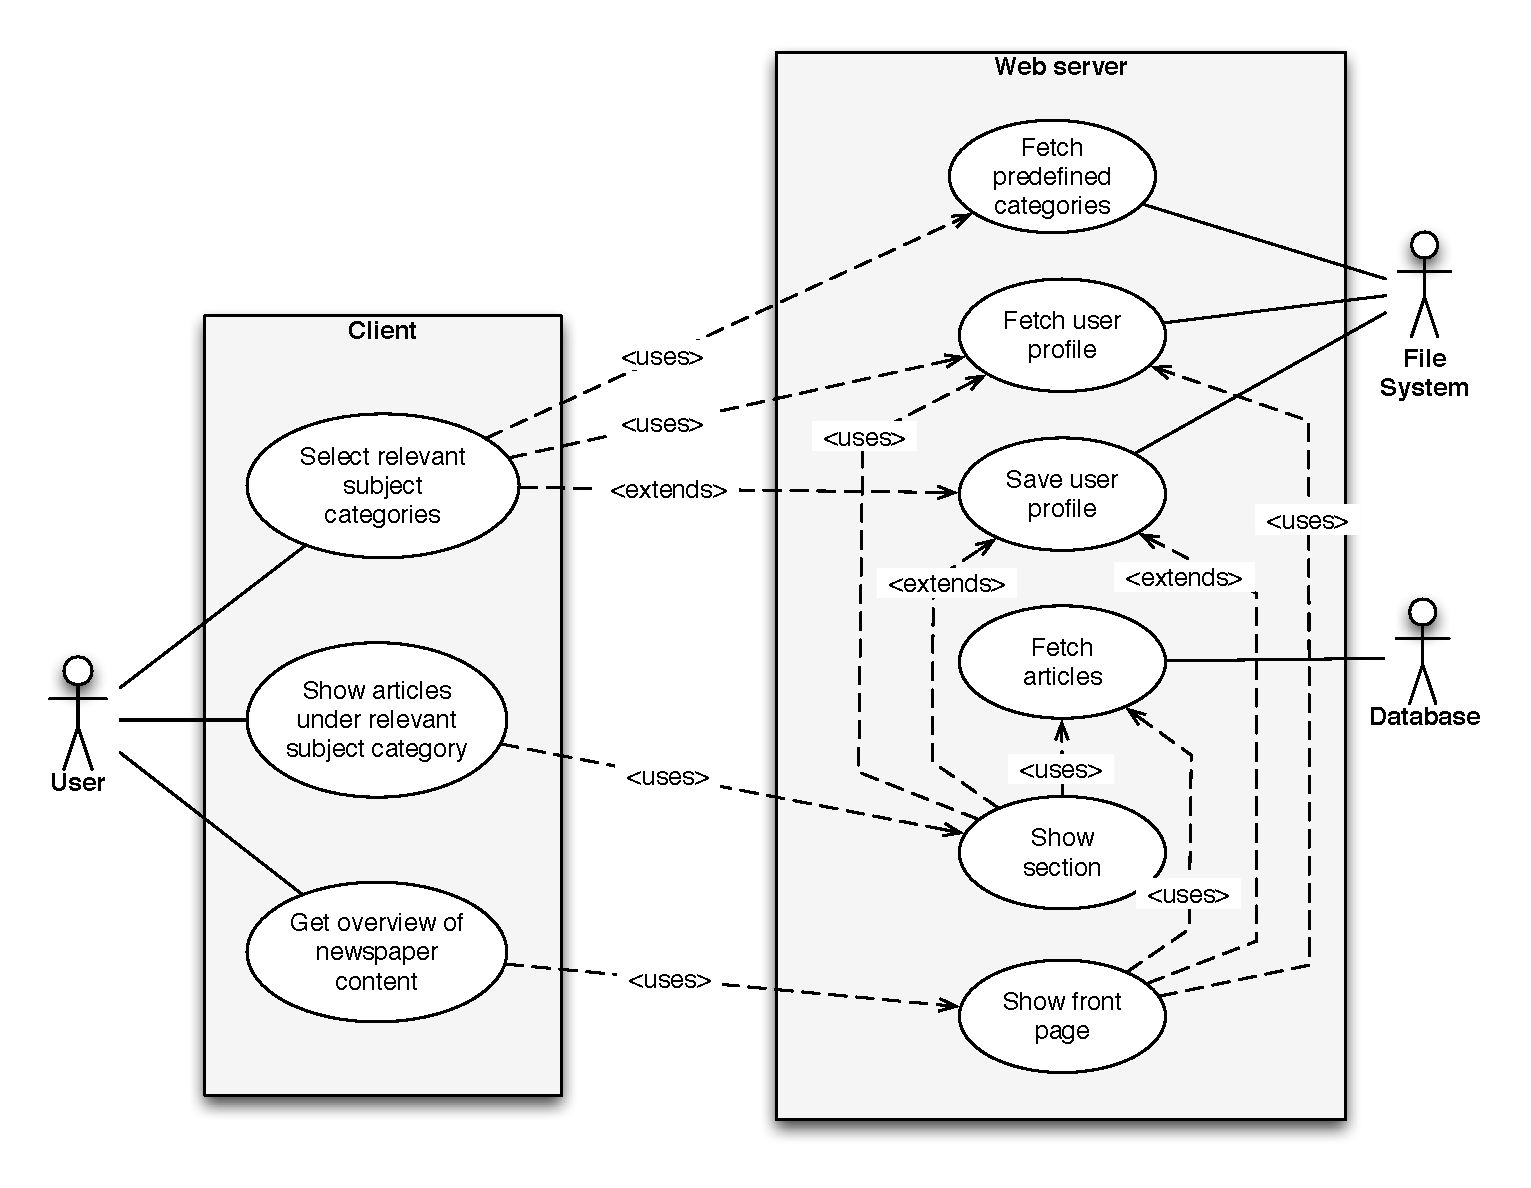
\includegraphics[width=\textwidth]{img/use-cases}}
%	%\newlength{\graphicheight}
%	\settoheight\graphicheight{\mygraphic}
%	\mygraphic
%	\marginnote{
%	\begin{minipage}{\marginparwidth}
%		\vspace{-\graphicheight}%
%		\caption{The figure shows the overall use cases of the system and how the web server acts to accomplish them.}
%		\label{fig:use-cases}
%		\vspace{\graphicheight}
%		\end{minipage}
%	}
%\end{figure}

%\usepackage[wide,outercaption]{sidecap}
%\usepackage[style=philosophy-modern,hyperref,square,natbib]{biblatex}
%------------------------------------------------			

%\PassOptionsToPackage{square,numbers}{natbib}
% \usepackage{natbib}

\usepackage{chngpage}
\usepackage{calc}
\usepackage{listings}
\usepackage{graphicx}
\usepackage[lofdepth,lotdepth]{subfig}

\newlength\largefigure % to create a new length
\setlength{\largefigure}{\columnwidth+\marginparsep+%
\marginparwidth}

%\usepackage{subfigure}
%\newcommand{\goodgap} {\hspace{\subfigtopskip} \hspace{\subfigbottomskip}}
\setkeys{Gin}{width=\linewidth,totalheight=\textheight,keepaspectratio}
%\usepackage{subfig}
\usepackage{multicol}
\usepackage{makeidx}
\usepackage{fixltx2e}
\usepackage{relsize}
\usepackage{lipsum} 
\usepackage[eulerchapternumbers,listings,drafting,pdfspacing,subfig,beramono,parts]{classicthesis} %floatperchapter,%linedheaders,%%eulermath,
%\usepackage{arsclassica}

\usepackage{todonotes}

\usepackage{clrscode3e}
%\newcommand\todonote[1]{\textcolor{red}{\todo[bordercolor=red,backgroundcolor=white,inline]{? #1}}}

\newcommand\itemdist{\setlength{\itemsep}{6pt}
  \setlength{\parskip}{0pt}
  \setlength{\parsep}{0pt}}

% ****************************************************************************************************
% 1. Configure classicthesis for your needs here, e.g., remove "drafting" below 
% in order to deactivate the time-stamp on the pages
% ****************************************************************************************************
\PassOptionsToPackage{eulerchapternumbers,listings,drafting,%
                 pdfspacing,%floatperchapter,%linedheaders,%
                 subfig,beramono,parts}{classicthesis}    

\usepackage{xspace} % To get the spacing after macros right

\addtolength{\parskip}{\baselineskip}
 \setlength{\parindent}{0pt}

\newcommand{\myTitle}{Personalising the Editorial Mix for a Digital Newspaper using Constraint Programming\xspace}
%\newcommand{\mySubtitle}{An Homage to The Elements of Typographic Style\xspace}
%\newcommand{\myDegree}{Doktor-Ingenieur (Dr.-Ing.)\xspace}
\newcommand{\myName}{Michael Lun\o e\xspace}
%\newcommand{\myProf}{Put name here\xspace}
%\newcommand{\myOtherProf}{Put name here\xspace}
\newcommand{\mySupervisor}{Michael Kai Petersen\xspace}
\newcommand{\myOtherSupervisor}{Carsten Witt\xspace}
%\newcommand{\myFaculty}{\xspace}
\newcommand{\myDepartment}{Department of Informatics and Mathematical Modelling\xspace}
\newcommand{\myUni}{Technical University of Denmark\xspace}
\newcommand{\myLocation}{Kgs. Lyngby\xspace}
\newcommand{\myTime}{August 2012\xspace}
%\newcommand{\myVersion}{}


%----------------------------------------------------------------------------------------
%   HYPERREFERENCES
%----------------------------------------------------------------------------------------

\PassOptionsToPackage{hyperfootnotes=false,pdfpagelabels}{hyperref}%,pdftex,
\usepackage{hyperref}  % backref linktocpage pagebackref
\pdfcompresslevel=9
\pdfadjustspacing=1
\sloppy

\hypersetup{
% Uncomment the line below to remove all links (to references, figures, tables, etc)
%draft, 
colorlinks=true, linktocpage=true, pdfstartpage=3, pdfstartview=FitV,
% Uncomment the line below if you want to have black links (e.g. for printing black and white)
%colorlinks=false, linktocpage=false, pdfborder={0 0 0}, pdfstartpage=3, pdfstartview=FitV, 
breaklinks=true, pdfpagemode=UseNone, pageanchor=true, pdfpagemode=UseOutlines,
plainpages=false, bookmarksnumbered, bookmarksopen=true, bookmarksopenlevel=1,
hypertexnames=true, pdfhighlight=/O, urlcolor=webbrown, linkcolor=RoyalBlue, citecolor=webgreen,
%------------------------------------------------
% PDF file meta-information
pdftitle={\myTitle},
pdfauthor={\textcopyright\ \myName, \myUni, \myDepartment},
pdfsubject={},
pdfkeywords={},
pdfcreator={pdfLaTeX},
pdfproducer={LaTeX with hyperref and classicthesis}
%------------------------------------------------
}
% ********************************************************************
% hyperref
% ******************************************************************** 
\newcommand{\mail}[1]{\href{mailto:#1}{\texttt{#1}}}

%----------------------------------------------------------------------------------------
%   BACKREFERENCES
%----------------------------------------------------------------------------------------
\usepackage{ifthen} % Allows the user of the \ifthenelse command
\newboolean{enable-backrefs} % Variable to enable backrefs in the bibliography
\setboolean{enable-backrefs}{false} % Variable value: true or false

\newcommand{\backrefnotcitedstring}{\relax} % (Not cited.)
\newcommand{\backrefcitedsinglestring}[1]{(Cited on page~#1.)}
\newcommand{\backrefcitedmultistring}[1]{(Cited on pages~#1.)}
\ifthenelse{\boolean{enable-backrefs}} % If backrefs were enabled
{
\PassOptionsToPackage{hyperpageref}{backref}
\usepackage{backref} % to be loaded after hyperref package 
\renewcommand{\backreftwosep}{ and~} % separate 2 pages
\renewcommand{\backreflastsep}{, and~} % separate last of longer list
\renewcommand*{\backref}[1]{}  % disable standard
\renewcommand*{\backrefalt}[4]{% detailed backref
\ifcase #1 
\backrefnotcitedstring
\or
\backrefcitedsinglestring{#2}
\else
\backrefcitedmultistring{#2}
\fi}
}{\relax} 

%----------------------------------------------------------------------------------------
%   AUTOREFERENCES SETUP
%   Redefines how references in text are prefaced for different 
%   languages (e.g. "Section 1.2" or "section 1.2")
%----------------------------------------------------------------------------------------

\makeatletter
\@ifpackageloaded{babel}
{
\addto\extrasbritish{
\renewcommand*{\figureautorefname}{Figure}
\renewcommand*{\tableautorefname}{Table}
\renewcommand*{\partautorefname}{Part}
\renewcommand*{\chapterautorefname}{Chapter}
\renewcommand*{\sectionautorefname}{Section}
\renewcommand*{\subsectionautorefname}{Section}
\renewcommand*{\subsubsectionautorefname}{Section}
}
\providecommand{\subfigureautorefname}{\figureautorefname} % Fix to getting autorefs for subfigures right
}{\relax}
\makeatother


% ********************************************************************
% makeidx, multicol
% ********************************************************************
\let\orgtheindex\theindex
\let\orgendtheindex\endtheindex
\def\theindex{%
	\def\twocolumn{\begin{multicols}{2}}%
	\def\onecolumn{}%
	\clearpage
	\orgtheindex
}
\def\endtheindex{%
	\end{multicols}%
	\orgendtheindex
}

\makeindex


% ********************************************************************
% listings
% ********************************************************************


\definecolor{lightergray}{gray}{0.99}

\lstset{language=[LaTeX]Tex,
    keywordstyle=\color{RoyalBlue},
    basicstyle=\normalfont\ttfamily,
    commentstyle=\color{Emerald}\ttfamily,
    stringstyle=\rmfamily,
    numbers=none,
    numberstyle=\scriptsize,
    stepnumber=5,
    numbersep=8pt,
    showstringspaces=false,
    breaklines=true,
    frameround=ftff,
    frame=lines,
    backgroundcolor=\color{lightergray}
} 

\lstset{	morekeywords=%
        {RequirePackage,newboolean,DeclareOption,setboolean,%
        ProcessOptions,PackageError,ifthenelse,boolean,%
        chapterNumber,sodef,textls,allcapsspacing,%
        MakeTextLowercase,orgtheindex,endtheindex,%
        @ifpackageloaded,undefined,sfdefault,%
        DeclareRobustCommand,spacedallcaps,%
        microtypesetup,MakeTextUppercase,lowsmallcapsspacing,%
        lowsmallcapsspacing,spacedlowsmallcaps,
        spacedlowsmallcaps,lehead,headmark,color,%
        headfont,partname,thepart,titleformat,part,
        titlerule,chapter,thechapter,thesection,%
        subsection,thesubsection,thesubsubsection,%
        paragraph,theparagraph,descriptionlabel,titlespacing,%
        graffito,lineskiplimit,finalhyphendemerits,%
        colorbox,captionsetup,labelitemi,%
        myincludegraphics,hypersetup,setlength,%
        definecolor,lsstyle,textssc,subsubsection,%
        graffito@setup,includegraphics,ifdefined,%
        myTitle,textcopyright,myName,lstset,lstnewenvironment,%
        setkeys,lst@BeginAlsoWriteFile,contentsname,%
        toc@heading,@ppljLaTeX,z@,check@mathfonts,%
        sf@size,ptctitle,mtctitle,stctitle,lst@intname,%
        @empty,math@fontsfalse,@ppljscTeX,@iwonaTeX,%
        @iwonascLaTeX,@ctTeX,tw@,ct@sc,@ctTeX,f@family,%
        f@shape,ct@sc,ctLaTeX,ctLaTeXe,@twoe,@sctwoe,%
        texorpdfstring,m@th,ctTeX,@mkboth,ProvidesPackage,%
        theindex,PackageInfo,PackageWarningNoLine,%
        mtifont,mtcindent,@iwonaLaTeX,@ppljTeX,@iwonascTeX,%
        rohead,orgendtheindex,@ppljscLaTeX,%
        @ifclassloaded,toc@headingbkORrp,backreftwosep,%
        backrefalt,backreflastsep,areaset,pnumfont,%
        arsincludegraphics,ExecuteOptions,PackageWarning,textcolor,%
        MessageBreak,ars@@includegraphics,ifcld@backref,rofoot,formatchapter,%
        if@twoside},
        commentstyle=\color{Emerald}\ttfamily,%
        frame=lines}

\lstset{basicstyle=\normalfont\ttfamily}
\lstset{flexiblecolumns=true}
\lstset{moredelim={[is][\normalfont\itshape]{/*}{*/}}}
\lstset{basicstyle=\normalfont\ttfamily}
\lstset{flexiblecolumns=false}
\lstset{moredelim={[is][\ttfamily]{!?}{?!}}} 
\lstset{escapeinside={�*}{*�}}
\lstset{firstnumber=last}
\lstset{moredelim={[is][\ttfamily]{!?}{?!}}}

\DeclareRobustCommand*{\pacchetto}[1]{{\normalfont\ttfamily#1}%
\index{Pacchetto!#1@\texttt{#1}}%
\index{#1@\texttt{#1}}}

\DeclareRobustCommand*{\bibtex}{\textsc{Bib}\TeX%
\index{bibtex@\textsc{Bib}\protect\TeX}%
}

%\DeclareRobustCommand*{\amseuler}{\protect\AmS{} Euler%
%\index{AmS Euler@\protect\AmS~Euler}%
%\index{Font!AmS Euler@\protect\AmS~Euler}}

\lstnewenvironment{code}% 
{\setkeys{lst}{columns=fullflexible,keepspaces=true}%
\lstset{basicstyle=\small\ttfamily}%
}{}

\lstset{extendedchars} 
\lstnewenvironment{sidebyside}{% 
    \global\let\lst@intname\@empty 
    \setbox\z@=\hbox\bgroup 
    \setkeys{lst}{columns=fullflexible,% 
    linewidth=0.45\linewidth,keepspaces=true,%
    breaklines=true,% 
    breakindent=0pt,%
    boxpos=t,%
    basicstyle=\small\ttfamily
}% 
    \lst@BeginAlsoWriteFile{\jobname.tmp}% 
}{% 
    \lst@EndWriteFile\egroup 
        \begin{center}% 
            \begin{minipage}{0.45\linewidth}% 
                \hbox to\linewidth{\box\z@\hss} 
            \end{minipage}% 
            \qquad 
            \begin{minipage}{0.45\linewidth}%
            \setkeys{lst}{frame=none}% 
                \leavevmode \catcode`\^^M=5\relax 
                \small\input{\jobname.tmp}% 
            \end{minipage}% 
        \end{center}% 
} 

\newcommand{\omissis}{[\dots\negthinspace]}

%\graphicspath{{img}}

%\hyphenation{Robert Bring-hurst DejaVu
%Bera Mono Vera Classic-Thesis suite Knuth Zapf}

\newcommand{\meta}[1]{$\langle${\normalfont\itshape#1}$\rangle$}
\lstset{escapeinside={�*}{*�}}


\DeclareRobustCommand*{\miktex}{MiK\TeX%
\index{miktex@MiK\protect\TeX}%
}

\DeclareRobustCommand*{\metafont}{\MF%
\index{METAFONT@\protect\MF}%
}

\DeclareRobustCommand*{\metapost}{\MP%
\index{METAPOST@\protect\MP}%
}

\DeclareRobustCommand*{\texlive}{\TeX{}~Live%
\index{texlive@\protect\TeX{}~Live}%
}

%----------------------------------------------------------------------------------------
%   USEFUL COMMANDS
%----------------------------------------------------------------------------------------

\newcommand{\ie}{i.\,e.}
\newcommand{\Ie}{I.\,e.}
\newcommand{\eg}{e.\,g.}
\newcommand{\Eg}{E.\,g.} 

\usepackage{todonotes}
%\newcommand\todonote[1]{\textcolor{red}{\todo[bordercolor=red,backgroundcolor=white,inline]{? #1}}}

\newcounter{dummy} % Necessary for correct hyperlinks (to index, bib, etc.)
\providecommand{\mLyX}{L\kern-.1667em\lower.25em\hbox{Y}\kern-.125emX\@}


\PassOptionsToPackage{smaller}{acronym} % Include printonlyused in the first bracket to only show acronyms used in the text
\usepackage{acronym} % nice macros for handling all acronyms in the thesis

%------------------------------------------------

%\renewcommand*{\acsfont}[1]{\textssc{#1}} % For MinionPro
\renewcommand{\bflabel}[1]{{#1}\hfill}

%------------------------------------------------

\PassOptionsToPackage{pdftex}{graphicx}
\usepackage{graphicx}
\usepackage[lofdepth,lotdepth]{subfig}
%\usepackage{subfigure}
%\newcommand{\goodgap} {\hspace{\subfigtopskip} \hspace{\subfigbottomskip}}
\setkeys{Gin}{width=\linewidth,totalheight=\textheight,keepaspectratio}


%----------------------------------------------------------------------------------------
%   FLOATS: TABLES, FIGURES AND CAPTIONS SETUP
%----------------------------------------------------------------------------------------

\usepackage{tabularx} % Better tables
\setlength{\extrarowheight}{3pt} % Increase table row height
\newcommand{\tableheadline}[1]{\multicolumn{1}{c}{\spacedlowsmallcaps{#1}}}
\newcommand{\myfloatalign}{\centering} % To be used with each float for alignment
%\usepackage{caption}
%\captionsetup{format=hang,font=small}
%\usepackage{subfig} 


% ********************************************************************
% biblatex
% ******************************************************************** 

%\bibliography{Bibliography}
%
%\renewcommand{\nameyeardelim}{, }
%
%\defbibheading{bibliography}{%
%\cleardoublepage
%\manualmark
%\phantomsection
%\addcontentsline{toc}{chapter}{\tocEntry{\bibname}}
%\chapter*{\bibname\markboth{\spacedlowsmallcaps{\bibname}}
%{\spacedlowsmallcaps{\bibname}}}}     
%
%  \DeclareCiteCommand{\citeyearpar}[\mkbibparens] 
%  {\boolfalse{citetracker}% 
%   \boolfalse{pagetracker}% 
%   \usebibmacro{prenote}} 
%  {\printtext[bibhyperref]{\printfield{year}}} 
%  {\multicitedelim} 
%  {\usebibmacro{postnote}} 
%
%\makeatletter 
%  \DeclareCiteCommand{\citetalias} 
%  {\usebibmacro{prenote}} 
%  {\usebibmacro{citeindex}% 
%   \bibhyperref{\@citealias{\thefield{entrykey}}}} 
%  {\multicitedelim} 
%  {\usebibmacro{postnote}} 
%\makeatother 

%\setcounter{biburlnumpenalty}{9000}
%\setcounter{biburlucpenalty}{9000}
%\setcounter{biburllcpenalty}{9000}


% ********************************************************************
% other commands
% ******************************************************************** 

%\newcommand{\ita}[1]{% 
%  \begin{otherlanguage*}{italian}#1\end{otherlanguage*}}
  
%\DeclareRobustCommand*{\pkgname}[1]{{\normalfont\sffamily#1}%
%\index{Package!#1@\textsf{#1}}%
%\index{#1@\textsf{#1}}}
%
%\DeclareRobustCommand*{\envname}[1]{{\normalfont\ttfamily#1}%
%\index{Environment!#1@\texttt{#1}}%
%\index{#1@\texttt{#1}}}
%
%\DeclareRobustCommand*{\optname}[1]{{\normalfont\ttfamily#1}%
%\index{Option!#1@\texttt{#1}}%
%\index{#1@\texttt{#1}}}
%
%\DeclareRobustCommand*{\clsname}[1]{{\normalfont\sffamily#1}%
%\index{Class!#1@\textsf{#1}}%
%\index{#1@\textsf{#1}}}
%
%\DeclareRobustCommand*{\cmdname}[1]{\mbox{\lstinline!\\#1!}%
%\index{#1@\texttt{\hspace*{-1.2ex}\textbackslash#1}}}
%
%\DeclareRobustCommand*{\classicthesis}{Classic\-Thesis}
%
%\DeclareRobustCommand*{\arsclassica}{{\normalfont\sffamily ArsClassica}}
%
%\DeclareRobustCommand*{\miktex}{MiK\TeX%
%\index{miktex@MiK\protect\TeX}}
%
%\DeclareRobustCommand*{\texlive}{\TeX{}~Live%
%\index{texlive@\protect\TeX{}~Live}}




%\renewcommand{\sfdefault}{amsfonts}
%\usepackage{sfmath}
%\renewcommand{\rmdefault}{amsfonts}
%\usepackage[osf,sc]{mathpazo}
%\renewcommand{\rmdefault}{ppl}
%\renewcommand{\scdefault}{ppl}
%\renewcommand{\sfdefault}{ppl}
%\linespread{1.05}
\renewcommand*\ttdefault{lmtt}

% General Tips:
% 1) Make sure to edit the classicthesis-config.file
% 2) New enumeration (A., B., C., etc in small caps): \begin{aenumerate} \end{aenumerate}
% 3) For margin notes: \marginpar or \graffito{}
% 4) Do not use bold fonts in this style, it is designed around them
% 5) Use tables as in the examples
% 6) See classicthesis-preamble.sty for useful commands

\begin{document}

\frenchspacing % Reduces space after periods to make text more compact

\raggedbottom % Makes all pages the height of the text on that page

\selectlanguage{british} % Select your default language - e.g. american or ngerman

%\renewcommand*{\bibname}{new name} % Uncomment to change the name of the bibliography
%\setbibpreamble{} % Uncomment to include a preamble to the bibliography - some text before the reference list starts

\pagenumbering{roman} % Roman page numbering prior to the start of the thesis content (i, ii, iii, etc)

\pagestyle{plain} % Suppress headers for the pre-content pages

%----------------------------------------------------------------------------------------
%	PRE-CONTENT THESIS PAGES
%----------------------------------------------------------------------------------------

\include{FrontBackmatter/Titlepage} % Main title page

\include{FrontBackmatter/Titleback} % Back of the title page

%\cleardoublepage\include{FrontBackmatter/Dedication} % Dedication page

%\cleardoublepage\include{FrontBackmatter/Foreword} % Uncomment and create a Foreword.tex to include a foreword

\cleardoublepage%!TEX root = ../thesis.tex
% Abstract
\pdfbookmark{Abstract}{Abstract}
\begingroup
\let\clearpage\relax
\let\cleardoublepage\relax
\let\cleardoublepage\relax

\chapter*{Abstract}
This paper proposes a Constraint Programming (CP) approach to personalise a composition of articles that follows rules of the editorial mix in a digital newspaper. Inspiration from conventional newspapers will be used to express the problem as a Constraint Optimisation Problem and solved using local search for CP taking advantage of both probabilistic and logical approaches. Furthermore, this paper proposes a keyword based solution, using WordNet enrichment of articles in combination with a comparison of entities, to determine the relevance of an article to a user defined topic and similarity between articles. As a by-product of the implementation a library for solving personalisation problems using CP was developed.

\vfill

%\selectlanguage{danish}
\pdfbookmark[1]{Resumé}{Resumé}
\chapter*{Resumé}
Denne afhandling præsenterer Constraint Programming (CP) anvendt til at personalisere sammensætningen af artikler i en digital avis, der følger redaktionelle regler. Med inspiration hentet fra konventionelle aviser bliver de redaktionelle regler udtrykt som et Constraint Optimisation Problem og løst vha. local search teknikker for CP. Dette gør at både probalistiske og logiske fordele bliver udnyttet. Udover dette bliver en keywordbaseret løsning præsenteret til at udregne relevans af de enkelte artikler ift. brugerdefinerede emner, men også artiklerne imellem. Løsningen gør brug af WordNet til at berige artiklerne og en sammenligning af entiteter til den semantiske analyse. Som et bi-produkt af implementeringen blev der udviklet et bibliotek til at løse personaliseringsproblemer vha. CP.

%\selectlanguage{british}

\endgroup			

\vfill

%\pdfbookmark[1]{Abstract}{Abstract} % Bookmark name visible in a PDF viewer
%
%\begingroup
%\let\clearpage\relax
%\let\cleardoublepage\relax
%\let\cleardoublepage\relax
%
%\chapter*{Abstract} % Abstract name
%
%Short summary of the contents\dots
%%\todo[inline]{Til Chris: Tusind tak for hjælpen! :)}
%
%\endgroup			

\vfill % Abstract page
\cleardoublepage%*******************************************************
% Acknowledgements
%*******************************************************
\pdfbookmark{Acknowledgements}{Acknowledgements}

\begingroup
\let\clearpage\relax
\let\cleardoublepage\relax
\let\cleardoublepage\relax

\chapter*{Acknowledgements}

I wish first of all to thank my family and friends for great support and for review of the paper. Without their support I would not have come as far as I hoped. I would also like to thank my counsellors, Michael Kai Petersen and Carsten Witt from the Department of Informatics and Mathematical Modelling at the Technical University of Denmark, for giving me room for my own definition of the project. They have both been a great aid in the process with guidance and review of the paper.

%Finally, a special thanks to Jens for odd discussions and help in the process, Bo and Niklas for assistance with their knowledge, Ditte for the help and review and my brother and father for all the support.
Finally, a special thanks to Jens for odd discussions and help in the process, Bo and Niklas for assistance with their knowledge and my brother and father for all the support.

\endgroup




%\cleardoublepage\include{FrontBackmatter/01_abstract} % Abstract page
%\cleardoublepage%!TEX root = thesis.tex
%\chapter{} %{Sammenfatning (Summary in Danish)}

\pdfbookmark[1]{Resum\'e}{Resum\'e} % Bookmark name visible in a PDF viewer

\begingroup
\let\clearpage\relax
\let\cleardoublepage\relax
\let\cleardoublepage\relax

\chapter*{Resum\'e} % Abstract name

Kort resum\'e af indholdet\dots
%Projektet præsenterer den grundlæggende teori bag Constraint Programming (CP) og playlists. Strategien i arbejdet med constraints, logisk og funktionel programmering er anvendt til at opstille en Automatic Playlist Generator, som også benytter sig af en funktion til at sammenligne musiknumre. Produktet af projektet er et program i SML der genererer playlists ud fra forslag og forbud på sange fra et bibliotek. Funktionen til sammenligning er alene baseret på sammenligning imellem tempo og toner (key), som resulterer i forholdsvist ubruglige playlists. Programmet mangler sammenligninger imellem klangfarve (timbre), rytme og melodi, men den dynamiske tilgang gør at det let kan implementeres. Til sidst sluttes af den anvendte CP og local search tilgang viser sig effektiv til at løse problemet.

\endgroup			

\vfill % Abstract page
\cleardoublepage%!TEX root = thesis.tex
\chapter{Preface}
%Time spent on assembling playlists for certain purposes often exceeds the actual use. Some automatic playlist generation engines already exists, but they often lack the possibility of altering the generated playlist - or the option of specifying the length. The result is a repeated query for a playlist until one satisfies and another when it runs out of songs to play.
%
%This thesis is the product of a personal need for an Automatic Playlist Generator.
%
%The thesis is produced under the Department of Informatics and Mathematical Modelling at the Technical University of Denmark and it will presume some knowledge of logic programming and functional programming as it will include an implementation of a program in each language. The preconditions for the thesis are the courses 02156 Formal Logical Systems and 02157 Functional programming taught at the Technical University of Denmark.

\vspace{20mm}
\mbox{}\hfill
\begin{minipage}[t]{80mm}
  Kgs. Lyngby, June 2012
  \\ \\
  \mbox{} \hspace{-16mm} \includegraphics{img/signature.eps}
  Michael Lunøe
\end{minipage}
 % Abstract page
%\cleardoublepage%!TEX root = thesis.tex
\chapter{Acknowledgements}

I would like to thank my family and friends for support and review of the thesis. I would also like to thank my counsellors, Michael Kai Petersen and Carsten Witt from the Department of Informatics and Mathematical Modelling at the Technical University of Denmark, for giving me room for my own definition of the thesis. Also for review of the process and guidance in the right direction.
 % Acknowledgements page

%\cleardoublepage\include{FrontBackmatter/Publication} % Publications from the thesis page

\pagestyle{scrheadings} % Show chapter titles as headings

\cleardoublepage%!TEX root = ../thesis.tex
% Table of Contents - List of Tables/Figures/Listings and Acronyms

\refstepcounter{dummy}

\pdfbookmark[1]{\contentsname}{tableofcontents} % Bookmark name visible in a PDF viewer

\setcounter{tocdepth}{1} % Depth of sections to include in the table of contents - currently up to subsections

\setcounter{secnumdepth}{3} % Depth of sections to number in the text itself - currently up to subsubsections

\manualmark
\markboth{\spacedlowsmallcaps{\contentsname}}{\spacedlowsmallcaps{\contentsname}}
\tableofcontents 
\automark[section]{chapter}
\renewcommand{\chaptermark}[1]{\markboth{\spacedlowsmallcaps{#1}}{\spacedlowsmallcaps{#1}}}
\renewcommand{\sectionmark}[1]{\markright{\thesection\enspace\spacedlowsmallcaps{#1}}}

\clearpage

\begingroup 
\let\clearpage\relax
\let\cleardoublepage\relax
\let\cleardoublepage\relax

%----------------------------------------------------------------------------------------
%	List of Figures
%----------------------------------------------------------------------------------------
%
%\refstepcounter{dummy}
%%\addcontentsline{toc}{chapter}{\listfigurename} % Uncomment if you would like the list of figures to appear in the table of contents
%\pdfbookmark[1]{\listfigurename}{lof} % Bookmark name visible in a PDF viewer
%
%\listoffigures
%
%\vspace*{8ex}
%\newpage
%
%%----------------------------------------------------------------------------------------
%%	List of Tables
%%----------------------------------------------------------------------------------------
%
%\refstepcounter{dummy}
%%\addcontentsline{toc}{chapter}{\listtablename} % Uncomment if you would like the list of tables to appear in the table of contents
%\pdfbookmark[1]{\listtablename}{lot} % Bookmark name visible in a PDF viewer
%
%\listoftables
%        
%\vspace*{8ex}
%\newpage
%    
%%----------------------------------------------------------------------------------------
%%	List of Listings
%%---------------------------------------------------------------------------------------- 
%
%\refstepcounter{dummy}
%%\addcontentsline{toc}{chapter}{\lstlistlistingname} % Uncomment if you would like the list of listings to appear in the table of contents
%\pdfbookmark[1]{\lstlistlistingname}{lol} % Bookmark name visible in a PDF viewer
%
%\lstlistoflistings 
%
%\vspace*{8ex}
%\newpage
       
%----------------------------------------------------------------------------------------
%	Acronyms
%----------------------------------------------------------------------------------------

\refstepcounter{dummy}
%\addcontentsline{toc}{chapter}{Acronyms} % Uncomment if you would like the acronyms to appear in the table of contents
\pdfbookmark[1]{Acronyms}{acronyms} % Bookmark name visible in a PDF viewer

\markboth{\spacedlowsmallcaps{Acronyms}}{\spacedlowsmallcaps{Acronyms}}

\chapter*{Acronyms}

\begin{acronym}[]
\acro{API}{Application Programming Interface: A specification intended to be used as an interface by software components to communicate with each other.}
\acro{CP}{Constraint Programming: Constraint programming is a programming paradigm wherein relations between variables are stated in the form of constraints.}
\acro{CSP}{Constraint Satisfaction Problem: Mathematical problems defined as a set of objects whose state must satisfy a number of constraints or limitations.}
\acro{COP}{Constraint Optimisation Problem: Can be defined as a regular constraint satisfaction problem in which constraints are weighted and the goal is to find a solution maximizing the weight of satisfied constraints.}
\acro{RSS}{Really Simple Syndication: A family of web feed formats used to publish frequently updated works—such as blog entries, news headlines, audio, and video—in a standardized format.}
% .*, Aa: [A-Z][A-Z]+
% .*: \\emph\{(\w)*
\end{acronym}  
                   
\endgroup

\cleardoublepage % Contents, list of figures/tables/listings and acronyms

\pagenumbering{arabic} % Arabic page numbering for thesis content (1, 2, 3, etc)
%\setcounter{page}{90} % Uncomment to manually start the page counter at an arbitrary value (for example if you wish to count the pre-content pages in the page count)

\cleardoublepage % Avoids problems with pdfbookmark

%----------------------------------------------------------------------------------------
%	THESIS CONTENT - CHAPTERS
%----------------------------------------------------------------------------------------


\ctparttext{Discussing solutions to the problem of automatically generating the editorial mix and identifying rules that constitute the editorial mix.} % Text on the Part 1 page describing  the content in Part 1
\part{Defining the problem} % First part of the thesis

%\include{Chapter01} % Chapter 1

%!TEX root = ../thesis.tex
\chapter{Creating the Editorial Mix} % (fold)
\label{ch:introduction}
This chapter introduces the editorial mix of a digital newspaper and which parameters to account for when composing the newspaper. It is afterwards discussed which of these parameters are suited for personalisation, and how this can be done. The proposed approach is then presented with its pros and cons, which results in a list of contributions this project has to the field of personalisation.
%\todo[inline]{Introduce an automated editorial mix to the digital newspaper. Bringing rss-readers and digital newspapers closer together.}

\section{What is the Editorial Mix}
In the conventional newspapers the editors job is to compose an intriguing front page that offers the contents of the sections that might interest the individual user. His challenge is to accommodate the needs of the newspapers segment of readers, divide the articles into sections, with a nice reading flow and attractive illustrations, and hand-pick articles to go on the front page. But what if a computer could do this?
%"their segment of readers", hvis readers? Måske det ville lyde bedre hvis man skrev "the paper's segment of readers" eller noget i den dur.

\cite{perkowitz-Adaptive-Web-Sites} decomposes the problem of synthesising adapted page into several subproblems\sidenote{In the subproblems stated here, ``hyperlink'' has been replaced by ``item'' to appreciate them more generally, rather than the original specific sense.}:
\begin{itemize}
	\item What is the content (that is, set of items) of the index page?
	\item Does it have a coherent topic? What should its title be?
	\item How are the items on the page ordered?
	\item How are the items labeled?
	\item Is the page consistent with the site's overall graphical style?
	\item Is it appropriate to add the page to the site? If so, where?
\end{itemize}

Some efforts have been made to digitally calculate similarities between articles and based on a current article suggest similar reading material or use collaborate filtering to suggest articles based on other users reading behaviour. Some papers proposes a composition of articles from user picked RSS-feeds, which can, e.g.\ in the case of Google Reader, be divided into sections. This comes close to conventional newspapers, but there is no ordering of the flow of articles. The ordering, flow and choice of relevant articles is here on referred to as the \emph{relational} part of the editorial mix.
% "Others offer composition of articles..." Others giver ikke mening her, hvem mener du?

The solution for some digital newspapers are still to have an editor to create their coherent composed digital newspaper, like the New York Times or Wired Magazine. Flipboard, on the other hand, composes their editorial mix of articles from feeds and divides their pages  into three or more rarely four or five articles\sidenote{Flipboard includes specialised layouts with more articles per page for Twitter.} with excerpts and images, much like conventional newspapers front pages. How they choose their composition is kept a business secret, but it does seem to vary a lot, see Figure~\ref{fig:flipboard-screenshot}.

\begin{figure}[h!tb]
 	\begin{center}
 		\includegraphics[width=.45\textwidth]{img/flipboard2}
 	\end{center}
 	\caption{A screenshot of composition of three articles in Flipboard, with different subjects, i.e.\ world crime, world finance and technology news.}
 	\label{fig:flipboard-screenshot}
\end{figure}

\todo[inline]{Maybe put in a reference to a conventional newspaper.}

It is hard to say if there is a control behind the placement of content other than the choice of featured and non-featured articles, but this is actually an example of a computationally composed newspaper. The placement and amount of room given for an article is here on referred to as the \emph{spacial} part of the editorial mix.

Finally, subjects of articles have more relevance at some points in time than others and editors choose the amount of time stories should be available in, where RSS-readers just displays the newest articles first, which are not always the most relevant. This selection of articles within a chosen time frame is here on referred to as the \emph{temporal} part of the editorial mix.

One thing that is vastly different from newspapers to RSS-readers is the ability to deliver personalised content, in that a user can choose which RSS-feeds to follow, whereas readers of newspapers need to navigate it in order to find interesting articles. Also where newspapers have quality assurance of its content, RSS-readers have a seemingly unlimited amount of articles.

\section{Personalising a Digital Newspaper}
\cite{BushMemex} describes a collective memory library machine that can be indexed, called the memex. Items in the library are linked together forming personal association trails. This is the early conception of the hypertext media that would later become the World Wide Web and later personalised web applications. With many respects that is what this project tries to achieve; i.e.\ link information in the form of articles together and present them in personalised trials defined by the user. As opposed to \cite{BushMemex} proposed manual linking it is now possible to, e.g.\ classify and compute similarity automatically, which greatly aids the process. 

User preferences are very diverse and it is therefore hard to accommodate every individual in a single solution. A digital solution must be bound to a specific domain, but must also be open for novel use.

%\begin{quotation}
%	``Web personalization is the process of customizing a Web site to the needs of specific users, taking advantage of the knowledge acquired from the analysis of the user's navigational behavior (usage data) in correlation with other information collected in the Web context, namely, structure, content, and user profile data.'' \cite{MagdaliniWebMining}
%\end{quotation}
\begin{minipage}{.8\largefigure}
\begin{flushleft}{\slshape
``Web personalization is defined as any action that adapts the information or services provided by a Web site to the needs of a particular user or a set of users, taking advantage of the knowledge gained from the users' navigational behavior and individual interests, in combination with the content and the structure of the Web site.''} \\ \medskip
-- \cite{MagdaliniWebMining}
\end{flushleft}
\end{minipage}
	
%\cite{WebMiningMulvenna} defines the goal of personalisation systems as follows: ``to provide users with the information they want or need, without expecting from them to ask for it explicitly''

The three categories of the editorial mix can be described in the sense of personalisation as well. Accommodating user preference based on spacial personalisation is achieved by a placement of articles, temporal personalisation by selecting articles of higher news value based on their relevance time frame and finally, relational personalisation by selecting articles that provides more value based on their respective and collaborate topics. Temporal personalisation is also obtained by letting user preferences have a life time and decrease the preference influence on which articles to select as time passes.
%Der er noget galt her, men er ikke helt sikker på hvad: "decrease its in influence.."

All three categories are related as they each provide some value to the editorial mix, e.g.\ a different spacial placement of a specific article can provide a different composition of the editorial mix and therefore a different temporal and/or relational value to the user.
%or the editorial composition/arrangement

\section{Contributions of Constraint Programming}
\hspace{-\marginparwidth}
\begin{minipage}{.8\largefigure}
\begin{flushright}{\slshape
	``Informally, declarative programming involves stating \emph{what} is computed, but not necessarily \emph{how} it is computed. Equivalently, in the terminology of Kowalski's equation $algorithm = logic + control$, it involves stating the \emph{logic} of an algorithm, but not necessarily the \emph{control}.''} \\ \medskip
-- \cite{LloydDeclarative}
\end{flushright}
\end{minipage}
%
%\begin{quotation}
%``The logic component determines the meaning of the algorithm whereas the control component only affects its efficiency [...] When logic is separated from control, it is possible to distinguish (in the logic) what the program does from how the program does it (in the control)'' \cite{KowalskiAlgo}
%\end{quotation}

As a declarative programming language, Constraint Programming (CP) offers means for describing the problem to be solved using constraints and a general purpose constraint solver. Once the general purpose solver is set up, the constraints can be defined to model the problem to be solved, but does not necessarily make it easy. However, the problem definition can easily be extended and/or modified afterwards.

\hspace{-\marginparwidth}
\begin{minipage}{.8\largefigure}
\begin{flushright}{\slshape
	``Ordinary people generally aren't interested (and rightly so) in low-level programming details -- they just want to express the problem in some reasonably congenial way and let the system get on with solving the problem. [...] Having to deal only (or mostly) with the logic component simplifies many things for the programmer. First, (the logic component of) a declarative program is generally easier to write and to understand than a corresponding imperative program. Second, a declarative program is also easier to reason about and to transform, as much current research in functional and logic programming shows.''} \\ \medskip
-- \cite{LloydDeclarative}
\end{flushright}
\end{minipage}

Also, with logic comes precise solutions, but this does not come without a cost as stochastic approaches often beat logic by lengths. However, stochastic variables can be introduced to CP.

%\section{Short Introduction to Constraint Programming}
%\label{sec:CP}
To be able to work with personalisation problems as Constraint Satisfaction Problems (CSPs) or Constraint Optimisation Problems (COPs), these need to be defined. The following descriptions of CSPs and COPs have been modified to fit personalisation problems from the original definitions provided by \cite{AIRussell} and~\cite{CPApt}.

A Constraint Satisfaction Problem is defined by the 3-tuple $(\mathcal{X}, \mathcal{D}, \mathcal{C})$, where $\mathcal{X}$ is the set of variables, $\mathcal{D}$ is the corresponding set of domains and $\mathcal{C}$ is the set of constraints on the variables.

Each variable has sub-domains corresponding to the sub-value of each value. And unlike \cite{AIRussell} and~\cite{CPApt} a constraint is here defined as a function of specific variables returning a boolean value. Therefore the tuple of $n$ variables with $m$ sub-variables and $k$ constraints on $r$ and $s$ number of variables, respectively, can be expanded to:

\begin{align*}
\begin{pmatrix}\vspace{3pt}
	\mathcal{X} :
	\begin{Bmatrix}
		x_1 :
		\begin{pmatrix}
			x_1.a_1\\
			\ldots\\
			x_1.a_m\\
		\end{pmatrix}
		, \cdots,
		x_n :
		\begin{pmatrix}
			x_n.a_1\\
			\ldots\\
			x_n.a_m\\
		\end{pmatrix}
	\end{Bmatrix},\\\vspace{1pt}
	\mathcal{D} :
	\begin{Bmatrix}
		d_1 :
		\begin{pmatrix}
			d_1.a_1\\
			\ldots\\
			d_1.a_m\\
		\end{pmatrix}
		, \cdots,
		d_n :
		\begin{pmatrix}
			d_n.a_1\\
			\ldots\\
			d_n.a_m\\
		\end{pmatrix}
	\end{Bmatrix},\\\hspace{3pt}
	\mathcal{C} :
	\begin{Bmatrix}
		c_1 : func(x_i, \cdots,x_{i+r}) \rightarrow \mathbb{B}, \cdots, c_k : func(x_j, \cdots,x_{j+s}) \rightarrow \mathbb{B}
	\end{Bmatrix}\hspace{3pt}
\end{pmatrix}
\end{align*}
Where $\mathbb{B}$ is either \texttt{true} or \texttt{false}.

A CSP is a subset of a Constraint Optimisation Problem (COP) and a COP is defined by the 4-tuple $(\mathcal{X}, \mathcal{D}, \mathcal{C}, \mathcal{O})$, where the three first elements are defined as in a CSP and $\mathcal{O}$ is a set objective (or cost) functions on variables, that determines the quality of a current state. The set of objective functions can be described with the same structure as constraints in CSPs and can be expanded as follows with $l$ number of functions on $t$ and $u$ number of variables, respectively.

\begin{align*}
	\mathcal{O} :
	\begin{Bmatrix}
		o_1 : func(x_i, \cdots,x_{i+t}) \rightarrow \mathbb{R}, \cdots, o_l : func(x_j, \cdots,x_{j+u}) \rightarrow \mathbb{R}
	\end{Bmatrix}
\end{align*}

Where $\mathbb{R}$ is the set of real numbers.

Satisfaction (or regular) constraints are also called hard constraints and objective functions, soft constraints because a solution can be found if all hard constraints are satisfied, whereas and optimal assignment is enough to satisfy objective functions.
%\subsection{Constraint Optimisation Problems}
%Wiki: ``A constraint optimization problem can be defined as a regular constraint satisfaction problem in which constraints are weighted and the goal is to find a solution maximizing the weight of satisfied constraints.
%Alternatively, a constraint optimization problem can be defined as a regular constraint satisfaction problem augmented with a number of `local' cost functions. The aim of constraint optimization is to find a solution to the problem whose cost, evaluated as the sum of the cost functions, is maximized or minimized.''
%\todo[inline]{Find reference that is not from wikipedia}

%\todo[inline]{? Første side er vigtig for karaktergivningen. ``Det er komplekst det her, Nå, der er et bud på det... osv.''}
%\todo[inline]{Introduce web personalisation}
\section{Problem Description}
This project is a feasibility study of the implementation of CP in the field of personalisation. The criteria of success is whether it is possible to successfully implement the techniques of personalisation using CP and to make personalisation more accessible with the aid of CP.
%\footnote{In constraint satisfaction, constrained optimization seeks for a solution maximizing or minimizing a cost function, Wikipedia.}
%\footnote{Personalization involves using technology to accommodate the differences between individuals, Wikipedia.}
%The overall idea is to implement CP as a technique for personalisation of digital solutions and attempt to make personalisation more accessible with the aid of CP.
Therefore the project will be divided into two main areas; i.e.\ the an assessment of the use of CP in the context of personalisation and a direct application of this in the form of a personal digital newspaper, where CP is used to personalise the content and composition of a digital newspaper.

Many techniques for personalising digital solutions already exists, but the role of CP within this domain has not been determined. This project seeks to explore CP as a tool to make the personalisation of digital solutions more accessible.

\subsection{Personalisation Challenges}
In an attempt to introduce a personal editorial mix in the digital newspaper, the report will try to analyse which preferences the users will have with respect to the content, composition and the time frame of relevant articles. It will describe the search for articles to fit the user needs as an Constraint Optimisation Problem and try to solve it. What makes a newspaper is not only the accumulated content of its articles, but the arrangement of them. ``Which articles should go where'' is just as important, and the placement of articles in the newspaper should therefore go through an equal solving process.

\subsection{Algorithmic Challenges}
To be able to use and assess CP in the context of personalisation a full understanding must be acquired. Features that can be solved using CP will be modelled as a COP and solved. Furthermore, because the problem has a fixed budget for finding a solution, its algorithmic complexity will be analysed. The findings will be concluded in an evaluation of the applicability of CP to personalisation problems.

%
%
%
%\subsection{Subproblem specification}
%Before evaluating the use of COPs with respect to personalisation it needs to be determined whether the problem can actually be described as a COP. Moreover, the editorial constraints needs to be defined. These will constitute a knowledge base of ground rules from which a paper will be generated. The article will look into current media, i.e.\ radio programmes, television programmes, magazines and of cause news papers, to try to specify rules of layout and succession of articles based on metadata. The first part of this article will address this problem.
%
%A crucial part of the project is also to lay down the means of bringing content to the paper. A normal way to do this would be to use feeds or to scrape web sites (extracting information from web sites) of articles. The pros and cons of each method and further options needs to be addressed and an optimal solution chosen. This will constitute the second part of the article.
%
%
%
%
%bedste måde at inddrive den information vi skal bruge for at kunne arbejde med det og generere den digitale avis der passer dig bedst
%
%analyse -- cop i dybden medier kan -- synagien i et layout genskabes fra links og tweets?, design, implementation -- web, anvende, test (evaluere). Realtion til playlist -- som går på at få en stemning kommunikeret. Bygge en oplevelse -- hver artikel bidrager til helheden. tværsnit. analyse=model+brugerpræferencer. topic (flere) vs. genre (én). grænseværdi for topics (hvor mange giver mening) granulalitet. genre i første omgang. analysere sig frem til sammensætning af ord => definere topics -- distributioner af ord. mappe ord fra topic knowledge base til artikel. opbygge og glemme viden gradvist (1 måned eller 1 år?). Udvælge punkter der kunne være at undersøge.
%
%
%%%%%%%%%%%%%%%%%%%%% Initial problem specification %%%%%%%%%%%%%%%%%%%%%%%%%
% Optimising the Editorial Mix for a Digital Newspaper using Constraint Programming
% Optimering af den Redaktionelle Sammensætning i en Digital Avis med brug af Constraint Programmering
% start 6/2
% aflevering 3/8
% General project objectives:
% The overall objective of the project is to make the student familiar with Constraint Programming, especially Constraint Optimised Problems, and its uses in the context of personalisation. A specific personalisation problem is implemented and solved using Constraint Programming and relevant metaheuristics. Finally, the project provides a conceptual basis for developing personal digital solutions and the uses for Constraint Programming.
% Learning objectives:
% Explore existing literature and summarise it.
% Analyse the applicability of personalisation in a given domain and derive features of the problem to be personalised.
% Find applicable metaheuristics for personalisation problems and refine them accordingly.
% Model the identified features as constraints in a Constrained Optimisation Problem. Solve the defined Constraint Optimisation Problem in Constraint Programming.
% Evaluate Constraint Programming as a tool for personalisation problems and compare the solution to existing solutions.
% Describe and discuss the project in a report and present it orally.
%
%
%%%%%%%%%%%%%%%%%%%%%%%%%%%%%%%%%%%%%%%%%%%%%%%%%%%%%%%%%%%%%%%%%%%%%%%%%%%%%%%%%
%\subsection{General Project Objectives}
%The overall objective of the project is to make the student familiar with Constraint Programming, especially Constraint Optimised Problems, and its uses in the context of personalisation. A specific personalisation problem is implemented and solved using Constraint Programming and relevant metaheuristics. Finally, the project provides a conceptual basis for developing personal digital solutions and the uses for Constraint Programming.
%
%\subsection{Learning Objectives}
%Explore existing literature and summarise it.
%Analyse the applicability of personalisation in a given domain and derive features of the problem to be personalised.
%Find applicable metaheuristics for personalisation problems and refine them accordingly.
%Model the identified features as constraints in a Constrained Optimisation Problem.
%Solve the defined Constraint Optimisation Problem in Constraint Programming.
%Evaluate Constraint Programming as a tool for personalisation problems and compare the solution to existing solutions.
%Describe and discuss the project in a report and present it orally.
%
%%%%%%%%%%%%%%%%%%%%% Revised Problem Specification: %%%%%%%%%%%%%%%%%%%%%%%%%%
% Blooms taxonomy:
%knowledge
%comprehension
%application
%analyse
%synthesise
%evaluate
%
%\subsection{Title}
%Personalising the Editorial Mix for a Digital Newspaper using Constraint Programming
%
%\subsection{Danish Title}
%Personalisering af den Redaktionelle Sammensætning i en Digital Avis med brug af Constraint Programmering
%
%\subsection{Time Frame}
%Project start 6/2-2012, delivery 3/8-2012.
%
%\subsection{General Project Objectives}
%The overall objective of the project is to make the student familiar with personalisation and the concept of modelling user preferences in digital solutions. A specific personalisation problem is analysed and relevant design proposals are discussed. A chosen design is implemented and solved using Constraint Programming. The project provides a conceptual basis for the use of Constraint Programming in the context of developing personalised digital solutions. Finally, the project attempts to make personalisation more accessible for developers with the introduction of Constraint Programming to the field.
%
%\subsection{Learning Objectives}
%Explore existing literature and summarise it.
%
%Analyse the applicability of personalisation in a given domain and derive features of the problem to be personalised.
%
%%Identify features in the domain that can be solved using Constraint Programming.
%
%Model the identified features as constraints and solve them using Constraint Programming.
%
%%Refine the identified features into general guidelines for the use of Constraint Programming in the context of personalisation.
%
%%Evaluate Constraint Programming as a tool for personalisation problems and compare the solution to existing solutions.
%
%Evaluate the solution and compare existing techniques for personalisation to the ones used in the solution.%betyder dette også at definere dens plads iblandt?
%
%Describe and discuss the project in a report and present it orally.
%%%%%%%%%%%%%%%%%%%%%%%%%%% end of Revised problem spec %%%%%%%%%%%%%%%%%%%%%%%%%%%%%%%
% section introduction (end)
%!TEX root = ../thesis.tex
\chapter{Related work}
\label{ch:related_work}
This chapter will look at the explored literature to find inspiration for the solution to be implemented. It discusses relevant potential solutions and concludes with a choice of approach.

Web personalisation is by \cite{DataMiningMobasher} divided into phases of data collection and preprocessing, pattern discovery and evaluation, and applying the discovered knowledge in real-time to mediate between the user and the Web. There have been many suggestions on how to tackle these different processes of creating the interactive personalised digital newspaper. \cite{gervasum2001ws.pdf} proposes a strictly probabilistic approach to dynamic personalisation obtained by characterisation of content and user's interests. Both implicit and explicit relevance feedback\sidenote{Implicit is when the (unaware) user's behaviour is recorded to determine relevance, and explicit is when the user is aware of the action of giving the feedback.} is used to refine the user models. Probabilistic approaches have the advantage of being effective, but often solves a very specific problem. Also, these approaches tend to get very complex in order to deliver promising results. Some cope with this by introducing logic to the problem like it is done in \cite{SpacialLogicNilsson} with a spatial approach. In this project it is possible to benefit from the structure of the logic approach of CP and the effectiveness of a probabilistic approach by introducing preference constraints with an objective function.

Many use the approach of computing the TF-IDF similarity. TF-IDF is weighting of words in a document represented by a Vector Space Model (VSM) as described in \cite{a-vector-space-model-for-automatic-indexing.pdf}. When documents have been represented by VSM, their similarity can be determined using a cosine angle between them to compute a fast result. The method has been used in \cite{fulltext.pdf} to apply relational personalisation, where a set of keywords has been extracted from the news items to produce promising results, based on training with relevant documents. The use of TF-IDF constitutes the initial approach for computing similarity in this project. Later on a keyword based approach was implemented, which constitutes the final solution.
%\todo[inline]{Beskrive fordele ved TF-IDF. \protect\cite{a-vector-space-model-for-automatic-indexing.pdf} and \protect\shortcite{Evaluating-a-User-Model-Based-Personalisation-Architecture-for-Digital-News-Services.pdf}}

Classification techniques can also be applied in order to ease the task of selecting relevant articles and determine their mutual relationships. \cite{gervasum2001ws.pdf} uses a library of documents to train a categorisation algorithm, and the users are then asked to select categories of which they have interest. \cite{10-1-1-19-5583}, on the other hand uses a thesaurus of hierarchically, and to the task specifically, structured terms to index news articles. Results of the indexing are thereafter mapped with user profiles to select the relevant articles. In the paper, \cite{10-1-1-19-5583} argues that semantic knowledge is more substantial than keywords. However, instead of using predefined root terms as the basis for a classification, WordNet can be used to obtain semantic knowledge for a document. WordNet\sidenote{See \url{http://wordnet.princeton.edu}.} is a large lexical database of English words and their relationships in the form of different graphs. \cite{116262780379.pdf} presents an algorithm for enriching articles using WordNet's hypernym-graphs. WordNet also contains similarity functions between words. These functions could be used to solve the problem proposed in this paper. %later on constitute the next step for computing similarity in this project.

\cite{fulltext.pdf} does, however, present the means of combining the use of categories and keywords, but this approach demands predefined categories, which must be kept updated in order to follow semantic changes to the field. The time limitations and prioritisation of this project did not allow for a thesaurus to be obtained to aid the classification and will therefore not be introduced to the solution. One, could also argue that semantic assumptions are made, when categories are predefined, which could lead to some imprecise classification. \cite{116262780379.pdf}'s algorithm, on the other hand, is based only on words from the article and the general semantic (and more neutral) structure that constitutes the basis for WordNet.
%\cite{10.1.1.45.5230.pdf} presents a combination of content-based and collaborate filters to predict interest in articles based on a user profile.
%
%\cite{10.1.1.45.5230.pdf} presents a front page design and available sections. A section can appear as their front page.
%relevance feedback
%
%their editorial mix consists of ordering the articles by most predicted interest first.

To represent the users' interests, different approaches have been explored. The most promising results are generated by a short- and long-term representation of the user model as presented by \cite{fulltext.pdf} and \cite{DataMiningMobasher}. \cite{fulltext.pdf} also propose a global user profile, to get the process of generating the user model started. It seems that this would be a viable approach.

%\cite{Personalizing-your-electronic-newspaper.pdf} incorporates temporal personalisation in that it is possible to ask for articles in the newspaper based on a specific period, but also by incorporate ageing of user interests.
%
%\shortcite{Estebanetal.pdf} incorporates temporal features of their personalisation of a digital newspaper based on Yahoo! Spain. Automatic Categorisation of news items, long- and short-term user models.
%
%In the explored literature users shows much interest in being able to turn pages as it is done in a regular newspaper. \cite{FULLTEXT01.pdf} describes this as ``open, turn pages, chose article, read and return''.
\cite{fulltext.pdf} propose the use of collaborative filtering\sidenote{Making automatic predictions (filtering) about the interests of a user by collecting preferences or taste information from many users (collaborating).} to handle the problem of converging, which is what will happen if no non-personalised articles are introduced. Collaborative filtering, however, still only concerns articles that are within the area of the user's interest. If e.g.\ a user has not shown interest in politics, the news of Barack Obama becoming the President of USA will never be included in the newspaper. Instead a ratio between personalised and general articles will solve this issue, and since it is not within everyones interest to receive general news, this ratio should be adjustable.
%Users navigate the newspaper using sections and headlines as the main entry points \cite{FULLTEXT01.pdf} and these should therefore be kept in the digital version.
%
%Users express that these should be put into menu \cite{kristin-fredrik.pdf}.
%
%\cite{fulltext.pdf} proposes personalised excerpts from the articles to further ease the navigation.

There exist many different examples of preference modelling using CP, and \cite{Constraint-Satisfaction-Methods-for-Information-Personalization.pdf} describe a factual information system to find personal information, e.g.\ about healthcare. They present two constraints: (1) select only information-objects that correspond to the user-model and; (2) the content of the retained information-items do not contradict each other. This is an example of an editorial mix in that it incorporates the relational features, i.e.\ both between user and articles, and articles in between. However, they do not take into account the spatial part of their editorial mix, nor do they take into account any temporal features of the information needed. It is of cause notable that the user needs for a strictly factual information system are different than from a newspaper.

Another application of preference modelling using CP is \cite{LSVossen}. He proposes a CP approach to automatic playlist generation, which very much relates to what this project attempts to achieve. A playlist can, in this context, be perceived as a personal mix of songs. He presents constraints to exclude songs with certain attributes and constraints to model that certain songs should be similar to each other or a user preference. He also presents constraints to describe preference about the number of songs from a specific artist and finally, the well-known \texttt{all-diff} constraint. These can be directly translated to the editorial mix of a newspaper, where the songs are articles and an artist could be a specific author or content provider.
\clearpage
The presented relevant features can be summed up in the following list:
\begin{itemize}\itemdist
	\item fast computation using TF-IDF
	\item extension of similarity computation using a thesaurus
	\item WordNet enrichment of articles and extraction of keywords
	\item both a long-term and short-term representation of the user model
	\item collaborative filtering
	\item personal and general news in combination
	\item CP has been introduced to solve similar personalisation problems
\end{itemize}

This paper proposes a Constraint Programming (CP) approach to personalise the editorial mix. The problem will be expressed as a Constraint Optimisation Problem and solved using local search for CP taking advantage of both probabilistic and logical approaches. Furthermore, this paper proposes a keyword based solution, using WordNet enrichment of articles in combination with a comparison of entities, to determine the relevance of an article to a user defined topic and similarity between articles. A representation of the user model will not be chosen, as the focus lies with the composition of the newspaper. Instead, the representation of user needs will be defined manually to base the application on and make it ready for the implementation of the user model.

%\todo[inline]{Er der argumenteret for at bruge keywords?}
%personalised topics instead of the generic definition of the terms. Maybe what the crowd thinks is technology is not what you deem as technology

%``Constraint programming (CP) is an emergent software technology for declarative description and effective solving of large, particularly combinatorial, problems especially in areas of planning and scheduling. [...] it is attracting widespread commercial interest as well, in particular, in areas of modelling heterogeneous optimisation and satisfaction problems.'' \cite{RomanCP}
%
%Where CP provides a declarative approach, with the possibility of introducing stochastic variables a purely stochastic approach also has it advantages.
%
%Stochastic approaches like the graph based Hidden Markov Model or the spatial like the one proposed in  are usually very effective, but often at the cost of being imprecise, but logic can also be introduced to stochastic approaches, \cite{SpacialNilsson}.
%\todo[inline]{Find reference for this.}
%
%A graph approach to the problem could be a good solution as fast algorithms have been developed to minimise computation time. An example of this is the Hidden Markov Model which works on a dynamic Bayesian network\footnote{For more information \url{http://en.wikipedia.org/wiki/Hidden_Markov_model}.}. Here attributes or metadata of the article can be 
%
%\todo[inline]{Alternative solutions: graph based (Hidden-Markov-Models) and clustering, spatial distance (references to ConQuest NilssonHaav.pdf and 10 -Concept Spaces.pdf) in n-dimensional space is fast.}
%\todo[inline]{formal logical approach will probably be beaten by stochastic solutions in speed, however they are imprecise. The happy medium is a combination of logical and stochastic approaches. Trade-off: imprecise stochastic/precise logic. To find the balance is very hard.}
%\subsection{Existing solutions}
%Personalisation of digital solutions becomes more common everyday and users demand personalised solution to accommodate their needs.
%!TEX root = ../thesis.tex
\chapter{Features to be Personalised} % (fold)
\label{ch:analysis}
This section analyses the user preferences and identifies which features should be modelled as personalisation constraints. It also seeks to define the default setting that consists the general model for a good editorial mix of a digital newspaper.

The focus of automatically generating the editorial mix introduces temporal, spacial and relational circumstances about the composition. But before these can be modelled as constraints it is necessary to look at the user needs of the application.
%
 %These will consist the content constraints of the system along with those determined by user preferences. Therefore the constraints that belongs to composition conditions must be presented/defined.

Some prerequisites must be stated in order to set the focus of the problem, but also for the potential user to relate to the product. The research done by \cite{FULLTEXT01.pdf} and \cite{kristin_fredrik.pdf} determines the preferable size of the digital newspaper to be $14.732 \times 20.828$cm $\sim$ size A5, which reflects the size of the iPad. Therefore this project will target the iPad as its primary device. The handheld device also introduces mobility, which is also of great preference to the potential users.
%
%\begin{itemize}
	%\item $14.732 \times 20.828$cm $\sim$ size A5, which reflects the size of the iPad% \cite[p. 1]{FULLTEXT01.pdf} % \cite[p. 6-7]{kristin_fredrik.pdf}
	%\item reader knows about constraints
	%\item relevance feedback introduced (click on article, time spend reading it and scroll)
	%\item argument that transparency of the general model is enough for the user to provide settings \cite[p. 7]{gervasum2001ws.pdf}
%\end{itemize}

\section{User Needs}
This section will define the user needs for the application. A full description of personas, scenarios and business case is found in appendix~\vref{appendix:user-needs}.

After the definition of the initial requirements was done the first prototype was developed. Its main features followed the requirements on turning pages, choosing an article, read it and returning to the overview of articles, see Figure~\ref{fig:prototype-iteration1}.

\begin{figure}%
%\centering%
\makebox[\textwidth][r]{% %%% as above; this time, the
%%% figures flushes from the left
\subfloat[Initial prototype layout with adjustable ratios between articles and a paged interface of each section.\label{fig:prototype-iteration1}]%
	{\includegraphics[width=.38\largefigure]{img/prototype-iteration1}}%
	\qquad%
\subfloat[Second iteration of the prototype with an ``endless'' layout. Sections are placed beneath each other.\label{fig:prototype-iteration2}]%
	{\includegraphics[width=.38\largefigure]{img/prototype-iteration2}}%
}
\\
\makebox[\textwidth][r]{% %%% as above; this time, the
\subfloat[Third iteration of the prototype with a column-based and ``endless'' layout. Sections are placed beneath each other.\label{fig:prototype-iteration3-1}]%
	{\includegraphics[width=.38\largefigure]{img/prototype-iteration3-1}}%
	\qquad%
\subfloat[Third iteration of the prototype with a column-based and ``endless'' layout. Sections are placed beneath each other.\label{fig:prototype-iteration3-2}]%
	{\includegraphics[width=.38\largefigure]{img/prototype-iteration3-2}}%
}
\caption{The figure shows three iterations of the prototype layout.}%
\label{fig:prototype-iterations}%
\end{figure}

After a preliminary small survey it became clear, that a column-based layout would be more attractive, and would provide a better opportunity to explore the editorial mix. With a column-based layout the digital newspaper would have more resemblance to conventional newspapers and therefore it was possible to apply some of the same principles of the editorial mix.

After the second prototype was developed it was tested. A specification of the test can be found in Table~\ref{tab:test-description}.

\begin{table}[h!tp]
	\caption{Test Specification}
	\label{tab:test-description}
	\myfloatalign
		\begin{tabularx}{\textwidth}{p{.2\textwidth}|p{.7\textwidth}}
		\toprule
			\textbf{Test subjects} & The test was conducted on a total of 7 test subjects of ages between 21-29, and of different sex and occupation.\\
		\midrule
			\textbf{Participants} & Each test was done with 1 test conductor and 1 test subject.\\
		\midrule
			\textbf{Materials} & An iPad with the application running and a computer to write notes on the test subject's statements and propositions.\\
		\midrule
			\textbf{Description} & The test subject was presented with the prototype layout seen in Figure~\ref{fig:prototype-iteration3-1} and~\ref{fig:prototype-iteration3-2}. The test was conducted as an informal qualitative talk with a basis in the test subject's interests in such a product. Transcripts from each test can be found at \url{lestrade.imm.dtu.dk/~ArtistRecommender/data/test-transcripts.zip}.\\
		\bottomrule
		\end{tabularx}
\end{table}

The prototype consisted of the basic navigation between subject categories, i.e.\ sections, and articles. Navigational choices was made in order to present the general idea of the framework, but where more crucial choices on its uses have not been made jet. This was also to encourage the test subjects to talk about what uses they would have of the presented framework. However, they were also asked about the navigational structure and indeed some changes had to be done.

The above presented preparatory work resulted in the following user needs:
\begin{itemize}
	\item Read articles presented in a nice and digestible layout
	\item Get an easy overview of the content of the newspaper
	\item Easily navigate between articles with few touch-friendly interactions
	\item Read relevant articles based on user defined subjects
\end{itemize}

\section{Use Cases}
These user needs and the results from the conducted tests proposes some use cases from the application. Theses will presented here.

In order to fulfil the user needs more general use cases are derived. These and the web servers handling of them are shown in Figure~\ref{fig:use-cases}.

%\sidecaptionfigure{\textwidth}{img/use-cases}{The figure shows the overall use cases of the system and how the web server acts to accomplish them.}{fig:use-cases}
\begin{figure}[h!tp]
	\centering
	
	\def\mygraphic{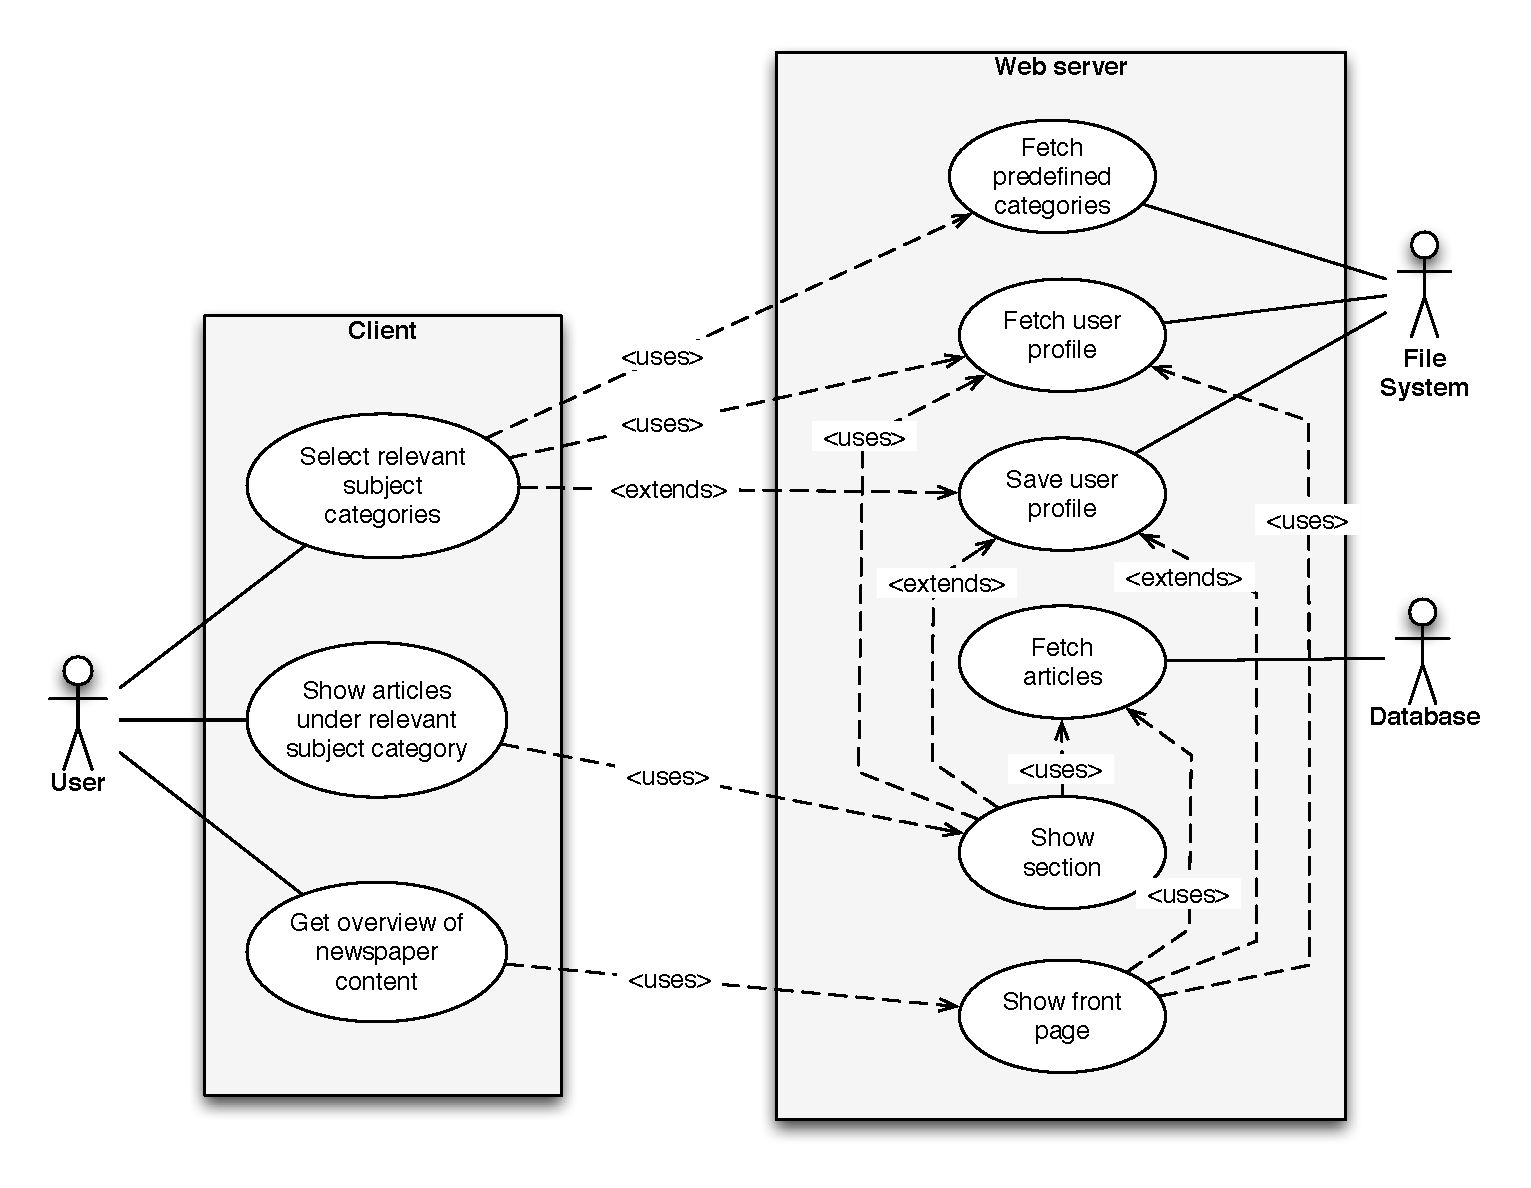
\includegraphics[width=\textwidth]{img/use-cases}}
	%\newlength{\graphicheight}
	\settoheight\graphicheight{\mygraphic}
	\mygraphic
	\marginnote{
	\begin{minipage}{\marginparwidth}
		\vspace{-\graphicheight}%
		\caption{The figure shows the overall use cases of the system and how the web server acts to accomplish them.}
		\label{fig:use-cases}
		\vspace{\graphicheight}
		\end{minipage}
	}
\end{figure}

The list of use cases shown in the figure are by no means a complete, but are selected because they have the closest relation to the user needs.

The user is able to select relevant subject categories to get an easy start with the application and the choices are thereafter saved to the user profile for later use. The user can select a subject category from the earlier chosen categories and browse articles from this subject within a section. If the user needs to get an overview of the content of the newspaper he can get the front page displayed, which contains a small collection of articles of most interest to the user.

In Figure~\ref{fig:sequence} is shown a sequence diagram of what the system does in order to display the front page (or a section), when the user opens the application.
%\sidecaptionfigure{\textwidth}{img/sequence}{The figure shows a sequence diagram from when the user chooses a subject category until he can read articles from this subject. \texttt{secNum} is the section number to display (the front page is section 0), \texttt{userId} is a string that identifies the user, \texttt{userPrefs} is the user preferences on the specific section and \texttt{articles} is the library of articles to compose the editorial mix of.}{fig:sequence}
\begin{figure}[h!tp]
	\centering
	
	\def\mygraphic{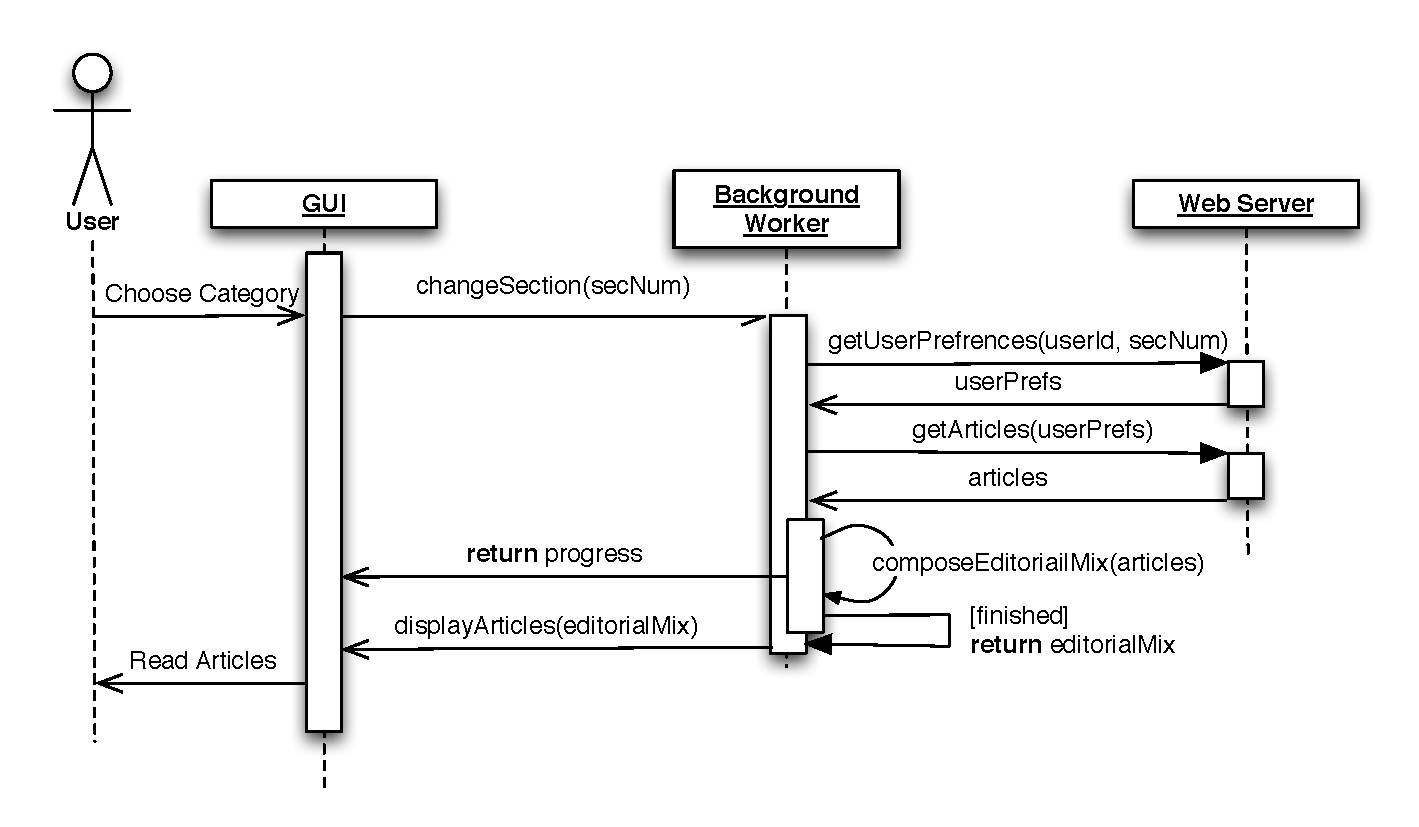
\includegraphics[width=\textwidth]{img/sequence}}
	\settoheight\graphicheight{\mygraphic}
	\mygraphic
	\marginnote{
	\begin{minipage}{\marginparwidth}
		\vspace{-\graphicheight}%
		\caption{The figure shows a sequence diagram from when the user chooses a subject category until he can read articles from this subject. \texttt{secNum} is the section number to display (the front page is section 0), \texttt{userId} is a string that identifies the user, \texttt{userPrefs} is the user preferences on the specific section and \texttt{articles} is the library of articles to compose the editorial mix of.}
		\label{fig:sequence}
		\vspace{\graphicheight}
		\end{minipage}
	}
\end{figure}
%\begin{figure}[h!tp]
%	\myfloatalign
%		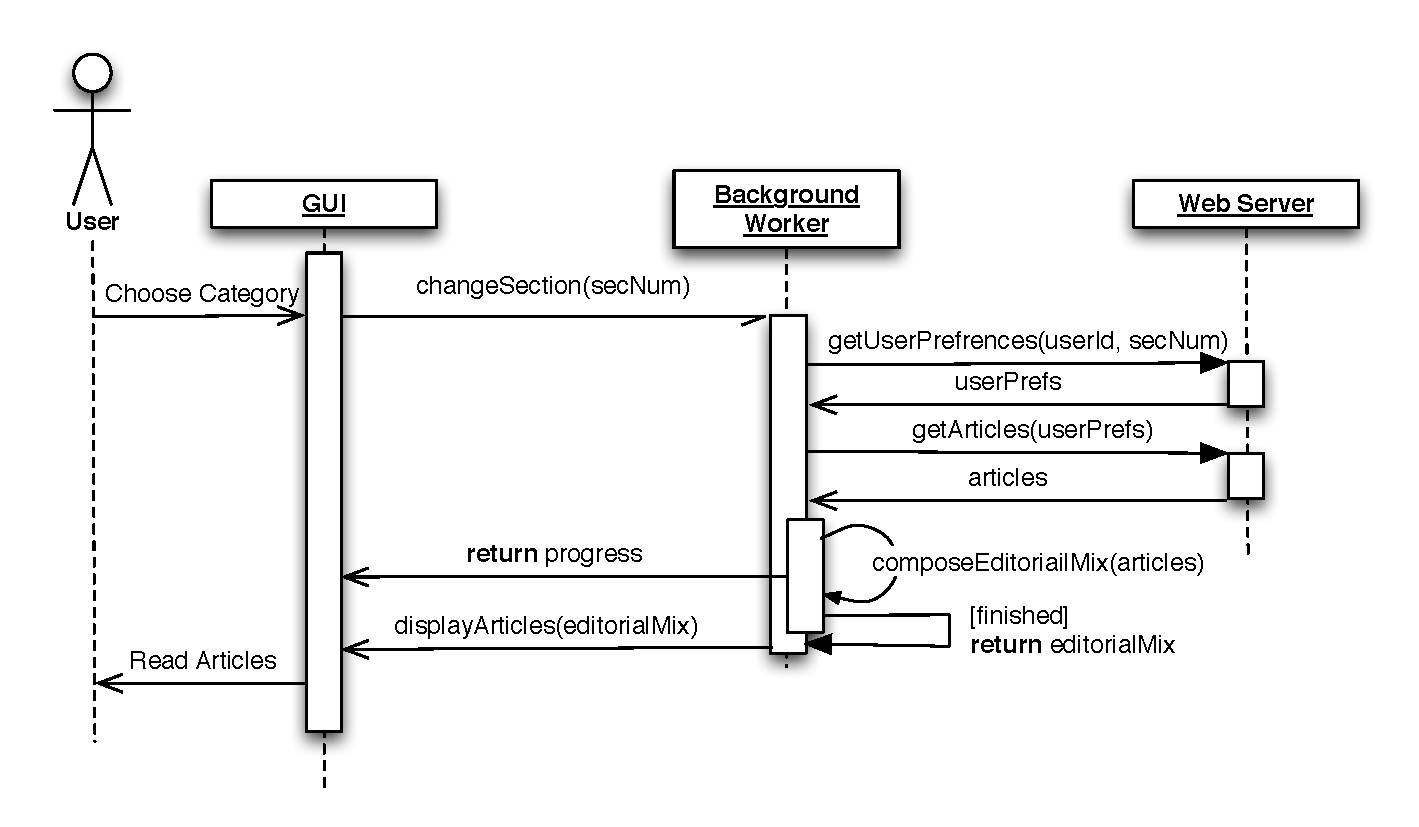
\includegraphics[width=\textwidth]{img/sequence}
%	\caption{The figure shows a sequence diagram from when the user chooses a subject category until he can read articles from this subject. \texttt{secNum} is the section number to display (the front page is section 0), \texttt{userId} is a string that identifies the user, \texttt{userPrefs} is the user preferences on the specific section and \texttt{articles} is the library of articles to compose the editorial mix of.}
%	\label{fig:sequence}
%\end{figure}

When the application is opened, or the application is changed to display a section, a background worker is initialised to compose its containing mix of articles. Of cause, if the mix of articles in a section, or front page, have already been computed, it does not need to recompute it. The background worker needs to get both the user preferences of the chosen category and article that potentially fit the user preferences. While worker computes the editorial mix it sends messages to the user interface about the progress. When it finishes the user interface is asked to display the articles.

\section{Requirements}
\subsection{Non-functional Requirements}
In the explored literature and the conducted tests users express some non-functional requirements. These are described in this section.

User needs states the requirement of having a clear overview of the content and as stated in \cite{FULLTEXT01.pdf}, this includes a clear marking of the beginning and the end of the articles and sections. This is obtained by both having a summery of the most interesting articles on the front page and by having a dropdown list of headlines in the top of section.

From the user needs it is also required that the system should be easily navigated and as stated by \cite{kristin_fredrik.pdf}, this should be through clickable sections, headlines and through paging. The layout, typography and design should be familiar to what is found in conventional newspapers, as stated by \cite{FULLTEXT01.pdf} and \cite{hcii2005_1004.pdf}. This is achieved by choosing a structure that resembles that of a newspaper and displaying content in balanced columns. It should be possible for the user to read the newspaper screen by screen, meaning that trailing text should be put into a new set of columns whenever it exceeds the screen, see Figure~\ref{fig:reading2} and \ref{fig:reading1}.

%\begin{figure}[h!tp]
%\myfloatalign
%\subfloat[Reading pattern where the user has to scroll in order to see the full length of the column.]{
%  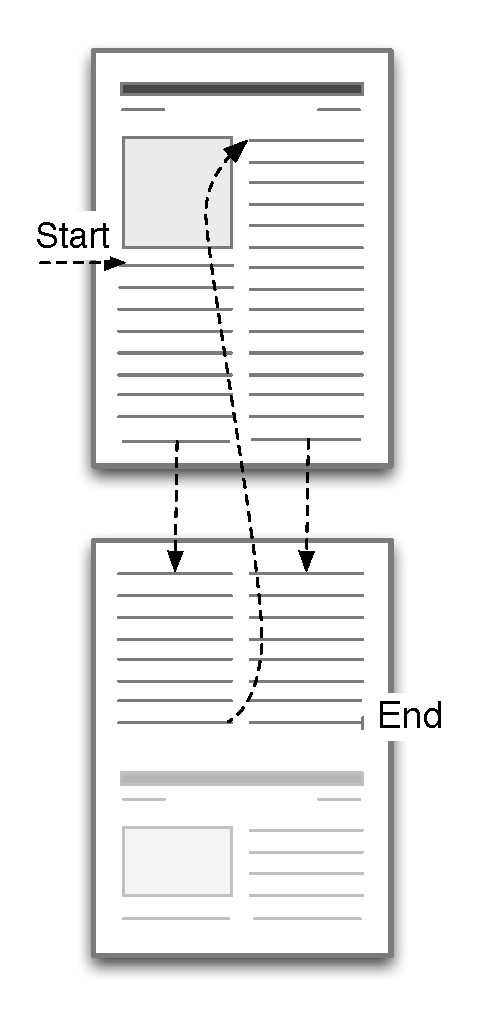
\includegraphics[width=.3\textwidth]{img/reading1}
%  \label{fig:reading1}
%} \qquad
%\subfloat[Reading pattern where the user can finish reading a whole page before scrolling to read the next.]{
%  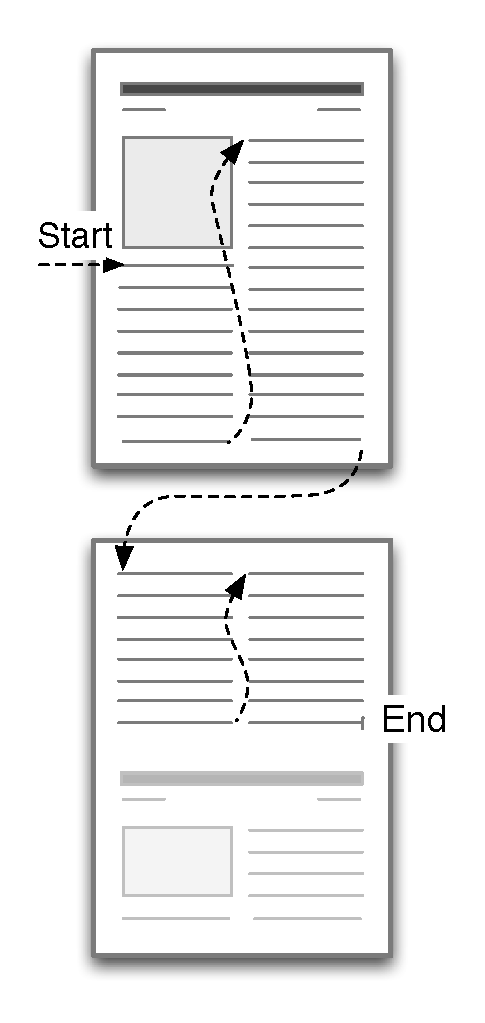
\includegraphics[width=.3\textwidth]{img/reading2}
%  \label{fig:reading2}
%}
%\caption{The figure shows two examples of reading patterns in a column based layout.}
%\label{fig:reading}
%\end{figure}

\begin{sidefigure}%
\centering%
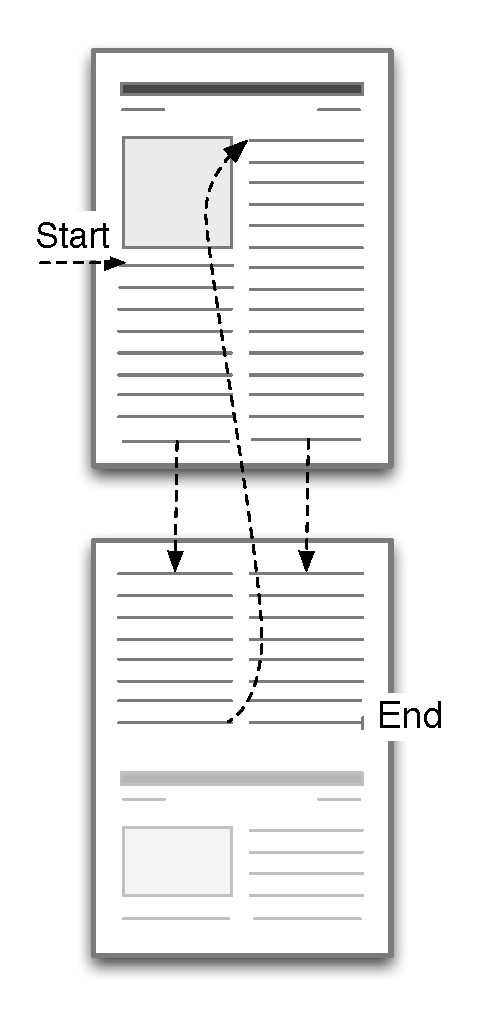
\includegraphics[width=\marginparwidth]{img/reading1} 
\caption{Reading pattern where the user has to scroll in order to see the full length of the column.}%
\label{fig:reading1}%
\end{sidefigure}

\begin{sidefigure}%
\centering%
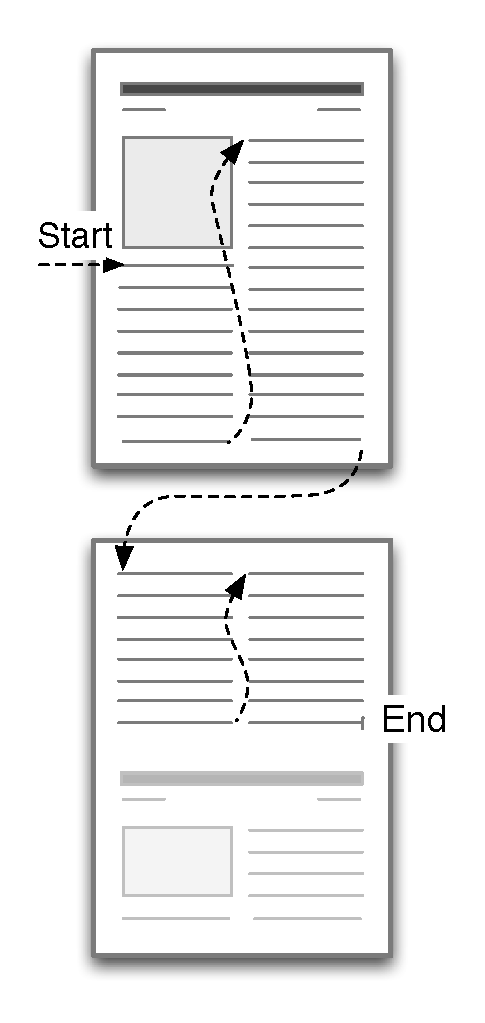
\includegraphics[width=\marginparwidth]{img/reading2} 
\caption{Reading pattern where the user can finish reading a whole page before scrolling to read the next.}%
\label{fig:reading2}%
\end{sidefigure}

\begin{itemize}
	\item Ease of use
	\item both general and personal news (collaborate filtering solves that some news are not received, but are universally interesting \cite{fulltext.pdf})
	
	\item both images and videos - test
	\item a good ratio of graphical and textual - test
	
	\item front page should give a good overview of the content - test
	\item ``news valuation, e.g. positioning of lead story'' \cite[p. 7]{FULLTEXT01.pdf}
	\item  mobility \cite[p. 7]{FULLTEXT01.pdf}
	\item  continuous updates \cite[p. 7]{FULLTEXT01.pdf}
	\item ``easy and intuitive navigation'' \cite[p. 7]{FULLTEXT01.pdf}
	\item add video and sound \cite[p. 7]{FULLTEXT01.pdf}
	\item incorporate social community and social networks
\end{itemize}

\subsection{Functional Requirements}
Some technical requirements have also been gathered from the explored literature.
\begin{itemize}
	\item ``open, turn pages, chose article, read and return'' \cite[p. 6]{FULLTEXT01.pdf}
	\item section headlines \cite[p. 6-7]{kristin_fredrik.pdf}
	\item article headlines
	\item article summaries / extracts \cite{fulltext.pdf}
	\item menu w. section headlines \cite[p. 8]{kristin_fredrik.pdf}
	\item page numbers \cite[p. 6-7]{kristin_fredrik.pdf}
	\item press ``like'' or key word based user profile (mark self or highlighted? right click to add): positive + negative list (keywords+categories \cite{10-1-1-19-5583}, \cite{fulltext.pdf} and \cite{gervasum2001ws.pdf})
	\item full screen display of article
	\item organise into personalised sections
	\item opens in front page view (summery of newspaper 8 articles) \cite[p. 8]{kristin_fredrik.pdf}
	\item adjust variables
	\item share directly (grey out the ones who have read it)
	\item comment
	\item see friends comments
	\item ``The presentation schema -- headline, abstract, and text, together with a relevance value with respect to the user profile -- rates the highest in terms of user satisfaction, and yet it is not the most frequent.'' \cite{Sections-categories-and-keywords-as-interest-specification-tools-for-personalised-news-services.pdf}
	\item  ability to search \cite[p. 7]{FULLTEXT01.pdf}
	\item Landscape + portrait \cite[p. 6-7]{kristin_fredrik.pdf}
	\item touch screen interaction \cite[p. 6-7]{kristin_fredrik.pdf}
	\item Functionality from online newspaper \cite{hcii2005_1004.pdf}
	\item Name of columnist \cite[p. 4]{gervasum2001ws.pdf}
	\item Transparency of implicit relevance feedback (see/modify current weights of categories) \cite[p. 7]{gervasum2001ws.pdf}
	\item dynamic short-term + static long-term user profile \cite{10-1-1-19-5583}, \cite{fulltext.pdf} and \cite{gervasum2001ws.pdf}
	\item relevance feedback \cite{10-1-1-19-5583}, \cite{fulltext.pdf} and \cite{gervasum2001ws.pdf}
\end{itemize}

%
%\subsection{Non-functional Requirements}
%\begin{itemize}
%	\item a good ratio between general and personal news
%	\item a good ratio between graphical and textual content
%	\item incorporation social network and community
%	\item a good reading flow
%\end{itemize}
%
%\subsection{Functional Requirements}
%Some technical requirements have also been gathered from the explored literature.
%\begin{itemize}
%	
%	\item easy navigation
%	\item contemplated typography and design
%	\item most interesting articles on the front page
%	\item opens in front page view (summery of newspaper few articles)
%	\item navigation through section headlines, article headlines and article summaries / excerpts
%	\item back page, funnies?
%	\item put in personalised sections
%	\item relevance value by article
%	\item menu with section headlines
%	\item page numbers
%	\item page turn
%	\item possibility of relevance feedback
%	\item keyword based user profile
%	\item ability to adjust preference variables
%	\item full screen display of article
%	\item columns should be divided to fit into one screen with possible images or videos
%	\item familiarity in design and layout from printed paper
%	\item news valuation, e.g.\ positioning of lead story
%	\item continuous updates
%	\item ability to search
%	\item video and sound
%	\item should be readable in both landscape and portrait
%	\item touch screen interaction
%	\item Functionality from online newspaper
%	\item Name of columnist
%	\item Transparency of implicit relevance feedback (see/modify current weights of categories)
%	\item dynamic short-term + static long-term user profile
%	\item relevance feedback
%\end{itemize}
%
\section{Delimitation}
The proposed design in chapter~\vref{ch:design} should of cause account for requirements, but there are some requirements that will not be implemented due to prioritisation and time limits

The initial approach involved computing the tf-idf similarity between documents and the user and the documents in between using the Python libraries for this \cite{NLTK}. This approach works on a bow (bag-of-words) with key words and weights representing a single item. The weight is computed by the number of occurrences in the provided text and a cosine distance determines the similarity. Python also provides an interface for working with WordNet -- a large lexical database of English words and their relationships in the form of different graphs. This opens the door to a more in-depth analysis of the optained news items. \cite{116262780379.pdf} presents an algorithm for enriching articles using WordNet's hypernym-graphs. A hypernym graph is generated by the top $20\%$ frequent keywords of an article and weighted by:
$$W(d, f) = 2 \cdot \frac{1}{1+e^{-0.125(d^3\frac{f}{TW})}}-0.5$$

Where $d$ stands for the node's depth in the graph (starting from root and moving downwards), $f$ is the frequency of appearance of the node to the multiple graph paths and $TW$ is the total number of words used to generate the hypernym graph.

In order to be able to work with hypernyms, the words must be converted to synsets. For each word there exists a synset for each use of the word, with the most frequently used first. Every synset is included at this point, but in a later stage this could be further focused by only using the top $n$. An analysis on how many percent of the words

\todo[inline]{Which design choices to focus on?}
Introduce columns and remove pages to introduce newspaper like layout

Do not focus on summaries -- out of scope, 

Support images only, not video -- can easily be introduced.

Not implement support for social networking, but included in the proposed design

Predefined categories is not a full list, but are of the most recurring in popular news sites.

\todo[inline]{In which period of time is an article relevant to a user? Maybe if it is still available, then it is still interesting -- new approaches or discussion about the subject might arise. How do we control that a news item is not missed? Keep index of what has been viewed in addition to what has been read.}


% section analysis (end)


%%!TEX root = thesis.tex
\chapter{Acquiring and Mining Data for Personalisation} % (fold)
\label{ch:theory}

% section results (end)


\cleardoublepage % Empty page before the start of the next part

%------------------------------------------------

\ctparttext{Discussing choices and presenting the solution.} % Text on the Part 1 page describing  the content in Part 1
\part{The Proposed Solution}

%!TEX root = ../thesis.tex
\chapter{Design} % (fold)
\label{ch:design1}
This section discusses different choices in the interface for a digital newspaper and how the application can provide the user with a personal editorial mix.

Before it is possible express the editorial mix problem formally the interface of the application must be described, because the constraints will have to make some assumptions about the application structure. The two following sections will describe the layout and typography of the application followed by the interaction with it.

\section{Layout and Typography}% (Interface Design)
\label{sec:layout_typography}
This section describes iterations of the design in terms of layout and typography and the preliminary work to base design choices on.

After the definition of the initial requirements was done the first prototype was developed. Its main features followed the requirements on turning pages, choosing an article, read it and returning to the overview of articles, see Figure~\ref{fig:prototype-iteration1}. And after a small preliminary survey it became clear, that a column-based layout showing full articles would be more attractive, and would provide a better opportunity to explore the editorial mix. With a column-based layout the digital newspaper would have more resemblance to conventional newspapers and therefore it was possible to apply some of the same principles of the editorial mix. This choice removed the paginated layout and instead introduced a scrollable layout to have enough space for the articles to fit in.
\begin{figure}%
%\centering%
\makebox[\textwidth][r]{% %%% as above; this time, the
%%% figures flushes from the left
\subfloat[Initial prototype layout with adjustable ratios between articles and a paginated interface of each section.\label{fig:prototype-iteration1}]%
	{\includegraphics[width=.37\largefigure]{img/prototype-iteration1}}%
	\qquad%
\subfloat[Second iteration of the prototype with an scrollable layout. Sections are placed beneath each other.\label{fig:prototype-iteration2}]%
	{\includegraphics[width=.37\largefigure]{img/prototype-iteration2}}%
}
\\
\makebox[\textwidth][r]{% %%% as above; this time, the
\subfloat[Third iteration of the prototype with a column-based and scrollable layout. Sections are placed beneath each other.\label{fig:prototype-iteration3-1}]%
	{\includegraphics[width=.37\largefigure]{img/prototype-iteration3-1}}%
	\qquad%
\subfloat[Third iteration of the prototype with a column-based and scrollable layout. Sections are placed beneath each other.\label{fig:prototype-iteration3-2}]%
	{\includegraphics[width=.37\largefigure]{img/prototype-iteration3-2}}%
}
\caption{The figure shows three iterations of the prototype layout.}%
\label{fig:prototype-iterations}%
\end{figure}
\clearpage
Figure~\ref{fig:prototype-iterations} shows three iterations of the prototype design, which were based on the derived requirements. The third iteration of the prototype (Figure~\ref{fig:prototype-iteration3-1} and~\ref{fig:prototype-iteration3-2}) was used as the foundation for user tests. The prototype consisted of the basic navigation between topic categories, i.e.\ sections, and articles. Navigational choices was made in order to present the general idea of the framework, but where more crucial choices on its uses have not yet been made. This was also to encourage the test subjects to talk about what uses they would have of the presented framework. However, they were also asked about the navigational structure and indeed some changes had to be done. A specification of the test can be found in Table~\ref{tab:test-description}.
\begin{table}[h!tp]
	\myfloatalign
	\marginnote{
		\begin{minipage}{\marginparwidth}
		\vspace{-100pt}
		\caption{Test Specification}
		\label{tab:test-description}
		\end{minipage}
	}
	\makebox[\textwidth][l]{
		\begin{tabularx}{.8\largefigure}{p{.15\largefigure}|p{.6\largefigure}}
		\toprule
			\textbf{Test subjects} & The test was conducted on a total of 7 test subjects of ages between 21-29, and of different sex and occupation.\\
		\midrule
			\textbf{Participants} & Each test was done with 1 test conductor and 1 test subject.\\
		\midrule
			\textbf{Materials} & An iPad with the application running and a computer to write notes on the test subject's statements and propositions.\\
		\midrule
			\textbf{Description} & The test subject was presented with the prototype layout seen in Figure~\ref{fig:prototype-iteration3-1} and~\ref{fig:prototype-iteration3-2}. The test was conducted as an informal qualitative talk with a basis in the test subject's interests in such a product. Transcripts from each test can be found at \url{http://lestrade.imm.dtu.dk/~s062596/data/test-transcripts.zip} and a summary of the results in section~\vref{sec:test_results}.\\
		\bottomrule
		\end{tabularx}
	}
\end{table}

The main points from the user test was that the newspaper should provide an overview of its contents and that it should be easy to navigate relevant new and archived articles. The users also wanted to provide relevance feedback on articles and wanted an indication of the relevance of the article. Moreover, that the newspaper should provide a good balance between images and textual content and that images should be as large as possible. It was also noted that white space in between articles was not a problem and that an article should be read screen by screen, even if it means dividing text into a new set of columns. Some of the test subjects pointed out that problems may arise if there is not room enough in the top menu, e.g.\ when in portrait mode and, as the test subjects specifically requested, this could be solved by introducing a carousel-like arrow buttons to scroll menu items, or even just using touch interactions. Moreover, the user should be able to read the newspaper screen by screen, meaning that trailing text should be put into a new set of columns whenever it exceeds the screen, see Figure~\ref{fig:reading}.
\begin{figure}[h!tp]
	%\vspace{-220pt}
	\myfloatalign%
	%\hspace{-17.8pt}
	\subfloat[Reading pattern where the user has to scroll in order to see the full length of the column.\label{fig:reading1}]{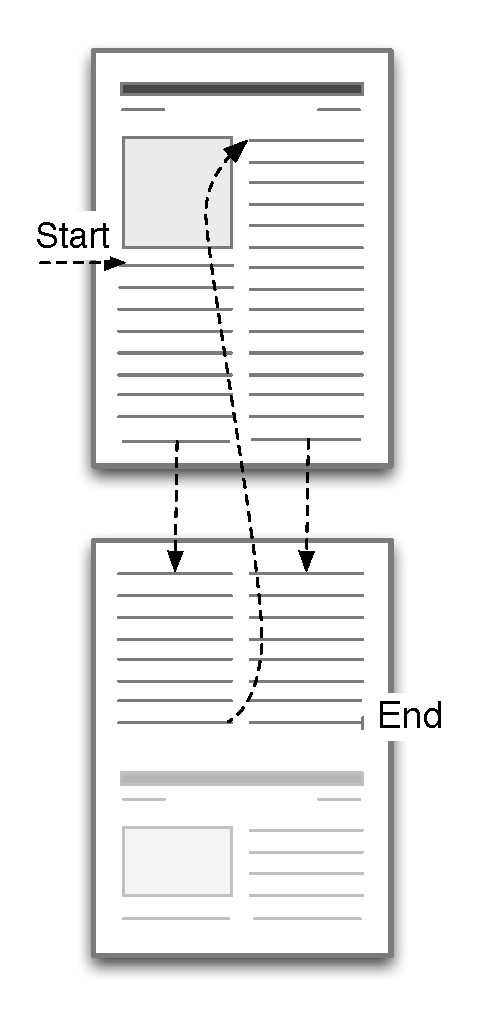
\includegraphics[width=\marginparwidth]{img/reading1}}
	\qquad
	%\hspace{-17.8pt}
	\subfloat[Reading pattern where the user can finish reading a whole page before scrolling to read the next.\label{fig:reading2}]{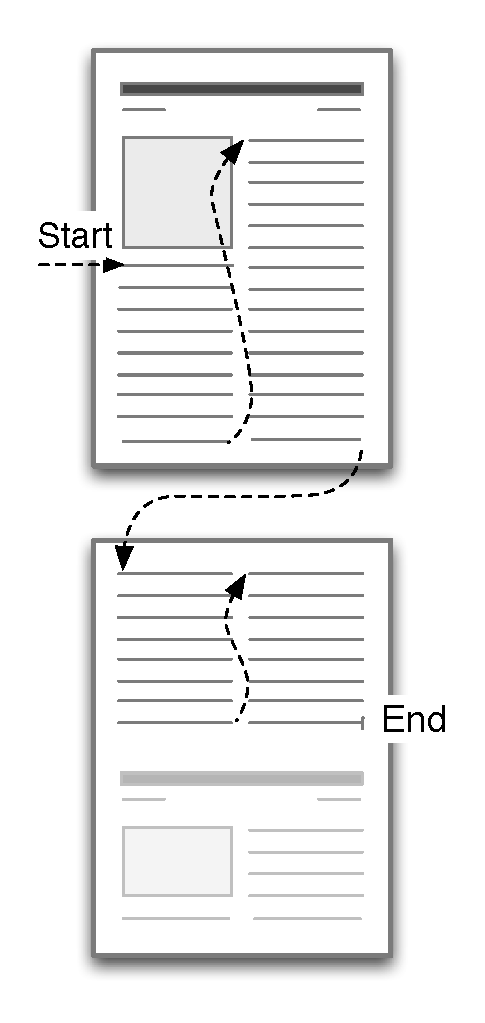
\includegraphics[width=\marginparwidth]{img/reading2}}
	\caption{The figure shows reading patterns of full length columns and columns divided into screen sized chunks.}%
	\label{fig:reading}
\end{figure}
%\begin{sidefigure}
%	%\vspace{-220pt}
%	\myfloatalign%
%	%\hspace{-17.8pt}
%	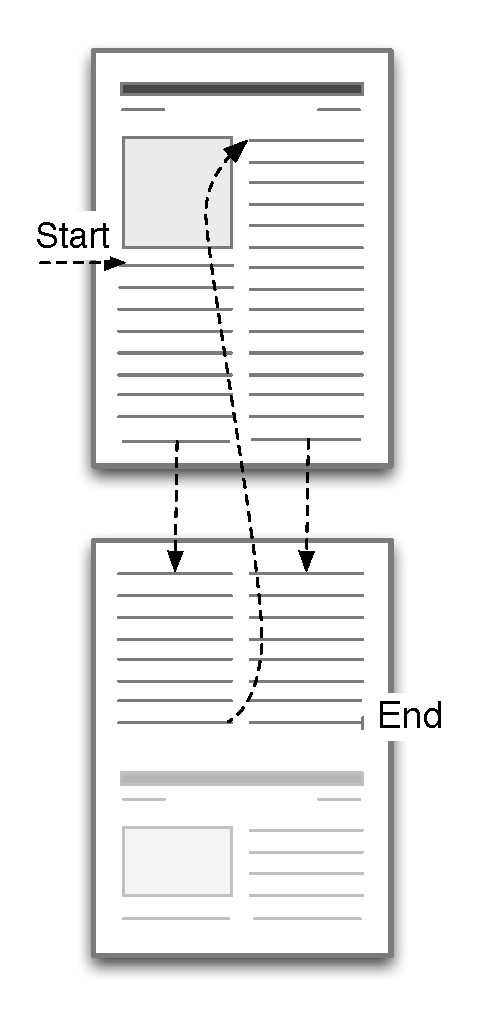
\includegraphics[width=\marginparwidth]{img/reading1}
%	\caption{Reading pattern where the user has to scroll in order to see the full length of the column.}
%	\label{fig:reading1}
%\end{sidefigure}
%\begin{sidefigure}
%	%\vspace{-220pt}
%	\myfloatalign%
%	%\hspace{-17.8pt}
%	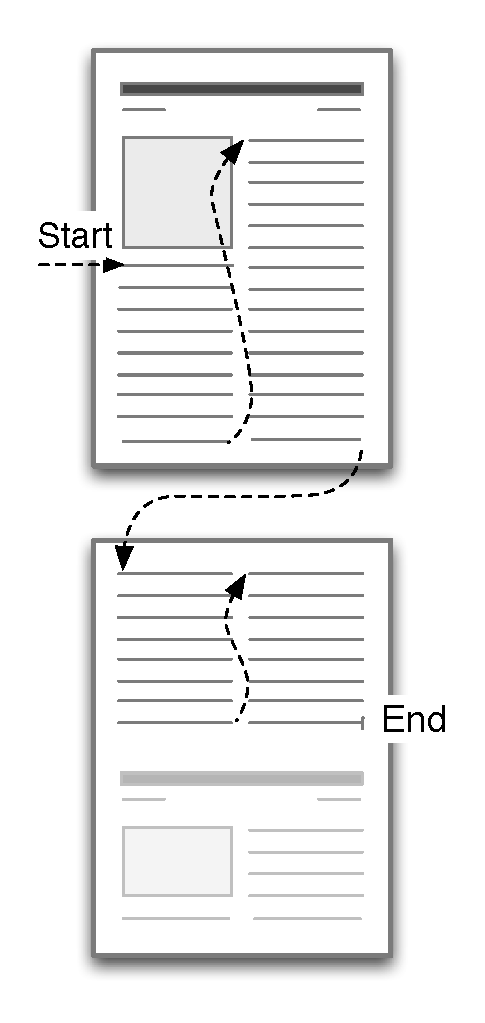
\includegraphics[width=\marginparwidth]{img/reading2}
%	\caption{Reading pattern where the user can finish reading a whole page before scrolling to read the next.}
%	\label{fig:reading2}
%\end{sidefigure}

Many of the test subjects played around with the text and expressed that it was good that the iPad could read the text out loud for them. One user in particular expressed that the application with some polish would provide a readable layout, easy navigation and a good overview of its content. She thought that this was the problems with \url{http://nyhederne.tv2.dk/}\sidenote{The website of a Danish news channel.}. No user expressed the need for any general news as presumed in the scenarios, only personalised news was of preference to the test subjects. They argued that if they wanted news of some kind, they would just create a section for it.

Even so \cite{fulltext.pdf} argues that common sense dictates some ``breaking'' articles to be universally interesting and that the problem of some user may not receive them\vspace{60pt}\sidenote{This is also known as the black sheep problem.}\vspace{-60pt} could be solved by collaborative filtering. Collaborative filtering is a good way to apply wisdom of the crowd to the application, which might make it stronger as the number users grows. Finally according to the user tests, it should be chosen from which period the articles should come from, as opposed to what was extracted from the scenarios and respondents from \cite{FULLTEXT01.pdf} which suggests that the paper should be continuously updated.

Based on the user feedback a new design was developed. It is seen in Figure~\ref{fig:mockups}.
\begin{figure}%
\myfloatalign
\makebox[\textwidth][l]{
	\subfloat%
			{\includegraphics[width=.43\largefigure]{img/mockup-landscape}}
		\qquad
	\subfloat%
		{\includegraphics[width=.33\largefigure]{img/mockup-portrait}}
}
\marginnote{
	%\begin{minipage}{\marginparwidth}
	\parbox{\marginparwidth}{
		%\vspace{-100pt}
		\caption{\\The figure shows mockups of the layout in landscape and portrait mode, respectively.}%
		\label{fig:mockups}%
		}
	%\end{minipage}
}
\end{figure}

The top menu from the prototypes is kept, but arrows are added to solve the problem of overflow if the items gets too numerous. The menu bar is given a dark colour to provide some visual contrast from content to functionality. In the new layout articles are shown in full and images are maximised. Rules of readability determines, as opposed to that on print, that small point size text work better with a sans-serif font \cite{Tidwell}. The neutral Helvetica has therefore been chosen as the body text, whereas the article headlines are the most important thing on the page, and therefore are supplied with the largest typeface. To provide them with further focus a serif font has been used. The section headers are assigned with a medium size, but wide, font because the user needs to navigate using this headline. However, the user already knows the name of the section (he has probably given it himself) and does therefore not necessarily need to read it -- just recognise it. On this basis the section headline is placed in a bar and supplied with the same light colour as the background. This makes them more neutral, but still easy to navigate using the bar. To relate the paratext with the section they are supplied with the same colour as the section bar. This should let the user associate the article with the topic of the section. Furthermore, the line that was on top of the articles (see Figure~\ref{fig:prototype-iteration3-2}) is moved to be beside it. This visually indicates when an article starts and ends. This will also aid to understand that the article continues if the article columns should be divided into screen sizes. Again the same colour as the section bar is used to set both the visual and contextual frame.

In the prototype the menu consisted of all the settings in a modal panel, but the test subjects wanted a division between visual tools, e.g.\ changing size of the font or colour scheme, and the content settings, i.e.\ the control of what each section should contain. The former is moved into a side menu with a button to access the latter, which is kept in a modal panel. This way the handy visual tools are only one interaction away, whilst the more complex settings are hidden away with two interactions. And the overview of article headlines in the section could be done as in Sublime Text 2\sidenote{Sublime Text 2 is a text editor for coding.}, see Figure~\ref{fig:sublime}
\begin{figure}[h!tp]
	\myfloatalign
	\includegraphics[width=.5\textwidth]{img/sublime}
	\marginnote{
		\begin{minipage}{\marginparwidth}
			\vspace{-220pt}
			\caption{The figure shows the overview plus detail function in Sublime Text 2.}
			\label{fig:sublime}
		\end{minipage}
	}
\end{figure}
This overview could be placed in the side menu and show a larger (and readable) scale of headlines and the user should be able to see the images further down in the newspaper.

\section{Interactions}% (Interface Design)
In Figure~\ref{fig:navigation} is the navigational structure of the application outlined. 
\begin{figure}[h!tp]
	\myfloatalign
		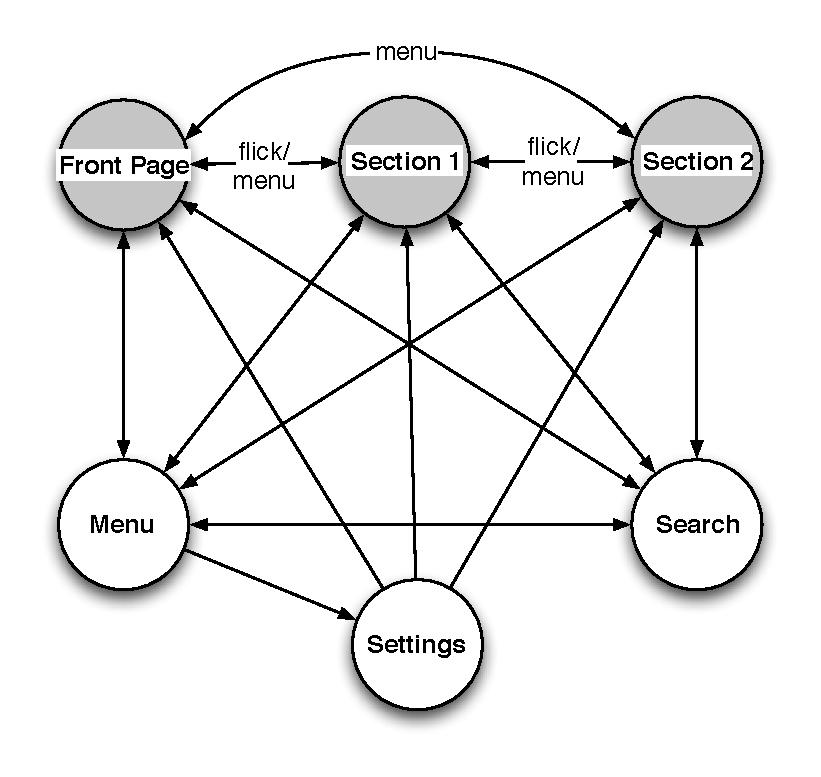
\includegraphics[width=.7\textwidth]{img/navigation}
	\marginnote{
		\begin{minipage}{\marginparwidth}
			\vspace{-240pt}
			\caption{The figure shows the navigational structure of the application. Arcs are navigational interactions and nodes are pages in the application.}
			\label{fig:navigation}
		\end{minipage}
	}
\end{figure}
The three sections (grey nodes) holds the contents of the newspaper, and can be extended with additional sections through the settings menu. That the top menu presents the items along side each other supports the fact that sections lay along side each other in the navigational space, i.e.\ it is possible to navigate to sections beside the current through the flick gesture (see Figure~\ref{fig:flick}).
% sections visually lie beside each other in the navigational space, i.e.\ the user can flick  the section and an animated transition slides the section out and the next in.
\begin{sidefigure}[h!tp]
	\myfloatalign
	%\vspace{200pt}
	\includegraphics[width=\marginparwidth]{img/flick}
	\caption{Touch gesture: Quickly brush surface with fingertip.}
	\label{fig:flick}
\end{sidefigure}

An animated transition could visually supports this structure by sliding the section out and the next in (same direction as the gesture). It is, however, still possible to directly reach any of the section through the top menu. Because the top menu is visible at all times except when in the settings menu, it is possible to go directly to any of the sections and do a search anywhere from the application, except of course from the settings menu. This means that the application is very interconnected and since the settings menu is meant to be used rarely the extra navigational step does not matter. The settings menu should only be used the first time the user opens the application to adjust the basic settings and then afterwards only to correct if the application does not comply with the user preferences, or when the super user wants to adjust the settings. In a perfect world the user would never have to open the settings menu to adjust anything, only observe while the application learns the user interests and delivers what is expected.

When the user is at first presented with the application he should have as a direct path as possible leading to actually reading articles, which is of main user needs. He is presented with a form to make choices about the contents of the newspaper. The application provides the possibility for choosing whether the front page should be visible or not. This functionality is given to the user that would rather just have his sections and no front page. After this the user can choose the topic for the first section from a list of predefined topics. If the topic he is looking for is not in the list he can choose to fill out some keywords to cover his interests. After this he can provide it with a name for the section and choose to add another section or save his user profile. It is also possible for him to choose how many articles he would like in each section, including the front page. Figure~\vref{fig:mockup-form} shows a mockup of the settings menu.
\begin{figure}[h!tp]
	\myfloatalign
		\includegraphics[width=.45\textwidth]{img/mockup-form}
	\marginnote{
		\begin{minipage}{\marginparwidth}
			\vspace{-300pt}
			\caption{The figure shows mockup of the form that constitutes the settings menu.}
			\label{fig:mockup-form}
		\end{minipage}
	}
\end{figure}
%\todo[inline]{Heuristics evaluering?}

Finally, it is important to state that users tend to play more with the screen when reading on tablet computers. Therefore the application should support selection of text and as from the text it should be possible to get it read out loud. This way articles can also become audio books.

To be able to solve the editorial mix problem using CP it must be introduced and the presented constraints must be translated to logical constraints. This is done in the following chapter.

\chapter{Constraint Programming}
\label{ch:design2}
The purpose of this chapter is to introduce the reader shortly to CP and afterwards define the problem as a COP. Different possibilities for implementation exists and this chapter will discuss these choices and conclude with a choice of algorithm.

\section{Constraint Programming and Personalisation}
%\todo[inline]{Om skriv til mere pædagogisk og forståeligt. Argumentér for at CP er god til kombinatoriske problemer.}
To be able to use CP to solve the editorial mix as a personalisation problem, it is necessary to define which problems CP works with. Constraint Satisfaction Problems (CSPs) and Constraint Optimisation Problems (COPs) are the two types of problems CP can be used to solve. The following descriptions of CSPs and COPs have been modified to fit personalisation problems from the original definitions provided by \shortcite{AIRussell} and~\cite{CPApt}.

A Constraint Satisfaction Problem is defined by the 4-tuple $(\mathcal{V}, \mathcal{X}, \mathcal{D}, \mathcal{C})$, where $\mathcal{V}$ is the set of values, $\mathcal{X}$ is the set of variables, $\mathcal{D}$ is the corresponding set of domains and $\mathcal{C}$ is the set of constraints on the variables.

Each variable has a corresponding domain and each domain has sub-domains corresponding to the attribute of each variable. A value also has a set of attributes, but they may extend the variables set of attributes. However, if a variable is assigned, the variable's attributes should reflect that of its assigned value\vspace{-40pt}\sidenote{Others do not consider representation of values because they in their case only consist of simple integer, real or boolean values.}\vspace{40pt}\hspace{-.6em}. Unlike \shortcite{AIRussell} and~\cite{CPApt} a constraint is here defined as a function on specific variables returning a boolean value.

Therefore the tuple of $u$ values with $w$ attributes, $n$ variables with $m$ attributes and $p$ constraints, where the $i$th constraint is defined on $s_i$ variables, can be expanded to:
%\hspace{-\marginparwidth}
%\hspace{-\marginparsep}
%\begin{minipage}{.8\largefigure}
\begin{align}
\begin{pmatrix}\vspace{3pt}
\mathcal{V}:&
	\begin{Bmatrix}
		v_1:
		\begin{pmatrix}
			v_1.a_1\\
			\vdots\\
			v_1.a_w\\
		\end{pmatrix}
		, \ldots,
		v_u:
		\begin{pmatrix}
			v_u.a_1\\
			\vdots\\
			v_u.a_w\\
		\end{pmatrix}
	\end{Bmatrix},\\\hspace{3pt}
	\mathcal{X}:&
	\begin{Bmatrix}
		x_1:
		\begin{pmatrix}
			x_1.a_1\\
			\vdots\\
			x_1.a_m\\
		\end{pmatrix}
		, \ldots,
		x_n:
		\begin{pmatrix}
			x_n.a_1\\
			\vdots\\
			x_n.a_m\\
		\end{pmatrix}
	\end{Bmatrix},\\\hspace{3pt}
	\mathcal{D}:&
	\begin{Bmatrix}
		d_1:
		\begin{pmatrix}
			d_1.a_1\\
			\vdots\\
			d_1.a_m\\
		\end{pmatrix}
		, \ldots,
		d_n:
		\begin{pmatrix}
			d_n.a_1\\
			\vdots\\
			d_n.a_m\\
		\end{pmatrix}
	\end{Bmatrix},\vspace{6pt}\\
	\mathcal{C}:&
	\begin{Bmatrix}
		c_1: func(x_{(1,1)}, \ldots,x_{(1,s_1)}) \rightarrow \mathbb{B},\\
		\vdots\\
		c_p: func(x_{(p,1)}, \ldots,x_{(p,s_p)}) \rightarrow \mathbb{B}
	\end{Bmatrix}
\end{pmatrix}
\label{eq:problem_spec}
\end{align}
%\vspace{6pt}
%\end{minipage}
Where $\mathbb{B}$ is either \texttt{true} or \texttt{false}.

A CSP is a special case of a Constraint Optimisation Problem (COP) and a COP is defined by the 5-tuple $(\mathcal{V}, \mathcal{X}, \mathcal{D}, \mathcal{C}, \mathcal{O})$, where the first four elements are defined as in a CSP and $\mathcal{O}$ is a set of objective (or cost) functions on variables, that determines the quality of a current state. The set of objective functions can be described with the same structure as constraints in CSPs and can be expanded as follows with $q$ constraints, where the $i$th function is defined on $t_i$ variables.
\begin{align}
	\mathcal{O}:&
	\begin{Bmatrix}
		o_1: func(x_{(1,1)}, \ldots,x_{(1,t_1)}) \rightarrow \mathbb{R},\\
		\vdots\\
		o_q: func(x_{(q,1)}, \ldots,x_{(q,t_q)}) \rightarrow \mathbb{R}
		%o_1 : func(x_i, \cdots,x_{i+t}) \rightarrow \mathbb{R}, \cdots, o_l : func(x_j, \cdots,x_{j+u}) \rightarrow \mathbb{R}
	\end{Bmatrix}
	\label{eq:objective}
\end{align}

Where $\mathbb{R}$ is the set of real numbers.

Satisfaction (or regular) constraints are also called hard constraints and objective functions are called soft constraints because a solution can be found if all hard constraints are satisfied, whereas an optimal assignment is enough to satisfy objective functions.

Finally, a constraint on a single variable is called an unary constraint, a constraint on two variables is called a binary constraint and a constraint on three or more variables is called a global constraint.

\section{Problem Representation}
\label{sec:problem_representation}
The division of rules between the front page and the section can be kept in the problem representation, which will, as we will see later, be the source for the possibility of incorporating lazy loading of each section. This section will therefore present a general problem specification for a section, which can be used in every section and on the front page, with varying constraints. Also, the front page will throughout this chapter be referred to as a section, and specifically as section $0$.

The set of values, $\mathcal{V}$, from equation~\ref{eq:problem_spec} in the problem is represented by a library of currently available articles and the set of variables, $\mathcal{X}$, is represented by the available positions in the section. Each variable can then be assigned a value in the form of a specific article and a solution has been found, when a complete assignment satisfies all constraints. An article consists of a set of attributes, e.g.\ a date, the number of words in the article and a number indicating a relevance. Constraints are defined on variables and through them bound to their specific places in the section.

In the following the constraints presented in section~\vref{sec:analysis_mix} will be formulated as logical constraints divided into general constraints for all sections and specific constraints for the front page and other sections, respectively. Constraints defined on variables with letters $a$ and $b$, i.e.\ $x_a$ and $x_b$, means that the constraint is defined for every combination of variables from the problem. Hard constraints (equation~\ref{eq:problem_spec}) returns whether it is satisfied and preference constraints (equation~\ref{eq:objective}) returns a violation, where $0$ means not violated.

\subsection*{General Unary Constraints}
\vspace{-30pt}
\begin{align}
	\begin{Bmatrix}
		\texttt{time-frame}(x_a) &\rightarrow& x_a.date >= today-7,\\
		\texttt{featured-space}(x_a) &\rightarrow& x_a.featured = \texttt{false}\ \vee\\
			&&x_a.columns = 2\ \vee\\
			&&x_a.columns = 3,\\
		\texttt{nonfeatured-space}(x_a) &\rightarrow& x_a.featured = \texttt{true}\ \vee\\
			&&x_a.columns = 1\ \vee\\
			&&x_a.columns = 2,\\
		\texttt{featured-image}(x_a) &\rightarrow& x_a.featured = \texttt{false}\ \vee\\
			&&x_a.has\_image = \texttt{false}
	\end{Bmatrix}
	\label{eq:general_unary}
\end{align}
%\texttt{\textbf{if}}(
%)\\
%&&\texttt{ \textbf{return} } 0 \texttt{ \textbf{else return} } 1

Where $today$ is variable that holds the current date. The \texttt{time-frame} constraint is a part of the temporal aspect of the problem. It is set to include articles from a week ago, but can of course be adjusted. As the layout is defined in 2 and 3 columns the \texttt{featured-space} constraint is satisfied only when the article fills out 2 or three 3 columns. Likewise with the \texttt{nonfeatured-space} which is only satisfied with articles that fills 1 or 2 columns. These two constraints are a part of the spatial aspect of the problem. \texttt{featured-image} is a constraint, to control that a featured article should have an image. These final three constraints could be used as they are, but could also function as assignments along with a calculation of the relevance to base the rest of the constriants on, i.e.\ to determine that a featured article is an article with many words, has an image and has a lot of relevance; otherwise it is not.
%$n$ is the number of positions and therefore variables, in the section and

\subsection*{General Binary Constraints}
\hspace{-40pt}
\begin{minipage}{.9\largefigure}
\vspace{-30pt}
\begin{align}
%\hspace{-60pt}
	\begin{Bmatrix}
		\texttt{featured-adj}(x_a, x_b) &\rightarrow& \texttt{not adjacent}(x_a,x_b)\ \vee\\
			&&(x_a.featured = \texttt{false}\ \wedge\\
			&&x_b.featured = \texttt{false})\ \vee\\
			&&(x_a.featured = \texttt{true}\ \wedge\\
			&&x_b.featured = \texttt{false})\ \vee\\
			&&(x_a.featured = \texttt{false}\ \wedge\\
			&&x_b.featured = \texttt{true}),\\
		\texttt{featured-pos}(x_a, x_b) &\rightarrow& \texttt{not adjacent}(x_a,x_b)\ \vee\\
			&&(x_a.featured = \texttt{false}\ \wedge\\
			&&x_b.featured = \texttt{false})\ \vee\\
			&&(x_a.featured = \texttt{true}\ \wedge\\
			&&x_a.position > x_b.position)\ \vee\\
			&&(x_b.featured = \texttt{true}\ \wedge\\
			&&x_b.position > x_a.position),\\
		\texttt{adj-subj}(x_a, x_b) &\rightarrow& \texttt{\textbf{if}}(\texttt{not adjacent}(x_a,x_b))\\
			&&\texttt{\textbf{return} max}(0,\\
			&&64 \cdot \texttt{similarity}(x_a,x_b)^2\\
			&& - 64 \cdot \texttt{similarity}(x_a,x_b)\\
			&& + 15.36)\\
			&&\texttt{\textbf{else return }}0
	\end{Bmatrix}
\end{align}
\end{minipage}

Where $\texttt{max(number,\ number)}$ is a function that returns the maximum of the given numbers and $\texttt{similarity}(variable,\ variable)$ is a function that returns the mutual similarity between the values of two given variables. These general binary constraints control most of the editorial mix, because they express that two featured articles should not be placed adjacent to each other, that featured articles should be placed higher than its adjacent non-featured articles and that adjacent articles should have the same subject. The latter is a preference constraint because some uncertainty is introduced when controlling that two articles should have the same subject. That articles have the same subject can approximately be determined by how similar they are to each other, i.e.\ if the articles are much too similar they could be articles on the same story, and if they differ too much, they may be on a different subject. However, in between should roughly determine that the articles are on the same or a similar subject, which is what is needed. In the \texttt{adj-subj} constraint this is done by returning a violation based on the parabolic function seen in Figure~\ref{fig:curve}.
\begin{figure}%
\myfloatalign
\includegraphics[width=.45\textwidth]{img/curve}
\marginnote{
	\begin{minipage}{\marginparwidth}
		\vspace{-200pt}
		\caption{Plot of $10 x^2 - 14 x +4.8$.}%
		\label{fig:curve}%
	\end{minipage}
	}
\end{figure}

The function was chosen to express the needed violation if articles did not match the desired similarity. If the similarity of the two articles are below $0.6$ or above $0.8$, then its distance to this point will determine its violation by the parabolic function. These numbers are of course adjustable and will vary according to the selected similarity function, but are given to show a more expressive example. These constraints are part of the relational aspect of the problem.
%(-1.4a+sqrt((-1.4a)^2-4a(-0.1+0.49a)))/(2a)=0.8
%(-14/225+sqrt((-14/225)^2-4*2/45*137/1125))/(4/45)
\subsection*{General Global Constraints}
\vspace{-30pt}
\makebox[\textwidth][r]{
\begin{minipage}{.9\largefigure}
\begin{align}
	\begin{Bmatrix}
		\texttt{all-diff}(x_1,\ldots,x_n) &\rightarrow& \bigwedge\limits_{i=1,\dots,n}\bigwedge\limits_{j=1,\dots,n}\ \texttt{similarity}(x_i,x_j) < 0.9
	\end{Bmatrix}
\end{align}
\end{minipage}
}
Where $n$ is the number of positions and therefore variables, in the section. The final of the general functions determines that every article must be different. In the constraint this is expressed by checking if the similarity between the articles is too high, it could also be done by just checking the internal application ID of the article, but this might introduce more of the same story, but from different content providers. This is also a part of the relational aspect of the problem.
%\begin{itemize}\itemdist
%%\subsubection{Unary}
%	\item An articles should be within a given time frame
%	\item A featured articles should be allowed to take up more space
%	\item A featured articles should be accompanied by an image
%	\item A non-featured article should take up less space
%%\subsubection{Binary}
%	\item A featured article should be adjacent to non-featured articles
%	\item A featured should have a higher position than its adjacent non-featured articles
%\item Articles should be grouped into subjects
%%\subsubection{Global}
%	\item All articles should be different
%\end{itemize}

\subsection*{Front Page Constraints}
%\makebox[\textwidth][l]{
\hspace{-30pt}
\begin{minipage}{.9\largefigure}
\vspace{-30pt}
\begin{align}
	\begin{Bmatrix}
		\texttt{main-stories}(x_a) &\rightarrow& \bigvee\limits_{i=1,\dots,g}\ \texttt{relevance}(x_a,i) >= 0.75,\\
		\texttt{nonfeatured-image}(x_a) &\rightarrow& \texttt{\textbf{if}}(x_a.has\_image) \texttt{\textbf{ return }}0\\
		&&\texttt{\textbf{else return }}1
	\end{Bmatrix}
\end{align}
\end{minipage}
%}

Where $g$ is number of sections and $\texttt{relevance}(variable,\ section\ number)$ returns the relevance of the given variable in the given section number. The former constraint expresses the need for only articles of high relevance on the front page. This is therefore also a part of the relational aspect of the problem. The latter expresses that non-featured articles preferably also should have images on the front page.
%\begin{itemize}\itemdist
%%\subsubection{Unary}
%	\item An article should have a very high level of relevance to at least one of the section topics
%	\item Most or every non-featured article should be accompanied by an image
%%\subsubection{Binary}
%%\subsubection{Global}
%\end{itemize}

\subsection*{Section Constraints}
\hspace{-40pt}
\begin{minipage}{.9\largefigure}
\vspace{-30pt}
\begin{align}
	\begin{Bmatrix}
		\texttt{topic}(x_a) &\rightarrow& \texttt{relevance}(x_a,k) >= 0.65,\\
		%\texttt{nonfeatured-image}(x_a) &\rightarrow& x_a.has\_image = \texttt{false},\\
		\texttt{fp-article}(x_1,\dots,x_n) &\rightarrow& \bigvee\limits_{i=1,\dots,n}\bigwedge\limits_{j=1,\dots,m}\ x_i.id = a_j.id,\\
		\texttt{image}(x_t, x_{t+1}, x_{t+2}, x_{t+3}) &\rightarrow& \texttt{\textbf{if}}(\bigvee\limits_{i=t,\dots,t+3}\ x_i.has\_image)\\
		&& \texttt{\textbf{ return }}0\texttt{\textbf{ else return }}1
	\end{Bmatrix}
	\label{eq:section_constraints}
\end{align}
\end{minipage}

Where $k$ is the current section number, $a_1,\dots,a_m$ is a list of articles from the front page that should be contained in this section and $x_t$ are variables where $t$ fulfils the equation $(t-1)\ \texttt{\textbf{mod}}\ 3 = 0$. In other words, it is defined for every fourth variable. The first section constraints controls that articles should be relevant to the topic, which is therefore a relational part of the problem. The two latter controls that this section contains all necessary articles from the front page and that at least every fourth article should hold images.

It is worth noting that there is no constraint defining combinations of attributes to make up articles. In a classical sense the CP could solve this problem, but would probably end up with a combination of attributes for each article, that would solve the problem perfectly, but is impossible to find in the library. The classical sense of CP is therefore in some cases more hypothetical, meaning that it would solve the problem in terms of numbers and boolean values, but does not reflect the real world. This approach works well for school examples like a planning problem or the well-known $n$-Queens problem\sidenote{A classic CP problem: Place $n$ queens on a $n \times n$ chessboard, so no queen is attacked.} and if one were to follow the classical sense of CP one would have to define constraints expressing legal combinations of attributes. This will, however, not be an optimised solution as the library of articles potentially could be very big in this problem and would require a constraint for each, which would increase the problem size and therefore the time to solve it significantly. A small example of this is an automatic playlist generator written in Prolog, that defines a whole music library and generates a playlist based on some constraints\sidenote{The library can be downloaded here: \url{http://lestrade.imm.dtu.dk/~s062596/data/PrologAPG.zip}.}. Running this program one realises that this is not very efficient for a library of about $5000$ songs. Therefore a novel approach is proposed. Instead of defining constraints based on the library of articles values are assigned based on look-ups in the library, which thereby introduces implicit constraints of attribute constraints, i.e.\ it is never possible for the system to find a combination of attributes, which is not found in the library, because they are taken from the library. This will also introduce some randomness to the compositions, which is often sought in real world problems.
%\todo[inline]{I do not have a reference for this last part. Does it matter? what about combinatorial personalisation problems?}

Following the classical sense of CP the variables could be viewed as ``mega-variables'' and the combination of attributes could be defined as a sub-problem. The combination of attributes found in the library could be expressed as a big logical OR constraint. Whenever a value for a variable in the super-problem is needed the sub-problem could be solved. This structure of the sub-problem will incrementally look through the library returning the first value combination of attributes that satisfies the big logical OR constraint. This is done every time the super-problem needs a value, which is not an optimal solution.

The presented constraints are more or less simply translated from the presented textual constraints into logical functions and luckily only few contains multiple or every variable in the problem. It is in many cases profitable to choose a different representation of the problem if constraints builds on multiple variables. This can be done e.g\ by a tree decomposition or a reduction of the constraints to binary constraints. To compose the tree decomposition, first the constraint graph\sidenote{A constraint graph is a graph where vertices are variables of the problem and their links are the constraints that binds them.} needs to be considered. In this problem a complete graph of all variables will emerge, as it contains constraints that holds every variable. The tree decomposition is done by dividing the problem into sub-problems and again viewing them as ``mega-variables'' with their set of solutions as their respective domains, so the outermost problem becomes a tree. \shortcite{AIRussell} states that this works well if no sub-problem is too large, but for a complete graph of $n$ variables the tree decomposition will become a problem of $n-1$ sub-problems each with $n-1$ variables, which is not very efficient. As each sub-problem can be solved independently the decomposition could be done continuously until small enough problems emerge. However, the time is of course dependent on the branching factor of the tree, so this is not efficient either. Reduction of constraints to binary constraints can be done by introducing new variables, with constraints that defines the relation to this and old variables in the new problem. \shortcite{AIRussell} however argues that it is possible to design special-purpose inference algorithms that only handles global constraints and in practice this can be done by counting the number of variables the constraint is defined for and then deciding how to handle it.

\section{Choice of Algorithm}
Because the problem is a fixed budget computation problem, in that the user should not have to wait too long for a solution, it is worthwhile exploring the algorithm choices of the solution.

Several algorithms exists to solve CSPs and many of them can be converted to work on COPs. A depth-first search using \textsc{Backtracking} can e.g.\ be used. The search continues with a descendant spanning the whole tree, which is independently viewed as a new CSP. The search backtracks to the parent node, whenever an empty domain is encountered. The algorithm stops with the first assignment that satisfies the CSP if a single solution or inconsistency is sought. Because no information, other than that given in the problem formulation, is used to solve the problem it is a uniformed search and therefore not expected to perform very well~\shortcite[p. 81]{AIRussell}.
%, but . In the papers \cite{LSVossen} and \cite{lunoe} are argumentations for using the $Min-Conflicts$ algorithm is found

With the use of heuristics the search can be improved. An example of this is the \textsc{branch and bound} search which work on COPs, but can handle CSPs as well. The branch and bound heuristic bounds the search by an objective function, that returns the current best assignment. States after a worse assignment is encountered are therefore not considered. Another example of a heuristic function is the \emph{most-constrained-variable} (MCV) heuristic. This function always selects the variable that appears in the largest number of constraints, to be assigned next. When used with backtracking, the performance can be greatly improved~\cite[pp. 337]{CPApt}.

\emph{Constraint Propagation} is another type of heuristic. Where the branch and bound heuristic is concerned with which variable to select, constraint propagation is concerned with the implications of the assignment of a variable. This means that if the assignment of a variable removes the possibility of some values to others in the solution, the values are removed from these domains. An example of this is \emph{arc consistency}. If every constraint is represented by an arc, like in the constraint graph, but directed, arc consistency is when there for every value exists some value that it is consistent with. Arc consistency can be applied multiple times to obtain \textit{path consistency} and until no inconsistency is left, which is the property of the \textsc{MAC} (Maintaining Arc Consistency) algorithm.

\textsc{forward checking} uses propagation whenever a variable is assigned to a value to detect inconsistency. It does, however, not detect for new inconsistencies after the removal of values.
%The worst-case time for \textsc{MAC} is $O(cd^3)$ for $c$ binary constraints and $d$ values in a problem as described in~\cite[p. 210+218]{AIRussell 1(146)}. Even so will, \textsc{MAC}, still not find every inconsistency (\cite[p. 150]{CPApt} and \cite[p. 211]{AIRussell 1(147)}).
%The enumeration and Constraint Propagation heuristics are both direct properties of the \textsc{forward checking} search.

Finally there is the \textsc{Min-Conflicts} algorithm. It is the result of the application of \textit{local search} to CSPs. It uses the min-conflicts heuristic, which chooses the value that results in a minimum number of conflicts. The algorithm is shown in Figure~\ref{fig:minConflicts}.
\clearpage
\begin{figure}[ht!p]
	%\hspace{-40pt}
	\newsavebox{\minconflictsbox}
	\begin{lrbox}{\minconflictsbox}
	\begin{minipage}{.8\largefigure}
		\vspace{-5pt}
		\begin{codebox}
\zi \proc{Min-Conflicts}($csp$, $max\_steps$) \kw{returns} a solution or failure
    \Indentmore
\zi \kw{inputs:}
    \Indentmore
    \zi $csp$, a constraint satisfaction problem
    \zi $max\_steps$, the number of steps allowed before giving up \End
\zi $current \leftarrow$ an initial complete assignment for $csp$
    \zi \For $i = 1$ to $max\_steps$ \kw{do} \Do
    \zi     \If $current$ is not a solution for $csp$
    \zi     \Then \Return $current$ \End
    \zi     $var \leftarrow$ a randomly chosen,
    \zi     \hspace{28pt} conflicted variable from \proc{Variables[$csp$]}
    \zi     $value \leftarrow$ the value $v$,
    \zi     \hspace{37pt} that minimises \proc{Conflicts($var$, $v$, $current$, $csp$)}
    \zi     set $var = value$ in $current$ \End
    \zi \Return $failure$
    \End
		\end{codebox}
		\vspace{-5pt}
	\end{minipage}
	\end{lrbox}\fbox{\usebox{\minconflictsbox}}
	%\marginnote{
	%\begin{minipage}{\marginparwidth}
		%\vspace{-230pt}
		\caption{The \proc{Min-Conflicts} algorithm for solving CSPs by local search. The initial state may be chosen randomly or by a greedy assignment process that choses a minimal conflict value for each variable in turn. The \proc{Conflicts} function counts the number of constraints violated by a particular value, given the rest of the current assignment~\protect\shortcite[p. 221]{AIRussell}.}
	\label{fig:minConflicts}
	%\end{minipage}
	%}
\end{figure}

Local search are algorithms that do not care about which path they take to a solution, just that they find one. The \textsc{Min-Conflicts} algorithm operates by moving to neighbours from a current state using the \emph{min-conflicts} heuristic, i.e.\ selecting the value that results in a minimum number of conflicts with other variables. It can be applied to both CSPs and COPs. In the latter the techniques of \emph{hill climbing} and \emph{simulated annealing} can be used to improve the search~\cite{LSVossen}. Local search has proved very effective in solving many CSPs and COPs. For the \textsc{Min-Conflicts} algorithm to work an initial complete assignment is needed, so it can operate on a current state. The efficiency is depending on this initial state~\shortcite{AIRussell}.

In~\shortcite[p. 143]{AIRussell2} a thorough survey on commonly used algorithms efficiency on commonly known CSPs is conducted and the results from the $n$-Queens problem is listed in table~\ref{tab:nQueen}.
\begin{table}[ht!p]
%\footnotesize
%\marginnote{
	%\begin{minipage}{\marginparwidth}
\caption{Comparison of various CSP algorithms on the $n$-Queens problem. The algorithms from left to right, are simple backtracking, backtracking with most constrained variable (MCV) heuristic, forward checking, forward checking with MCV, and \textsc{Min-Conflicts} local search. Listed in each cell is the median number of consistency checks (over five runs), required to solve all $n$-Queens problems for $n$ from 2 to 50; note that all entries are in thousands (K).  Numbers in parentheses mean that no answer was found in allotted number of checks~\protect\shortcite[p. 143]{AIRussell2}.}
\label{tab:nQueen}
	%\end{minipage}
%}
	\begin{tabular}{|l|l|l|l|}
		\hline
		Problem& Backtracking& BT+MCV& Forward Checking\\
		\hline
		$n$-Queens& (> 40,000K)& 13,500K& (>40,000K)\\
		\hline
	\end{tabular}
	
	\begin{minipage}{\textwidth}
	\vspace{10pt}
		\begin{tabular}{|l|l|l|}
			\hline
			Problem& FC+MCV& Min-Conflicts\\
			\hline
			$n$-Queens& 817K& 4K\\
			\hline
		\end{tabular}
	\end{minipage}

\end{table}

Table~\ref{tab:nQueen} shows that the \textsc{Min-Conflicts} local search is by far the most efficient algorithm for solving the $n$-Queens problem. The initial assignment of the editorial mix problem can be randomly chosen or by a greedy algorithm and the neighbour states can be generated by selecting a new value for a variable or swapping the values of two. The \textsc{Conflicts} function could return the number of hard constraints violated plus the sum of violation of the preference constraints (\cite[pp. 372]{CPApt} and \shortcite[p. 150]{AIRussell}). It is afterwards up to the solution check, to check if all hard constraints are satisfied and if an optimal solution has been found for the preference constraints. In choosing a variable, MCV can be used to guide the search more than the proposed random conflicted choice.

Because the local search techniques can be applied to the \textsc{Min-Conflicts} algorithm and because of its iterative nature this algorithm is chosen to solve the problem. The property that the algorithm starts by an initial complete assignment and refines it, makes it attractive for the purpose of composing the newspaper and solving personalisation problems in general. Either it returns an optimal solution or it returns the current best assignment if there is no iterations left.

%\begin{itemize}\itemdist
%%\subsubection{Unary}
%	\item Every article should have a high level of relevance to its containing section topic
%	\item A section should contain an article if the front page contains the article and its relevance to this section is highest
%%\subsubection{Binary}
%	%\item The succession of articles should be relevant 
%%\subsubection{Global}
%	\item The section should contain a balanced weight between graphical and textual content
%	\item Images should be spread evenly in the section
%\end{itemize}
%
%every finite-domain constraint can be reduced to a set of binary constraints if enough auxiliary variables are introduced, so we could transform any CSP into one with only binary constraints
%
%Second, it is possible to design special-purpose inference algorithms for global constraints that are not available for a set of more primitive constraints.
%
%\section{Constraints}
%\subsection{Layout Constraints}
%\subsection{Content Constraints}
%
%Colour scheme: \url{http://colorschemedesigner.com/#0042b1Tw0w0w0}
%
%\begin{figure}[h!tp]
%	\centering
%	\includegraphics[width=.45\textwidth]{img/colour-scheme}
%	\caption{Colour scheme of the interface \protect\cite{colorschemedesigner.com}}
%	\label{fig:colour-scheme}
%\end{figure}
%\todo[inline]{colorschemedesigner.com cite}
%
%After the navigational structure of the application has been determined
%possible to describe how the system should handle these tasks.
\section{Application Structure}
After the description of the interface, the problem and choice in algorithm it is possible to discuss how the client side should handle user requests and the web server should handle the requests from the client side.
%\sidecaptionfigure{\textwidth}{img/use-cases}{The figure shows the overall use cases of the system and how the web server acts to accomplish them.}{fig:use-cases}
\begin{figure}[h!tp]
	\myfloatalign
	\makebox[\textwidth][l]{
		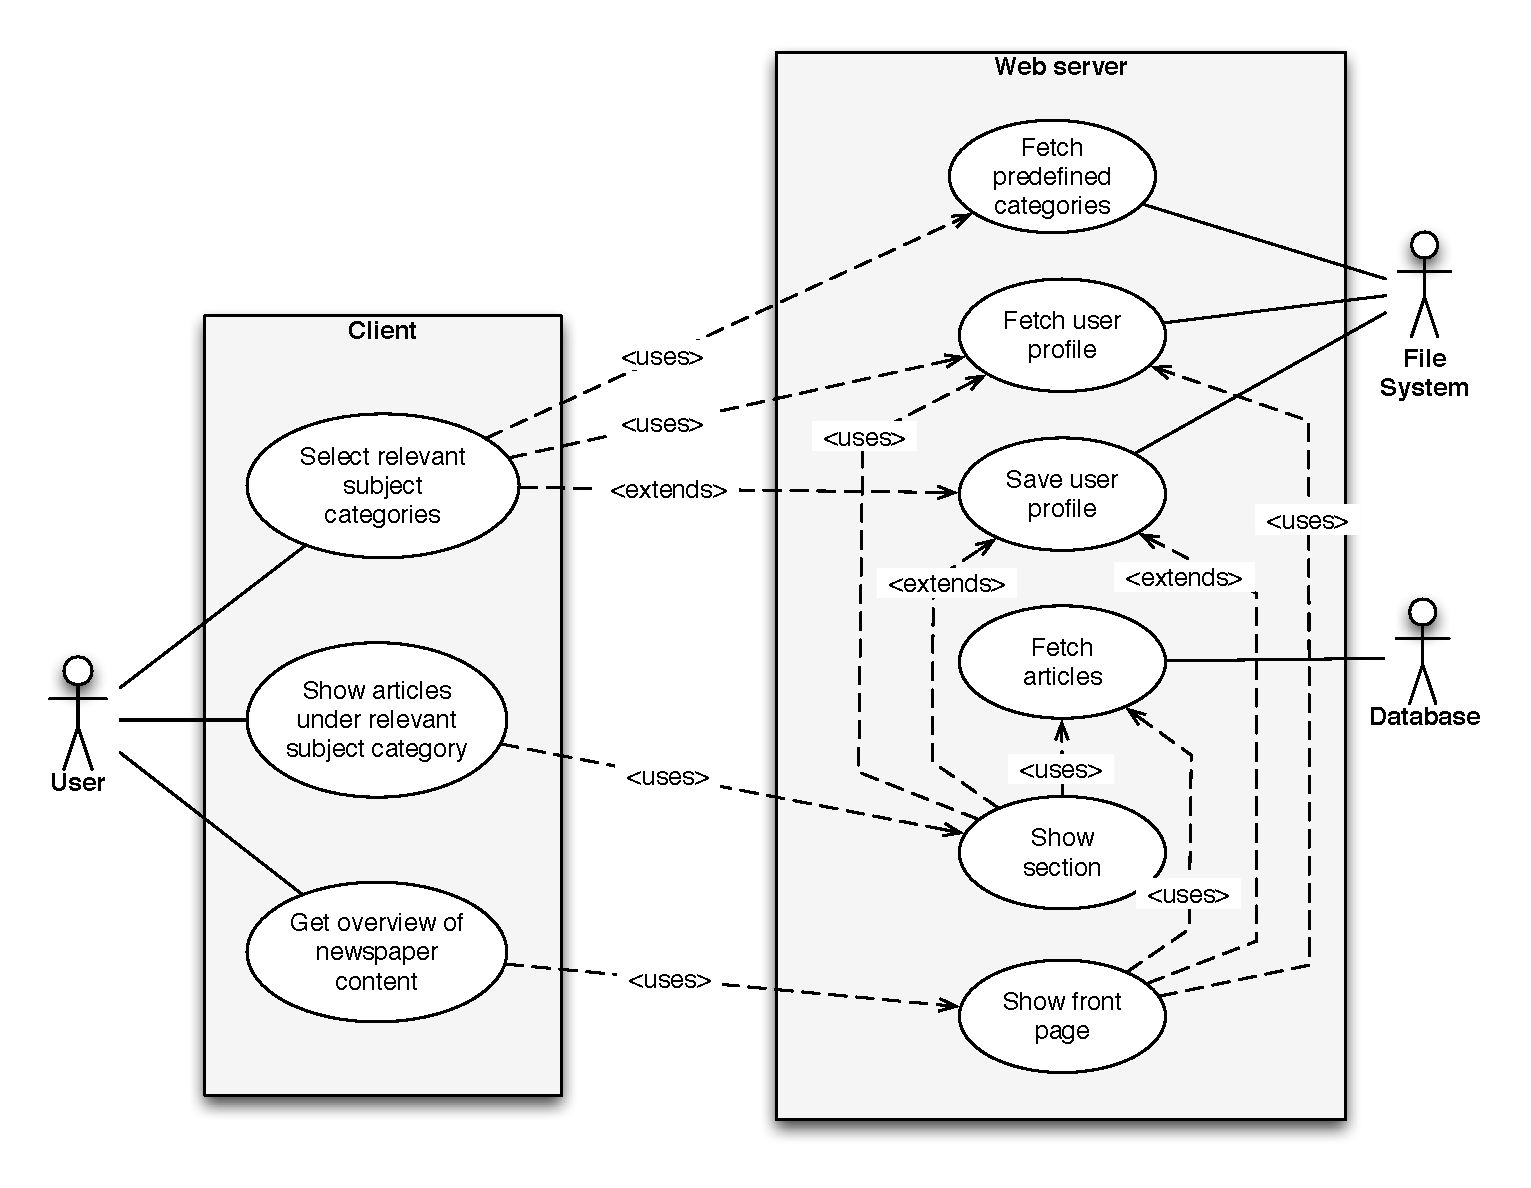
\includegraphics[width=.8\largefigure]{img/use-cases}
	}
	\marginnote{
		\begin{minipage}{\marginparwidth}
			\vspace{-20pt}
			\caption{The figure shows the use cases of the system and how the client side handles them and how the web server acts to accomplish requests from the client side.}
			\label{fig:use-cases}
		\end{minipage}
	}
\end{figure}
In Figure~\ref{fig:use-cases} is shown a use case diagram of how the client side and web server handles use cases. An extra use case has been added in the diagram to show how the system should handle the initial topic selection by the user. The user is able to select relevant topic categories to get an easy start with the application and his choices are thereafter saved to the user profile for later use. The user can thereafter get an overview of the content from the front page or read articles from a selected topic category, both in a nice readable layout and in a composition based on the editorial mix. Moreover, it is possible to get an overview of the articles within a section from a list of headlines from articles contained within it.

From the constraints presented in this section it is possible to derive server tasks. As noted earlier the latter three constraints in equation~\ref{eq:general_unary} could be used as functions to determine if the article is featured or not. It makes sense to do this on the server as a pre-computation along with the similarity and relevance of articles. For this to be possible some metadata on the articles is needed. In order to determine how many columns an article should fill a word count or character count is needed for each article. In addition, it could also be interesting to look at the image sizes, which potentially could hold much information, and in some cases even constitute the body of the article.

The next chapter will present the implementation of the client and server, which constitutes the product of this project.
%
%\todo[inline]{Which design choices to focus on?}
%

% section design (end)
%!TEX root = thesis.tex
\chapter{Implementation} % (fold)
\label{ch:implementation}
This section describes the implementation of the design choices made in the two previous chapters in terms of client side and server side tasks.

The proposed design presented in the previous chapter has accounted for the presented requirements and user needs, but there are some requirements that will not be implemented due to prioritisation.

Chapter~\ref{ch:design1} and \ref{ch:design2} presented an application that accounted for a user model, this chapter will only present how to collect the necessary user data and use it in the application -- and not implement it. It will, however, describe which metadata is needed and how to acquire it.

The social aspects is an important part of the system are also useful channels for awareness. \cite{Tidwell} even states her editorial mix pattern as a social media pattern. Nonetheless, these will not be implemented in the presented application as it does not contribute with new knowledge to the field. The gathered news articles to be used in this project contains both images and videos, but only images will be considered here. It is however trivial to implement support for videos as the same space allocation principles applies, but it was not prioritised.

Also, the personalised summaries have already been very well explored in \cite{fulltext.pdf} and this project will not try to compete with this solution, so only the first few sentences will constitute the excerpts from articles to be used on the front page. Because the full articles are shown in the sections no excerpts will be used in these. This should, however, be supported in the further development of the application.

The sections are based categories. These are by no means complete and they have not been verified. However, they are some of the most recurring in popular news sites and are used in order to proof the concept is possible. Thus, their definitions are not comprehensive either.

Finally, only a subset of the editorial mix constraints, presented in the Constraint Programming chapter (chapter~\ref{ch:design2}), will be implemented. Furthermore, before the user test was done the implementation had already started. This led to the implementation of a fairly complex layout constraint to minimise white space. It turned out that some white space was actually a user preference, but the implementation of the constraint will be presented nonetheless, as it shows a good example of what is possible with the system. 
%
%Whitespace between articles should be minimised. This is not an actual user requirement, but it is included as it a fairly complex layout problem to solve and it shows some aspects of what it can do.
\clearpage
%\section{Server for Acquiring and Mining Data for Personalisation}
\section{Similarity and Relevance {Computation}}
%\subsection{spatial, temporal and relational personalisation}
The \cite{DCMI} proposes 15 metadata elements for documents:
\begin{itemize}\itemdist
	\item Title
	\item Creator
	\item Subject
	\item Description
	\item Publisher
	\item Contributor
	\item Date
	\item Type
	\item Format
	\item Identifier
	\item Source
	\item Language
	\item Relation
	\item Coverage
	\item Rights
\end{itemize}
The articles in this project have been acquired using the Readability API\sidenote{An API to parse articles from websites.} to scrape articles given by links from RSS-feeds. This way it is possible to get the full article. Under normal circumstances, these would probably be supplied by a content provider, say through agreements with newspaper companies or social networks. The Readability API provides several metadata elements for the parsed articles; a domain, a title, an article URL, a lead image, the author, an article excerpt, a word count and a date of publication. This satisfies many of our needs, but there are still some very crucial calculations to be done, i.e.\ the article relevance according to user topics and similarity between articles.

The analysis of article relevance and similarity to other articles will use the same analysis, namely a keyword analysis using the WordNet and entity comparison using the Open Calais API\sidenote{A service by Thomson Reuters that automatically extracts semantic information from web pages in a format that can be used on the semantic web.}. These will be presented in the following.

WordNet is a large lexical database of English words and their relationships in the form of different graphs. WordNet is based on \emph{synsets}, which is a set of synonyms that describes different meanings of the same word. WordNet has a hyperonymy and hyponymy graph for noun synsets, which is based on the ISA relation between words. A \emph{hypernym} relation is a generalisation, e.g.\ a hypernym for a bed is a piece of furniture; and a \emph{hyponym} relation is a specification, e.g.\ a hyponym for a bed is a bunkbed. For nouns there also exists the meronymy graph, which is a graph describing the part-whole relation; a chair e.g.\ has a back, a seat and legs. Also, parts are inherited by superordinates, e.g.\ if a chair has legs, then an armchair has legs as well. Furthermore, WordNet has a graph describing elaboration, i.e.\ \emph{troponyms}, of verbs synsets, adjectives organised in terms of antonymy and adverbs which can be be described in terms of adjectives. The synsets, the hypernym and hyponym graph and the troponym graph of WordNet are the most interesting, because they describe different meaning of a given word, whereas the others describes relation to other words.
%Noun hyperonymy, hyponymy or ISA relation
%Noun Meronymy, inherited
%Verb synsets, troponyms: dimensions along which verbs can be elaborated
%Adjectives are organized in terms of antonymy
%adverbs are straightforwardly derived from adjectives via morphological affixation

The initial approach involved computing the TF-IDF similarity using the Python libraries for this \cite{NLTK}. This approach works on a bow (bag-of-words) with keywords and weights representing a single item. The weight is computed by the number of occurrences in the provided text and a cosine of the angle between them determines the similarity. However, Python also provides an interface for working with WordNet. This allows for a more in-depth analysis of the obtained news articles. \cite{116262780379.pdf} presents an algorithm for enriching articles using WordNet's hypernym graph, which proves to yield precise results in the context of enhancing labelling using K-means clustering. However, only the WordNet enriching of articles will be used to aid the keyword based approach in this implementation. In the presented approach a subgraph of WordNets hypernym graph is generated by the top $20\%$ frequent keywords of an article and weighted by equation~\ref{eq:weight}
\begin{align}
W(d, f) = 2 \cdot \frac{1}{1+e^{-0.125(d^3\frac{f}{TW})}}-0.5
\label{eq:weight}
\end{align}

Where $d$ stands for the node's depth in the graph (starting from root and moving downwards), $f$ is the frequency of appearance of the node to the multiple graph paths and $TW$ is the total number of words used to generate the hypernym graph. An example of such a hypernym graph is seen in Figure~\ref{fig:hypernym-graph}.
\begin{figure}[h!tp]
	\myfloatalign
	%\makebox[\textwidth][l]{
		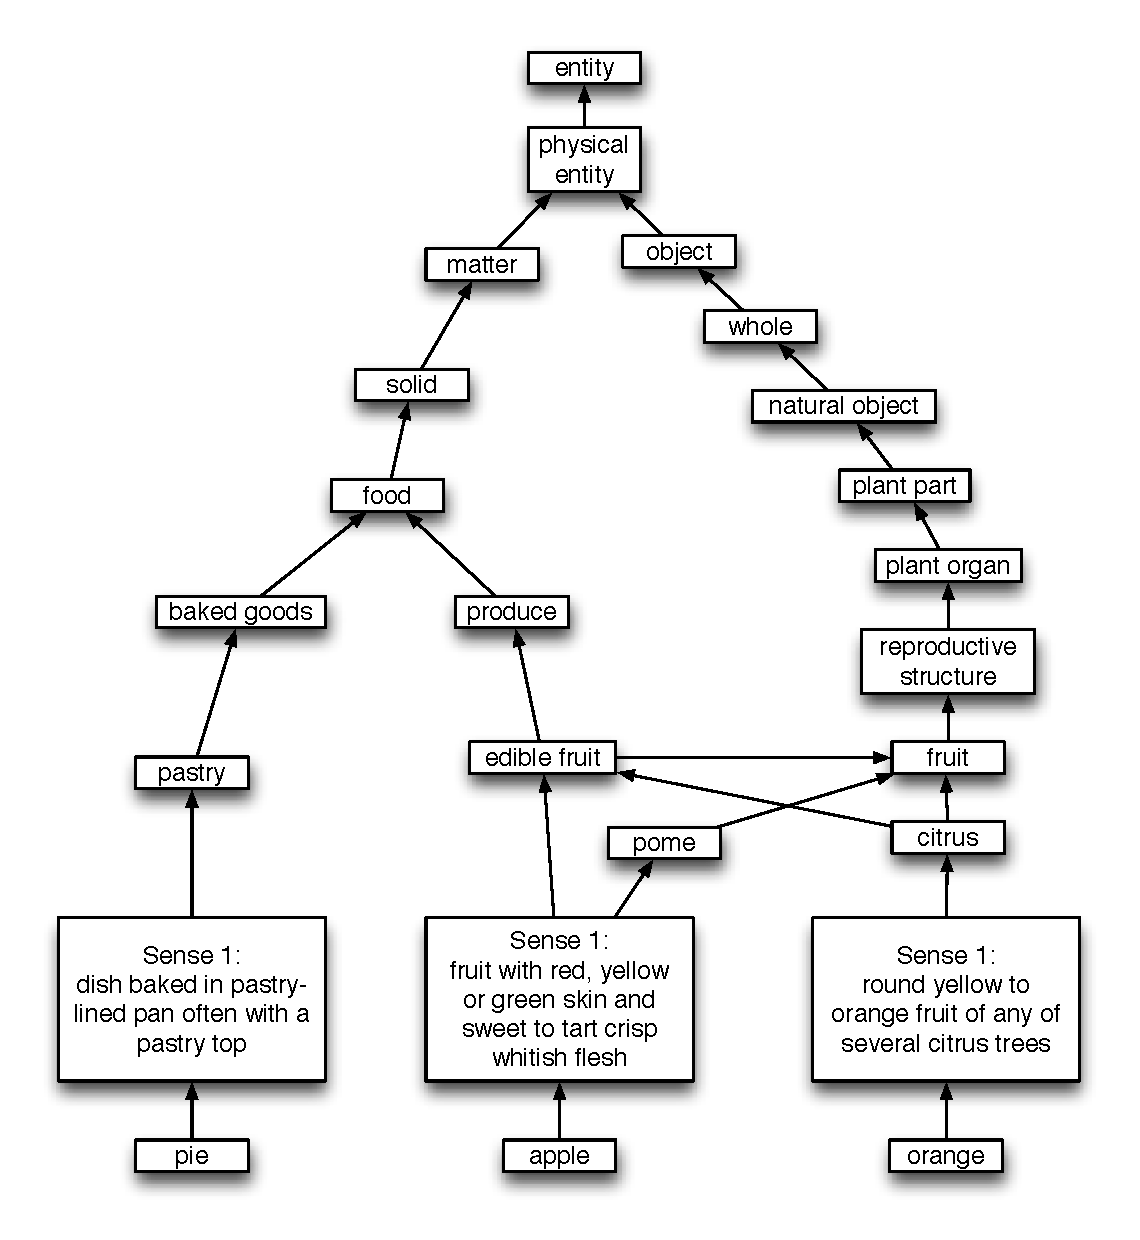
\includegraphics[width=.8\textwidth]{img/hypernym-graph}
	%}
	\marginnote{
		\begin{minipage}{\marginparwidth}
			\vspace{-250pt}
			\caption{The figure shows an example of a hypernym graph that could be generated by the \textsc{WordNet-Enrich}\\ algorithm.}
			\label{fig:hypernym-graph}
		\end{minipage}
	}
\end{figure}

To be able to work with hypernyms, words from articles must be converted to synsets. For each word there exists a synset for each use of the word, with the most frequently used first. Every synset is included in the analysis of this implementation, but in a later stage this could be further focused by only using the top $n$ uses of the word. In the algorithm given by \cite{116262780379.pdf} only the most general use is included (see Figure~\ref{fig:hypernym-graph}), which is a rough assumption. By this it is assumed that the meaning of every word extracted from an article is of the most general use. A better solution would be to use the Wu-Palmer similarity to find the best match of words (\cite{Wu-Palmer}). Wu-Palmer calculates a similarity based on the lowest common ancestor in the hypernym graph, which is available through the Python implementation. This way a set of keywords is gathered based on their most frequently common uses, as opposed to their independently common uses.

WordNet distinguishes among Types (common nouns) and Instances (proper nouns)\sidenote{Common nouns are general words for any people, places and things while proper nouns are specific names of individual people, places, things, or a title.}, so it is possible to extract these from the articles to base the analysis on. Both nouns and adjectives are extracted from articles, but adjectives could also be derived from adverbs to add meaning. A hypernym graph is produced of a maximum of 9 levels up in the graph and each of these synsets are weighted and the top $20\%$ extracted hypernymns along with the top $20\%$ of the original given keywords constitutes the final set of keywords, see Figure~\ref{fig:wordnet_enrich}.
\begin{figure}[ht!p]
	\hspace{-40pt}
	\newsavebox{\wordnetenrichbox}
	\begin{lrbox}{\wordnetenrichbox}
	\begin{minipage}{.75\largefigure}
		\vspace{-5pt}
		\begin{codebox}
\zi \proc{WordNet-Enrich}($a$) \kw{returns} enriched list of keywords
    \Indentmore
\zi \kw{inputs:}
    \Indentmore
    \zi $a$, an article \End
\zi $total\_hypernym\_graph \leftarrow$ a new graph
\zi $kws \leftarrow$ fetch $20\%$ most frequent kws for a
    \zi \For \kw{each} keyword $kw$ in $kws$ \kw{do} \Do
    \zi 	$hgraph \leftarrow$ \proc{WordNet-HypernymGraph($kw$)}
    \zi 	\For \kw{each} hypernym $h$ in $hgraph$ \kw{do} \Do
    \zi			add 1 to frequency of $h$ in $total\_hypernym\_graph$ \End \End
    \zi \For \kw{each} hypernym $h$ in $total\_hypernym\_graph$ \kw{do} \Do
    \zi     $d \leftarrow$ calculate depth of $h$ in WordNet hypernym graph
    \zi     $f \leftarrow$ frequency of $h$
    \zi     $weight \leftarrow 2 \cdot \frac{1}{1+e^{-0.125(d^3\frac{f}{\proc{size($kws$)}})}}-0.5$ \End
    \zi \proc{sort-weights($total\_hypernym\_graph$)}
    \zi $important\_hypernyms \leftarrow$ top $\frac{\proc{size($kws$)}}{5}$ of $total\_hypen\_graph$
    \zi \Return $kws \leftarrow kws + important\_hypernyms$
    \End
		\end{codebox}
		\vspace{-5pt}
	\end{minipage}
	\end{lrbox}\fbox{\usebox{\wordnetenrichbox}}
	%\marginnote{
	%	\begin{minipage}{\marginparwidth}
			\caption{The \proc{WordNet-Enrich} algorithm for enriching articles using hypernym graphs from WordNet, inspired by~\protect\cite{116262780379.pdf}.}
			\label{fig:wordnet_enrich}
	%	\end{minipage}
	%}
\end{figure}

After this extraction the similarity is computed by a path similarity, which is based on the shortest path between the words, on the best matches between words. The Wu-Palmer similarity, could again, be used instead, but to avoid more computation time the naïve solution was chosen.

Because it is possible to distinguish between proper nouns and common nouns in WordNet as well, this was used to extract instances from articles. However, WordNet often seemed to have problems with this particular issue and would, e.g.\ match an article about an exhibition of Claude Monet's flower garden to a topic containing the company Apple inc.
\begin{figure}[h!tp]
	\myfloatalign
	\subfloat{\includegraphics[width=.5\largefigure]{img/monet-small}}%
	\\
	\subfloat{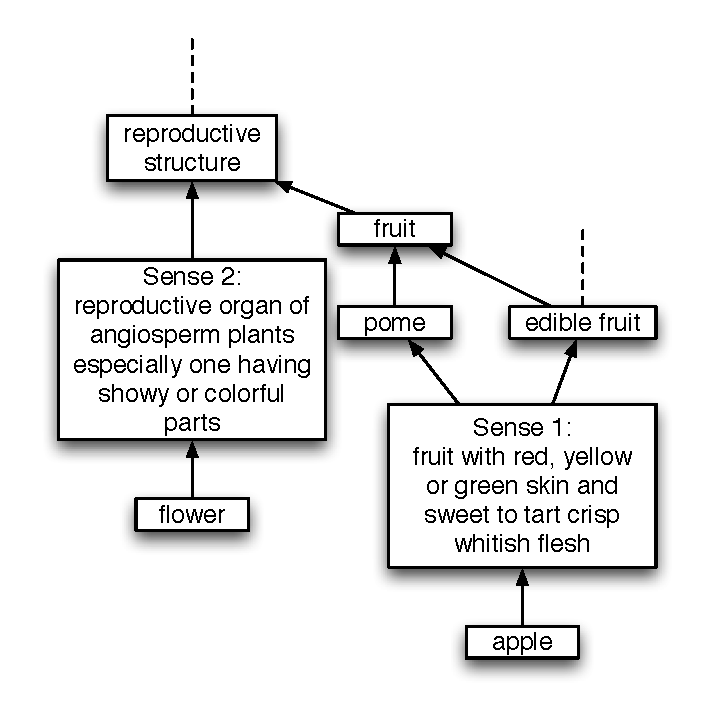
\includegraphics[width=.5\largefigure]{img/flower-apple}}%
	%\makebox[\textwidth][l]{
		%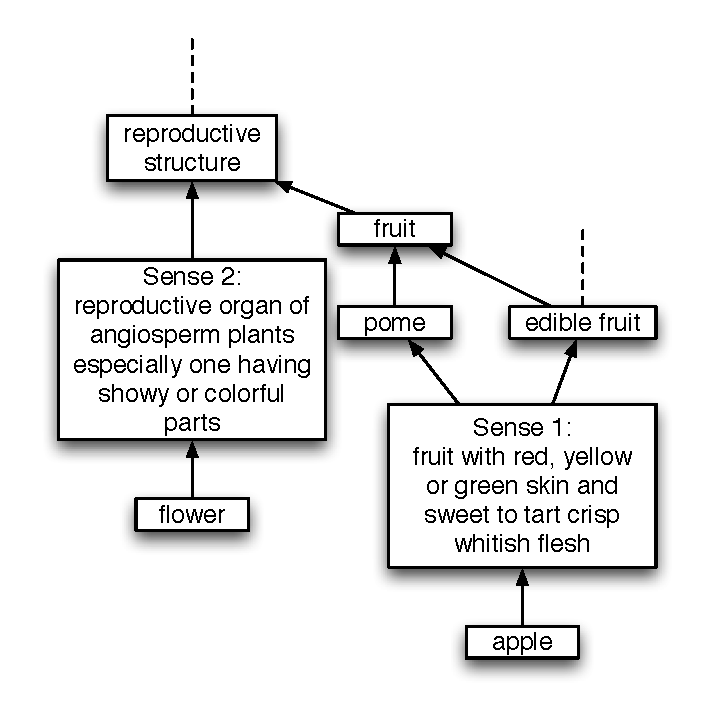
\includegraphics[width=.5\textwidth]{img/flower-apple}
	%}
	\marginnote{
		\begin{minipage}{\marginparwidth}
			\vspace{-370pt}
			\caption{The figure shows an example a close realtion in the hypernym graph of the words ``apple'' and ``flower''.}
			\label{fig:flower-apple}
		\end{minipage}
	}
\end{figure}

An example of where Wordnet does not perform well is New York. When the words are removed from each other, they provide another meaning, which is what the implementation supply WordNet with. But Open Calais can handle the full document and can detect where to keep the words together in order to find meaning.

To account for this a similarity using the Open Calais API was implemented.
%\todo[inline]{WordNet distinguishes among Types (common nouns) and Instances (specific persons, countries and geographic entities). (\url{http://wordnet.princeton.edu/})}
%\todo[inline]{level is only a part Python implementation of WordNet}

The Open Calais API provides analysis of documents and extraction of several kinds of metadata. This implementation will only use the extraction of entities, but it could however, be interesting to see how well the document categorisation performs, which includes many general news topics. After the extraction of entities the similarity is calculated by the sum of entity matches divided by the average length of the two given entity sets.

The final similarity is found by the average of the WordNet similarity and the entity similarity. This seemed to form a solid structure for computing the similarities between articles, but the relevance according to the user defined topics needs to be calculated as well. Fortunately, the decision of using keyword based user models lets us use the same functions to compute similarity between articles and topics. In Figure~\ref{fig:simplot} is a plot of similarities between articles and 9 different topics. The similarities are ordered by an average between them.
\begin{figure}[h!tp]
	\myfloatalign
	\makebox[\textwidth][l]{
		\includegraphics[width=.88\largefigure]{img/simplot}
	}
	\marginnote{
		\begin{minipage}{\marginparwidth}
		\vspace{-120pt}
			\caption{The figure shows a plot of articles with WordNet and Open Calais similarities, their average and a plot of the standardised average.}
			\label{fig:simplot}
		\end{minipage}
	}
\end{figure}

These similarities between articles, worked well but was somewhat strict. The highest similarity given was $0.396$ in a range of $[0;1]$. $86\%$ of them was below $0.1$. Because of this and that even fairly low similarities yielded promising results it seemed appropriate to standardise it. This is also plotted in Figure~\ref{fig:simplot}. The standardising of the data is done by taking the logarithmic function of their percentages to flatten it more and dividing it by the largest similarity to spread it evenly over the $[0;1]$ scale.

The articles are stored in a file on the server for easy retrieval by the client side and the metadata is stored in a database. The articles could have been stored in a database along with the metadata for a more sustainable solution, but this was just an easy solution.
%\subsection{Computing Similarity}
%- Storing Data

%\section{Client for Composing the Editorial Mix and Presenting the Articles}
\section{Interface}
In order to fulfil the requirements of a column based interface it seemed appropriate to use a grid based layout. Twitter Bootstrap\sidenote{A collection of tools for creating web applications.} provides an excellent framework for this which is both touch friendly and responsive\sidenote{Responsive Web Design means that the layout is adaptable to the viewing devices screen size.}. A layout was developed using conditional styling so an article can be assigned a class according to its size in columns so the layout can adapt to display the article differently according to size. An article that uses 3 columns in landscape mode should necessarily only uses the available 2 columns in portrait mode. This also promotes the possibility of having articles that displays in 1 column in portrait and 2 columns in landscape and finally articles that display 1 column in both.

The calculation of how many columns an article should use was done as a preprocessing, first by the largest image found along with the article and next the number of characters in the article. Users from the test pointed out that images should be as large as possible, and this should therefore dictate the space allocated for the article.

There are different ways of displaying text in columns on the web, but one of the newcomers is CSS3 Multi Columns\sidenote{See \url{http://www. w3schools.com/css3/css3_multiple_columns.asp}.}, which introduces easy styling of text in balanced columns. It was chosen to use this technology to see what was possible with it and because it is a technology that is under development. This means that it is not possible at the moment to divide the columns or let, e.g.\ an image span a number of columns using styling. Either an object has to span all columns or be wrapped into one, but their respective functionality is however soon to be supported. One could manually implement the division of columns, but it was deemed unimportant for the project to investigate this further. This means that some white space beside images might occur and that columns continues with no division.
%\todo[inline]{css: conditional styling}

The main page of the application is created dynamically. User preferences are registered from the from submission and saved locally. If the view changes, the articles from the former section is removed and the new ones are inserted in their place. This provides the possibility of introducing animations between section changes and lazy load of the pages.

In Figure~\ref{fig:sequence} is shown a sequence diagram of what the system does in order to display the front page (or a section), when the user opens the application.
%\sidecaptionfigure{\textwidth}{img/sequence}{The figure shows a sequence diagram from when the user chooses a topic category until he can read articles from this topic. \texttt{secNum} is the section number to display (the front page is section 0), \texttt{userId} is a string that identifies the user, \texttt{userPrefs} is the user preferences on the specific section and \texttt{articles} is the library of articles to compose the editorial mix of.}{fig:sequence}
%\begin{figure}[h!tp]
%	\myfloatalign
%	\makebox[\textwidth][l]{
%		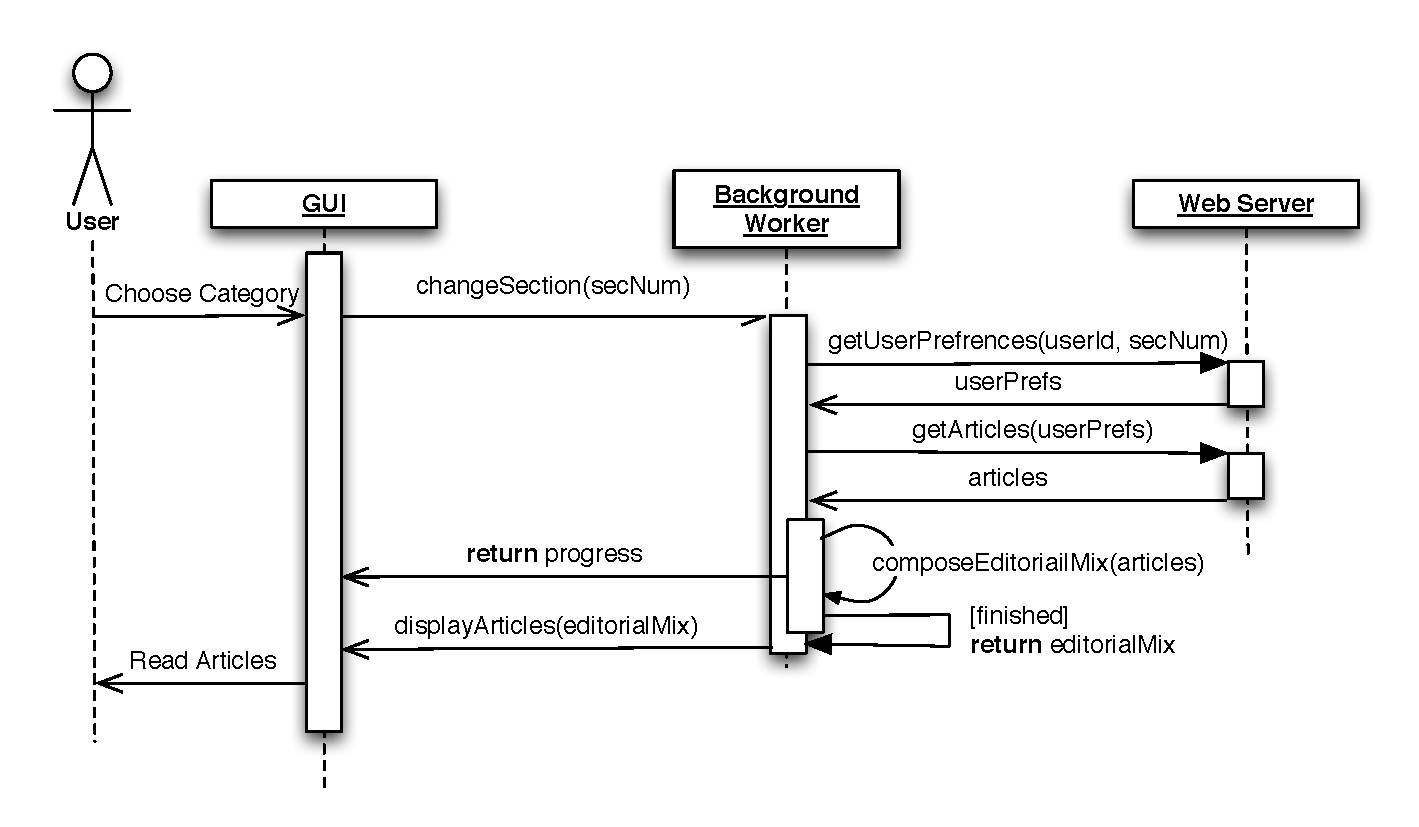
\includegraphics[width=.8\largefigure]{img/sequence}
%	}
%	\marginnote{
%	\vspace{-50pt}
%	\begin{minipage}{\marginparwidth}
%		\caption{A sequence diagram from when the user chooses a topic category until reading articles. \texttt{secNum} is a section number, (front page is section $0$), \texttt{userId} the user id, \texttt{%userPrefs} the user preferences on a given section and \texttt{articles} is a library of articles to compose the editorial mix of.}
%	\label{fig:sequence}
%		\end{minipage}
%	}
%\end{figure}
\begin{figure}[h!tp]
	\centering
	
	\def\mygraphic{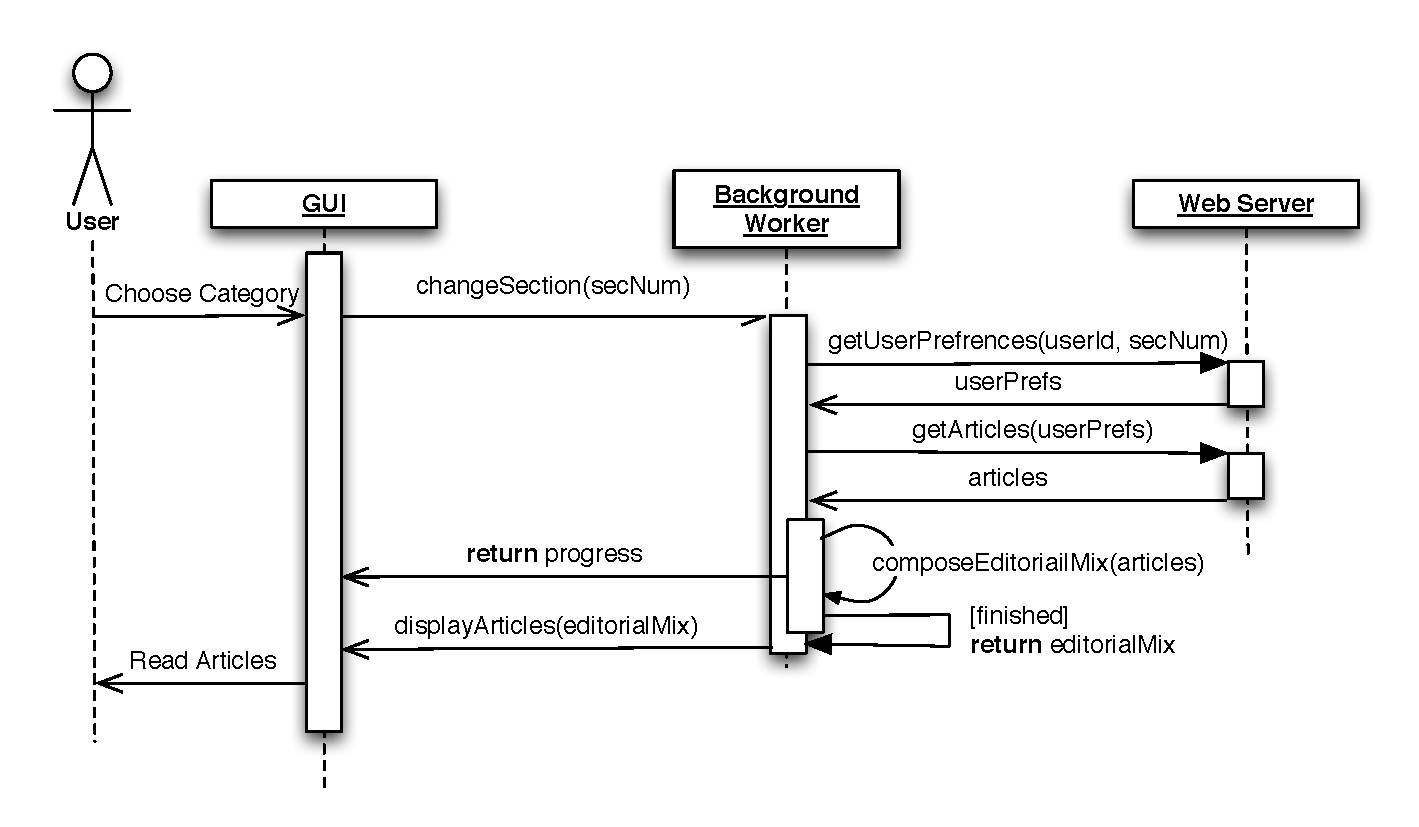
\includegraphics[width=\textwidth]{img/sequence}}
	%\newlength{\graphicheight}
	\settoheight\graphicheight{\mygraphic}
	\mygraphic
	\marginnote{
	\begin{minipage}{\marginparwidth}
		\vspace{-\graphicheight}%
		\caption{A sequence diagram from when the user chooses a topic until reading articles. $secNum$ is a section number, (front page is section $0$), $userId$ the user id, $userPrefs$ the user preferences on a given section and $articles$ is a library of articles used to compose the editorial mix.}
		\label{fig:sequence}
		\vspace{\graphicheight}
		\end{minipage}
	}
\end{figure}
%\begin{figure}[h!tp]
%	\myfloatalign
%		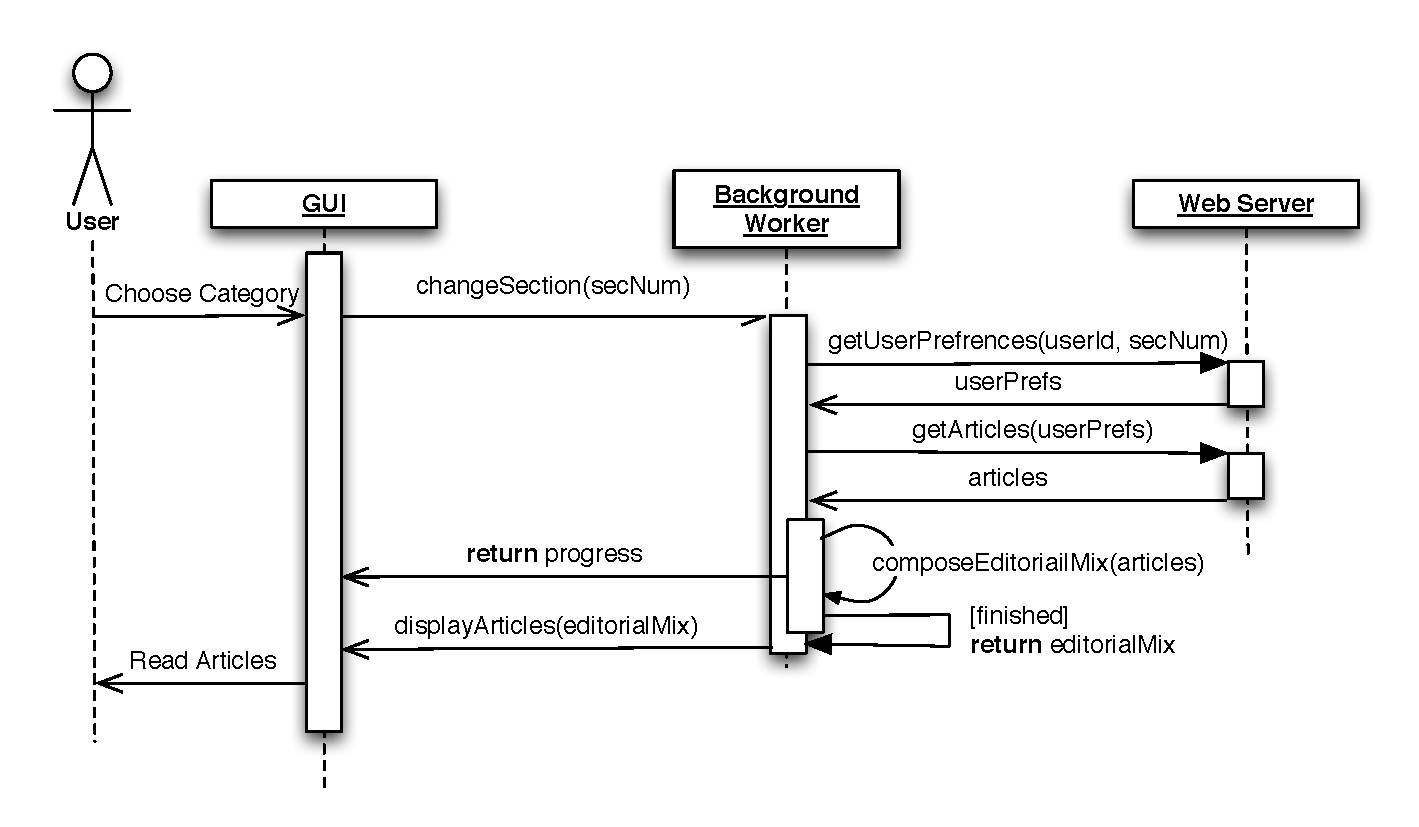
\includegraphics[width=\textwidth]{img/sequence}
%	\caption{The figure shows a sequence diagram from when the user chooses a topic category until he can read articles from this topic. \texttt{secNum} is the section number to display (the front page is section 0), \texttt{userId} is a string that identifies the user, \texttt{userPrefs} is the user preferences on the specific section and \texttt{articles} is the library of articles to compose the editorial mix of.}
%	\label{fig:sequence}
%\end{figure}

When the application is opened, or the application is changed to display a section, a background worker is initialised to compose a mix of articles. If the mix of articles in a section, or the front page, have already been computed, it should not have to recompute it. The background worker needs to get both the user preferences of the chosen topic and articles that potentially fit the user preferences. While the worker computes the editorial mix it sends messages to the user interface about the progress. This is used to provide feedback to the user. When it finishes the user interface is asked to display the articles.

The implementation does not log user behaviour and does not support relevance feedback to be stored in a user model. The user model have been manually written with manual definitions of keywords and their respective weights for sections. It was chosen not to focus on the logging of data to represent the user model, because it does not contribute with new knowledge to the field. The logging of data could, however, be done by detecting when an article enters the screen, e.g.\ using jQuery Waypoints\sidenote{A small jQuery plugin that makes it easy to execute a function whenever you scroll to an element.}. jQuery Waypoints provides events whenever an item enters the screen, then a time stamp could be registered and stored with a duration, when a new article enters the screen. Problems might, though, emerge when more articles are shown on the screen at the same time. Which article does the user read? A solution to this could be to register the touch, as the user might interact more with the screen in some places based on the position of the article he reads. This project will leave the problem to its field of study.
%\todo[inline]{Noget om hvordan programmet kunne samle keywords med vægte for en bruger?}

The next section will describe how the background worker handles its assigned tasks.

\section{Background Worker}
The choice of using a background worker to do the computation is essentially based on minimising the work for the UI thread. Web Worker\sidenote{A JavaScript script that runs in the background, independently of other, user-interface scripts that may also have been executed from the same HTML page.} introduces long-running JavaScript scripts which are not interrupted by scripts that respond user interactions, and allows long tasks to be executed without yielding to keep the page responsive. With this supporting browsers assigns a thread to handle the background worker tasks, but it remains in the same process.

Background workers are not meant to be numerous, because they require a high start-up performance cost and per-instance memory cost. On this basis a background worker was build to handle the section constraints and the front page constraints, respectively. In the further development it would make more sense to merge the two files, as they share a lot of code. It did however give a nice division between their respective assignments. When the user has submitted the form, as described in section~\vref{sec:layout_typography}, a background worker is asked to compute the editorial mix. It first creates the COP, with variables based on the user input, their respective domains and constraints to fit the section. Information is sent from the main script to the worker, so it can base the constraints on this, e.g.\ a list of articles from the front page is sent when a section should be composed. This way the knowledge is kept in the main script and shared amongst workers to be applied in specific problems. After the COP has been created it fetches potential articles and calls a library to do the constraint computation.

\section{Constraint Personalisation Library}
A library was developed for solving personalisation problems using CP. It was implemented using the \textsc{Min-Conflicts} algorithm along with the MCV heuristic to guide the selection of variables. The motivation for building the library comes from a need of a CP library that supports the use of a list of values consisting of real world items instead of having to define the items as a sub-problem. This section will describe how to use it and discusses the choices of implementation. The library is from here on referred to as \emph{Constraint Personalisation Library} or CPL\sidenote{The library can be downloaded here: \url{http://lestrade.imm.dtu.dk/~s062596/js/cp.js}.}.%the data structure, its general purpose solver

The library provides the possibility for creating a list of variables, with their respective domains and subdomains, see Table~\ref{code:domain}.
\begin{table}[h!tp]
\caption{Declaration of a domain, subdomain and variable}\label{code:domain}
\begin{lstlisting}{JavaScript}
var d = new Domain();
d.addSubdomain(
	// descrete domain (min, max, gap)
	new Subdomain(0, 1, 1),
	// subdomain name
	'images',
	// function for retrieving value attr
	function(x) {
		return x.images.length >= 1? 1: 0;
	}
);
// variable at position 0
var variable = new Variable(0,d);
cop.variables.push(variable);
\end{lstlisting}
\end{table}

After variables and domains have been declared it is possible to declare constraints on them, see Table~\ref{code:constraint}.
\begin{table}[h!tp]
\caption{Declaration of a constraint}\label{code:constraint}
\begin{lstlisting}{JavaScript}
var c = new Constraint(
	// constraint name
	'image0',
	// violation function
	function(vars) {
		if (vars[0] > 0) { return 0; }
		return 1;
	},
	// name of subdomain to work on
	'images',
	// variable positions to get
	// in the violation function
	[0]
);
cop.constraints.push([[c]]);
\end{lstlisting}
\end{table}

The constraints of the COP is stored in a list of lists of lists for two reasons. Firstly the nested list of nested lists is interpreted as a conjunction of disjunctions of conjunctions. The outermost conjunction is interpreted as the set of constraints, where the inner disjunction of conjunctions is interpreted as a decomposition of the constraint. This is to make it possible for the developer to declare a list of alternate sub-constraints as a decomposition of a constraint, i.e.\ it is possible for the user to declare a set of sub-constraints where either one of them should be fulfilled in order to satisfy the rule. This means that $[[[c_1,c_2],[c_3]],[[c_4]]]$ would be interpreted as $((c_1 \wedge c_2) \vee c_3) \wedge c_4$, where $c_1$ to $c_4$ are constraints.

An example of where this can be used is in the earlier described \texttt{image} constraint (see equation~\vref{eq:section_constraints}). This constraint is defined on 4 variables, where either one of them should have an image for the constraint to be fulfilled. Instead this could be described as a list of four lists with one constraint in each. Constraints that each looks like the one presented in the Table~\ref{code:constraint}, on variables in position 1 to 4, 4 to 7, 7 to 10, etc. There might also emerge situations where it could be useful to have alternating conjunctions of constraints. An example of this is the earlier mentioned white space minimisation, which is expressed as a more complex constraint.

The minimisation of white space can be expressed in terms of columns as; the accumulated sum of the columns assigned to articles in the problem in the next step minus the accumulated sum in the former step always be dividable with both 2 and 3. The following boolean expression expresses the same:
\begin{align*}
	&(sum_i-sum_{i-1} < 2 \vee sum_i-sum_{i-1}\ \texttt{\textbf{mod}}\ 2\ \neq 0) \wedge\\
	&(sum_i-sum_{i-1} < 3 \vee sum_i-sum_{i-1}\ \texttt{\textbf{mod}}\ 3\ \neq 0)
\end{align*}
Where \texttt{\textbf{mod}} is the modulus function.

In other words; any composition of articles should always fill out the screen in both portrait and landscape. Many possibilities for achieving this is available. For a list of three articles, this could be done by having three articles where each would have $2.5$ columns assigned. An article that is assigned $2.5$ columns means that is fills two columns in portrait and three in landscape, whereas an article assigned $1.5$ would display in one column in portrait and two in landscape. A more complex function could also describe the possibilities for two articles in a row, or three, or even more. The constraints could therefore be described as a disjunction of conjunctions as the following:
\begin{equation}
\begin{split}
[&[columns_0, columns_1, columns_2],\\
&[columns_{0-1}, columns_2],\\
&[columns_{0-2}]]
\end{split}
\label{eq:col-row}
\end{equation}
\begin{equation}
\begin{split}
((&columns_0 \wedge columns_1 \wedge columns_2) \vee\\
(&columns_{0-1} \wedge columns_2) \vee\\
&columns_{0-2})
\end{split}
\label{eq:col-row-logic}
\end{equation}
Where the number denotes which variable positions in the problem the constraint works on. A declaration of a white space minimising constraint over two variables is seen in Table~\ref{code:cols-constraint}.
\clearpage
\begin{table}[h!tp]
\caption{Declaration of a constraint for minimising white space}\label{code:cols-constraint}
\begin{lstlisting}{JavaScript}
var c = new Constraint('columns0-1',
	function(vars) {
		var violation = 0;
		if (vars[0] == 1) {
			if (vars[1] != 1.5) {
				violation++;
			}
		} else if (vars[0] == 1.5) {
			if (vars[1] != 1) {
				violation++;
			}
		} else {
			violation++;
			if (vars[1] != 1 && vars[1] != 1.5) {
				violation++;
			}
		}
		return violation;
	}, 'columns', [0,1]);
cop.constraints.push(c);
\end{lstlisting}
\end{table}

The second reason for this representation of constraints is that it is possible to declare constraints on fewer variable and that it is possible for the system to prune some calculations. The first constraint in a disjunction that evaluates to true, or in this case to violation $0$, makes it possible to discard the rest of the constraints in that disjunction. If the constraints are then ordered by how many variables they work on, so the system tries to evaluate the constraints in a conjunction that is defined on fewest values first, then it may never have to evaluate constraints that are global. In worst case it would have to evaluate all of them. An example of this ordering is seen in equation~\ref{eq:col-row} or \ref{eq:col-row-logic}, where the first nested list is only of unary constraints, the second a list of a binary and an unary and finally a single global constraint. However, it is also worth deciding how important it is that the application explores more complex solutions if simpler solutions works just as well. In any case it leaves the possibilities for the developer to optimise his definition of the problem. In further development it could be interesting to explore automatic reduction and organisation of constraints.

\cite{AIRussell} proposes constraint weighing to aid the organisation and furthermore maybe even lead the search to concentrate on variables that is bound by these constraints to solve them first. Constraints in this implementation are only represented as preference constraints, so every constraint returns a violation. This aids the search towards concentrating on changing variables that yields a lesser violation, but it also means that the returned assignment could violate constraints that are not supposed to be violated if the algorithm had trouble with finding a solution for the given problem. Using solely preference constraints eliminates the possibility of letting the search go on until a solution has been found. On the other hand one could argue, with a fixed budget computation problem, it is better to deliver the best assignment so far, than nothing at all.
%\subsection{Data Structure}
%\subsection{General Purpose Solver}
%Preference ordering of hard constraints or division between preference constraints and hard constraints.
%Assignment from library instead of arbitrary assignment? The latter is a more hypothetical approach. Providing the library as a constraint, where each variable assignment must have a unique combination from one of the possibilities of the constraint.
%(sim,breaking,chars,date,sections?,columns):list
%The former introduces an implicit constraint in that the general purpose solver can only choose from the library, thus can only choose a combination of values that exists.
%
%\todo[inline]{Ranges can be optimised in space by converting them to integer ranges. This can be done by setting min = 0 and max = (b-a)/gap.}
%The library could take any combination of constraints and then organise them into conjunctions of disjunctions, with the constraints taking fewer values first.
%In the implementation this is done by hand, so the program takes conjunctions of disjunctions of constraints organised with constraints that takes fewer values first. Constraint weighing could also help organising the disjunctions and furthermore lead the search to concentrate on variables that is bound by these constraints. (p. 222 AIRussel).
%
%\todo[inline]{Constraints should point to specific variables, this makes it somewhat rigid/ineffective because I have to write at global constraint that accounts for everything (ineffective in propagation -- might also be a problem if it does not show progress in changing values, i.e.\ it is a hard constraints and not returning a cost of the set of values.) or divide it into smaller constraints separated by an `or' (v). The latter is ineffective because there would should be a combination of constraints accounting for every situation, e.g. if the first variable is satisfying an unary constraint, the next say 3 variables (if the problem holds 4 variables) could satisfy three unary constraints, an unary and a binary (two combinations exists) or a constraint that takes three variables. This grows fast with the number of constraints.}
%
%\todo[inline]{Does it make sense that a continuous range cannot have specific values removed? Should it be possible for it be divided into subranges if the user decides to remove a range of values in between its domain of [min;max]?}

Constraints that have been implemented to compose the sections are \texttt{all-diff}, \texttt{fp-articles}, \texttt{topic}, \texttt{main-stories}, \texttt{adj-subj}, \texttt{images} and constraints to minimise white space. Also, the \texttt{featured-image} and \texttt{nonfeatured-image} have been implemented, but only as the same constraint that prefers images on every article, meaning that there is not a distinction between featured and non-featured articles.

Screenshots of the final implementation is seen in Figure~\ref{fig:screenshots} and can be accessed on \url{http://lestrade.imm.dtu.dk/~s062596}.

\begin{figure}%
%\centering%
\makebox[\textwidth][r]{% %%% as above; this time, the
%%% figures flushes from the left
\subfloat[Screenshot of the form.\label{fig:screenshot1}]%
	{\includegraphics[width=.33\largefigure]{img/screenshot1}}%
	\qquad%
\subfloat[Screenshot from the sports section.\label{fig:screenshot2}]%
	{\includegraphics[width=.43\largefigure]{img/screenshot2}}%
}
\\
\makebox[\textwidth][r]{% %%% as above; this time, the
\subfloat[Screenshot from the technology section (portrait).\label{fig:screenshot3}]%
	{\includegraphics[width=.33\largefigure]{img/screenshot3}}%
	\qquad%
\subfloat[Screenshot from the technology section (landscape).\label{fig:screenshot4}]%
	{\includegraphics[width=.43\largefigure]{img/screenshot4}}%
}
\caption{The figure shows four screenshots of the final implementation.}%
\label{fig:screenshots}%
\end{figure}

The next chapter will evaluate the solution in terms of quality and performance.

% section design (end)

\cleardoublepage % Empty page before the start of the next part

%------------------------------------------------
\addtocontents{toc}{\protect\newpage}
\ctparttext{Evaluation of the solution and discussion of uses in new contexts.} % Text on the Part 1 page describing  the content in Part 1
\part{Evaluation and Perspectives}

%!TEX root = thesis.tex
\chapter{Evaluation} % (fold)
\label{ch:evaluation}
%- Evaluate the solution and compare existing techniques for personalisation to the ones used in the solution.
This section evaluates the implementation as a solution to the problem of personalising the editorial mix and Constraint Programming as a technology for creating personalised web applications.
%
%\todo[inline]{What things were even better or a little worse than expected regarding the methods you used to solve your problems. How could your project be improved by further work.}

%\subsection{Result}
\section{Test}
The test described in Table~\vref{tab:test-description} was conducted on 7 test persons. This is not a solid ground to base decisions upon, but it has been helpful in finding some tentative problems. Main design choices should, in the further development of this application, be verified on a larger empirical basis.

The editorial mix has been conducted on rules inferred from analysis of conventional newspapers. It has not been verified that the composition of articles using these rules actually satisfies user needs better in a digital environment -- even if users are unaware of them. This could be done by turning constraints on and off in the system and presenting them to users, so they can give their feedback on the best composition. In addition, new rules could be added to test new hypotheses. It could for example be interesting to explore users' preferences on the two rejected reading behaviours presented in \cite{holsanova2006entry}:
\begin{itemize}\itemdist
	\item Readers Prefer new information and expect this to be on the right in the semiotic space
	\item Readers scan the semiotic space before taking a closer look at certain units
\end{itemize}

The next section will evaluate the interface of the application.
%\todo[inline]{NOT ONLY 5 test persons \protect\cite{NielsenTest}. This has been discarded by many.}
%\cite{NielsenTest} says that 5 test persons in a qualitative test is enough to uncover most preferences and issues, but the test included 7 test persons to be more adequate.
%
%\todo[inline]{Hvor langt tid er en artikel interessant > hvor lang tid er en annonce interessant.}

\section{Interface}
In the implemented layout no visual difference between featured articles was supplied. Articles was just supplied with more space if the contents could fill it out. In the further development of the application a distinction between featured and non-featured content should be applied as described in the presented constraints in section~\vref{sec:problem_representation}. This way content distinction can be applied visually.
%\todo[inline]{Implement visual difference between featured articles and non-featured articles.}
%classify items as first and second articles and use layout to distinguish them.

The implemented columns constraints does not always provide good solutions, because they account only for horizontal features of the articles and not vertical. Therefore problems emerge when long-length articles are placed beside short-length articles leaving a lot of white space under the short. The implementation of this fairly complex constraint show that it is possible to implement constraints layout, but that it is hard to formalise and account for every detail. Therefore it worthwhile extracting key features about the layout that is needed to be handled and spend time on reducing constraints to a minimum, let other technologies handle these problems or explore a combination. A constraint that would co-operate with the positioning of articles using jQuery Masonry\sidenote{A layout plugin for jQuery, that arranges elements vertically then horizontally according to a grid.} could be a solution for this. Here it is worth noting that the automatic placement could destroy the combinatorial work of the constraints. However, it seems that jQuery Masonry works to keep the chronological structure of elements, which minimises the harm it can do.
%We follow a strict vertical structure, but there is a lot of work to be done with the horizontal structure

At an early stage, the pagination on a section was discarded, because a preliminary test (ask around) showed that users wanted to scroll down to see the full section. This was also necessary if full-length articles were to be shown, but the reading behaviour analysis suggests that articles should be divided into chunks of subjects, which may be better to visualise using pages. Following the reading behaviours more strictly, the featured article could be shown with large headlines, large images and a longer length excerpt, and stories on the same subject could surround it with only headlines, smaller images and short excerpts. If the user then wants to read one of the articles in full length, he can select it, and the article could be displayed in full, using the whole screen.%Non-featured article he could select it, showing interest in it, and the system could generate a new page where this article is featured. The article should then again be surrounded by new non-featured articles, that of course are not placed anywhere else in the paper.
%
%\todo[inline]{Archive functionality}
%\todo[inline]{Text can be read out loud}
%\todo[inline]{Find more images online}
%\todo[inline]{Negative keywords, using WordNets antonym graph}
%\todo[inline]{Breaking alert, tags på artikler}
%\todo[inline]{har jeg skrevet om at slå constraints fra eller til for at teste?}

Furthermore, \cite{kristin-fredrik.pdf} suggested ads in the application, but it was implemented. It is, however, possible specific to extract keywords and weights for a user on a topic basis. This could be done by direct relevance feedback from the user and by implicit relevance feedback by how long time a user spends on an article, as described in the former chapter. The new weights on keywords can be assigned based on the user behaviour in combination with the calculated weight from the article. This is actually in line with what Google AdSense\sidenote{A program that allows publishers of content sites to serve targeted adverts to site content and audience.} does. AdSense is build on analysing the semantic structure of documents using WordNet, but might include other techniques (\cite{Oingo1} and \cite{Oingo2}).
%\todo[inline]{Give dem de mest optimale ord hele tiden, ville jeg kunne optimere Googles valg af reklamer. Facebook skal key word analysere for at kunne skabe værdi.}
%\todo[inline]{Trending (Google trending): hvad er in for tiden? bruge det til at holde reklamer up-to-date. AdWords eller AdSense?}

The application is implemented with a responsive design, with a layout that is familiar to that of a conventional newspaper. It has explored some possibilities for having full articles in balanced columns with a flat navigational structure of user defined topics.

\section{Content}
This section will analyse and discuss the solution with regards to content.

Similarities were computed with respect to manually defined topics\sidenote{The definitions can be seen in Table~\ref{tab:topic-specification1} and \vref{tab:topic-specification2}.} and with respect to articles in between. To test whether similarities actually make sense it seems logical to look at similarities of articles that match a topic and articles that do not match. The feeds of the gathered articles are often categorised under a certain topic. These topics were saved as tags on each of the articles, and it was then possible to analyse the similarities of articles that hold tags that match the defined topic and which do not. Figure~\ref{fig:sim-analysis} shows averages and minimum and maximum of similarities distributed on the defined topics on articles that hold a tag matching a topic and articles that do not hold a tag matching the topic, respectively.
\begin{figure}[h!tp]
	\myfloatalign
	\subfloat[Similarities of articles that matches the section.\label{fig:sim-match}]{\includegraphics[width=.8\textwidth]{img/sim-max}}%
	\\
	\subfloat[Similarities of articles that do not matches the section.\label{fig:sim-mismatch}]{\includegraphics[width=.8\textwidth]{img/sim-min}}%
	%\makebox[\textwidth][l]{
		%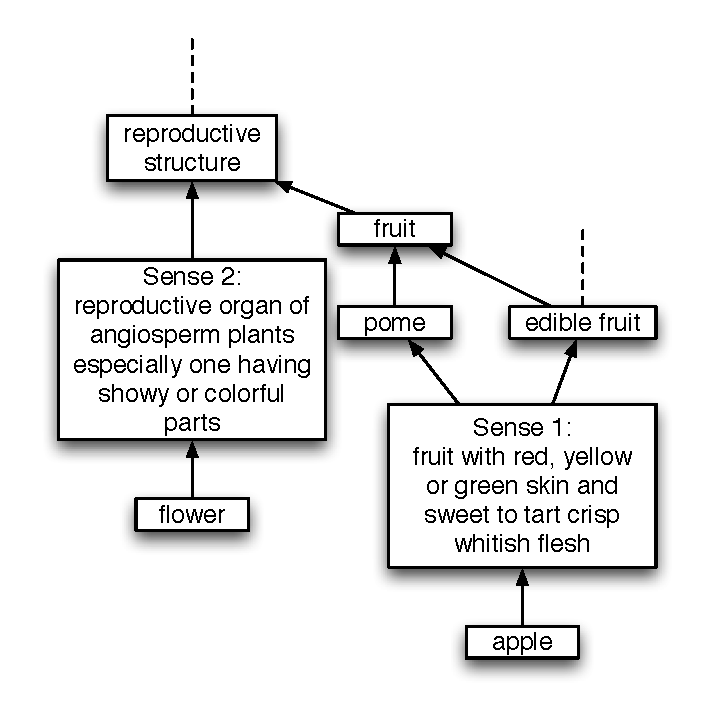
\includegraphics[width=.5\textwidth]{img/flower-apple}
	%}
	%\marginnote{
	%	\begin{minipage}{\marginparwidth}
			\caption{The figure shows respectively matches and mismatches of similarities distributed over sections.}
			\label{fig:sim-analysis}
	%	\end{minipage}
	%}
\end{figure}
The overall average similarities for matching articles is $0.57$ and for mismatching articles it is $0.5$ in a range of $[0;1]$. This seems to be a low match similarity and very high mismatch similarity. The low match similarity could be explained by the definitions of the topics, which might not be the same as what the content providers deem as relevant for these topics. Moreover, the definitions are by no means comprehensive and should more be seen as a subset of their general definitions. The high mismatch similarity average could be explained by the fact that some of the article are actually matches, but are not listed under these topics. An example of this is shown in Figure~\ref{fig:mismatch}.
\begin{figure}[h!tp]
	\myfloatalign
	%\makebox[\textwidth][l]{
		\includegraphics[width=\textwidth]{img/mis-match}
	%}
	\marginnote{
		\begin{minipage}{\marginparwidth}
			\vspace{-120pt}
			\caption{The figure shows an article which has by the system been deemed an article about technology, but is only listed under a business press releases tag by Yahoo.}
			\label{fig:mismatch}
		\end{minipage}
	}
\end{figure}
The fact that most of the used content providers list their feeds under several topics and supplies the articles in all matching feeds could explain this. To handle this, tags were added to the article whenever a URL from the feed was already visited. This did, however, not solve all problems because many content providers listed articles under a different URL for each topic. Looking at the average similarities it is seen that the ``World'' section is near $0.5$ in both matches and mismatches. This could be explained by its definition. It consists mostly proper nouns of parts of the world which are hard to match with proper nouns of countries or cities, that may more often be named in articles.

The similarity between articles is semantically analysed in same way and it is therefore expected to perform equally or better. Better, because the full set of information is available in the article and thereby the analysis has a better chance of extracting keywords, perform enriching and extract entities. It should be noted that the Open Calais API sometimes have problems with extracting entities from a set of keywords instead of sentences, and it could therefore be interesting to explore the possibilities of representing topics based on sentences instead.

In any case, it seems that this analysis is not accurate and a deeper analysis of the similarities in terms of numbers must be done in order to draw any conclusions. However, a qualitative assessment of the results is that the application rarely provides irrelevant articles according to the topics, and that it especially performs well with recognition of entities in articles. And that is even for low similarities. Also, the application seems to be good at following the rules of placing articles that relate near each other, and thereby supplying them in more relevant context than just under the topics, as it is done in conventional newspapers. Finally, some quality of the method can be seen in that the same semantic analysis is done by AdSense and that \cite{116262780379.pdf} has produced promising results with the same algorithm.
%\todo[inline]{Ikke så godt at der ikke har været tid til en ordenlig evaluering... :( Kan ikke lige finde ud af om jeg skal lade være med at skrive det eller hvad.}

It could be interesting to evaluate the precision and recall\sidenote{Precision is the fraction of retrieved instances that are relevant, while recall is the fraction of relevant instances that are retrieved.} points as described in \shortcite{Evaluating-a-User-Model-Based-Personalisation-Architecture-for-Digital-News-Services.pdf}. This could be done by letting a number of test subjects organise a subset of the gathered articles into the given topics and then do an equal analysis as shown in Figure~\ref{fig:mismatch}. Precision and recall evaluation have been done in \cite{Sections-categories-and-keywords-as-interest-specification-tools-for-personalised-news-services.pdf} with categories represented by keywords, it shows poor results for categories of with represented by a few keywords.

In addition, a more comprehensive list of categories and their definitions could also be used. This could either be retrieved by the list of Google News categories\sidenote{\url{http://support.google.com/webmasters/bin/answer.py?hl=en&answer=42993}.} and a WordNet enriched list of key words from Google News list of suggested keywords\sidenote{\url{http://support.google.com/news/publisher/bin/answer.py?hl=en&answer=116037}.} or by the root terms presented in \cite{10-1-1-19-5583}. These can later on be refined by information retrieved by the user behaviour in the system. The user behaviour would also make the system stronger as their relevance feedback can be used to remove false positive and as stated earlier, collaborative filtering to suggest false negatives. The latter could be backed by providing a higher relevance for articles with a subject with many available articles in recent time.
%However, also more advanced techniques of text classification could be used in later stages of the system, like one presented in \shortcite{Evaluating-a-User-Model-Based-Personalisation-Architecture-for-Digital-News-Services.pdf}.
%a Vector Space Model (VSM)
%The paper based on: news items per section, news items per category, maximum number of news items per message required by the user, general relevance of the contents of a given day for a given user, etc. as \cite{Sections-categories-and-keywords-as-interest-specification-tools-for-personalised-news-services.pdf} proposes.
%\cite{Personalizing-your-electronic-newspaper.pdf} suggest virtual communities, or individuals with common interests.

In the application a user could be presented with an article he has seen before. \cite{User-Modeling-for-Adaptive-News-Access.pdf} suggests the nearest neighbour (NN) algorithm approach, using a TF-IDF similarity, to determine whether the story is already known, i.e.\ if the similarity to the NN of articles, that are detected to be already seen, is above a given threshold the article is also determined to be seen. This could be solved by keeping a library of read items and then match new items against this list and down prioritise them if their similarity is too high. However, user might be interested in reading many articles about the same story.
%``Distinguishing between short-term and long-term models has several desirable qualities in domains with temporal characteristics (Chiu and Webb, 1998).'' \cite{User-Modeling-for-Adaptive-News-Access.pdf}.

\cite{Sections-categories-and-keywords-as-interest-specification-tools-for-personalised-news-services.pdf} raise a precision problem in finding relevant news within a single day. This can hopefully be handled by having the user specify in which period of time he wants news and maybe notify the user that solutions might be inaccurate if a limited period of time is chosen, or just provide only articles that are available.
%``just as newspaper must come full of news everyday, regardless of whether anything interesting has happened or not, newspaper sections will carry a certain amount of news independently of their relevance to the section heading, and a personalised news message will feature some news item distantly related to the user profile.''
%Evaluate using the in \shortcite{Evaluating-a-User-Model-Based-Personalisation-Architecture-for-Digital-News-Services.pdf} presented method. Their categorisation based on few keywords (5 as the lowest) to represent a category resulted in poor evaluation, this gives a good motivation for including more keywords and using WordNet to enrich the set of keywords.
%
%\todo[inline]{Maybe find a better example of text classification.}
%
%Use of automatic generation of personal item summaries \cite{fulltext.pdf}

The system does at this point not supply articles of relevance based on the users location. If geo targeting are introduced, using e.g.\ the users IP address or the W3C Geolocation API\sidenote{An effort by the World Wide Web Consortium to standardise an interface to retrieve the geographical location information for a client-side device.}, the system would be able to provide higher relevance according to words that suggest a position on the map. This could also be used to define the ``World'' section even better.
%Use a thesaurus and predefined root terms as in \cite{10-1-1-19-5583} which improves classification; semantic knowledge is more general than keywords.

Furthermore, weights on keywords could be adjusted by a strength (or an uncertainty) of prediction is proposed by \cite{10.1.1.45.5230.pdf}. The uncertainty could be calculated on the basis of how many uses there are of a word, as provided by WordNet.

Finally, some articles presented with the same content over and over again and even contained the main menu of the sites. This was due to some bad results from the scraping using the Readability API. The problem with this is that the menu of news sites often holds keywords that relate to most sections and will therefore be assigned a good relevance to most sections. Because of this, these articles will show up more regularly than others, which disturbs the results from the compositions. Moreover, it could also explain some of the causes to the high relevance mismatch mean derived from the similarity analysis earlier. The problem could be solved with a better sanitising of HTML and standardising of the content. This would remove odd looking elements.

\section{Functionality}
In order to come closer to understanding what conventional newspapers does in terms of editorial rules, it could be interesting to analyse their component structure, e.g.\ using the algorithm presented in \cite{00953970.pdf}. It could also be interesting to establish a co-operation with newspaper editors to extract rules.
%Noget om hvordan programmet samler keywords med vægte for en bruger?
%\todo[inline]{Count the number of sources have included an articles that are very similar to find the breaking factor. Har jeg ikke skrevet det her?}

%$O(n+10 \cdot n(c + c \cdot v + 40n \cdot c \cdot v) )$
The asymptotic running time of the algorithm is $O(m+n^2cv)$, where $m$ is number of articles provided to solve the problem with, $n$ is number of variables in the problem, $c$ is the number of constraints and $v$ is the number of variables a constraint is defined on. This means that the running time is very much dependent on the problem definition, but also of the number of articles given. The function is actually only provided with a subset of the full library based on relevance to spare computation time, but the upper bound remains because it potentially could provide the full library, whereas in practise only a certain percentage constitutes the articles used. More crucially, the running time is polynomially dependent on the number of articles need in the section multiplied by the constraints and the number of variables a constraint is defined on. It is a high running time, but many actions can be taken towards optimising the algorithm, e.g.\ the use of local search techniques, like hill climbing and simulated annealing. Also, the very effective constraint propagation has not been implement, which can aid the algorithm in removing values that are inconsistent with the problem. However, the algorithm is guided to solve the problem both by the MCV heuristic and by the violations of the constraints. Moreover, it is possible to decompose and organise the constraints to aid the algorithm in solving the problem.
%\todo[inline]{hard constraints are not implemented. Should I mention this??}
%Model-View-Control using backbone.js
%Paging: single page web apps + manipulation the browser history \url{https://developer.mozilla.org/en/DOM/Manipulating_the_browser_history}

Furthermore, the CPL only works on finite domains and propagating through many values causes many iterations. Instead it could be interesting to explore a combination of values and ranges in domains. A range could be defined by a start value, a step size and an end value, e.g.\ the list $[0,2,4,6,8,10]$ would be represented by $[0;1]$ with step size $0.2$. This way a whole range could be discarded in a propagation step by looking at its maximum and minimum value. Moreover, if the range holds a potential valid value it can be divided into smaller ranges and their minimum and maximum values may be examined. This divide-and-conquer technique may continue until the search reaches atomic values, which is determined by the step size of the range. If some atomic values and ranges seems to fulfil the constraints they should be kept in the domain.

Moreover, as an answer to the stated hypothesis in section~\vref{sec:hypothesis}, it was possible to personalise the editorial mix and solve the problem with CP and new rules can easily be added or existing ones can be changed. A by-product of the implementation was even a general purpose solver for combinatorial personalisation problems. The library may even be used for other purposes, as long as the problems can be modelled by means of values, variables, domains and constraints. This means that CP was indeed applicable to personalisation problems. The library should, furthermore, be understandable for developers to use it, even if they do not have insight in CP. Finally, it is prepared for implementation of constraint propagation and an automatic ordering of constraints, to optimise the running time for the solver.

% section evaluation (end)
%!TEX root = thesis.tex
\chapter{Discussion} % (fold)
\label{ch:discussion}
%- Evaluate the solution and compare existing techniques for personalisation to the ones used in the solution.
% section discussion (end)

\todo[inline]{Apple vs. apple}
%!TEX root = thesis.tex
\chapter{Conclusion} % (fold)
\label{ch:conclusion}

% section conclusion (end)

%\include{Chapter02} % Chapter 2
%\include{Chapter03} % Chapter 3
%\include{Chapter04} % Chapter 4 - empty template


%----------------------------------------------------------------------------------------
%	THESIS CONTENT - APPENDICES
%----------------------------------------------------------------------------------------

\appendix

\part{Appendix} % New part of the thesis for the appendix

%!TEX root = thesis.tex
\chapter{User Needs}
This section will define the user needs for the application.

\section{Personas}
%http://www.pewinternet.org/Reports/2010/Generations-2010.aspx 2010
%http://epp.eurostat.ec.europa.eu/portal/page/portal/statistics/search_database
%http://epp.eurostat.ec.europa.eu/tgm/table.do?tab=table&init=1&plugin=1&language=en&pcode=tin00097
%Individuals using the Internet for reading / downloading online newspapers / news magazines (tin00097)

\begin{itemize}
	\item \url{student} 35\%, \url{employees self-employed family workers} 31\%, unemployed, retired or other inactive
	\item \url{high formal education} 50\%, medium formal education, no or low formal education
	\item \url{male} 55\%, female
	\item \url{16-24} 34\%, \url{25-54} 34\%, 55-64, 65-74
\end{itemize}

\subsection{Thomas: student medium formal education male 21}
Thomas is 21 and a student at the Technical University of Denmark to be a bachelor of engineering in software. He is very interested in soccer and is therefore always updated on sports news. He reads about it online, newspapers and talks about it with friends. With big events he even likes to post it on Facebook. As a soon-to-be software engineer he has a natural thirst for news about technology, and he mainly reads these at home at the dormitory.
wired.com, newz.dk, engadget.com, facebook.com
computer, Samsung Galaxy Tab

\subsection{Laura: employed high formal education female 39}
Laura is 39 and is employed as a key account manager. She likes to be updated on strategies and economical status of rivalling companies. She is also very interested in politics and likes to discuss this subject with her friends. She reads economical news and likes to be updated on the run.
b.dk, borsen.dk, twitter.com
iPhone, iPad

\subsection{Marie: unemployed no or low formal education female 61}
Marie is 61 and a currently unemployed housekeeper. She spends her day looking for a job and taking care of her pet cat until her husband comes home. She mostly looks for the gossip sections or news about crime or big disasters. She also spends some time reading through the travelling guides as she dreams of going away with her husband.
ekstrabladet.dk, bt.dk, nyhederne.tv2.dk
computer, Lenovo IdeaPad A1

\subsection{Carl: retired or other inactive high formal education male 69}
Carl is a retired professor in psychology. He likes to discuss human behaviour and relation with his acquaintances and is very interested in cultural events. Therefore he often seeks the cultural sections and discussion fora to see what is going on. 
politiken.dk, aok.dk, dr.dk
computer, iPad

\section{Scenarios}
\subsection{Thomas}
Thomas comes home after a day at the study, picks up his tablet computer and opens Editor from the desktop. Editor opens and shows him the front page where all the headlines stories are displayed. The main story is about a new version of the Android OS that has been released today and presses it to read more. The story opens in a full window display with quality images to match the articles. He reads the first section and feels satisfied with the amount of information, but wants to share the information on Facebook, so he clicks share button and writes a comment and posts it on his Facebook wall. He closes the article and returns to the front page. He sees a top story below the main story about Mr. Mærsk Mc-Kinney Møller who has died. It is not a story that falls into his key interests, but as the news is big he is satisfied that he got informed about it. Thomas feels like reading more about technology so he opens the menu and chooses the ``Tech'' section he has installed in the application. The section opens with a head line and a page number to let him know where in his paper he has navigated to and finds an article about a new multicore CPU technology. He has never been interested in CPU technology before, but finds this technology interesting after reading about it, so he opens the application settings and types in keywords about the technology under his ``Tech'' section to keep him updated about it. He also adjusts the ratio between general and personal news, to be less personal as he feels like he needs to broaden his horizon a bit with respect to news. He closes the settings menu and Editor immediately starts updating the articles. Some new articles about CPU technology has been included amongst the articles in the ``Tech'' section after paging through the section and reading some of the most interesting articles he closes the application.

It could be nice if the key words of a story could be or is already highlighted, so he can click it and add it to his positive or negative list.

``Define keywords and user preferences as rules (static and ageing, dynamic)'' \cite{Personalizing-your-electronic-newspaper.pdf}

\subsection{Laura}
Laura is on the train on her way to a business meeting this morning and pulls out her tablet and sees she has one notification from Editor. She opens Editor to get updated on todays news. The front page is displayed and there are headlines from different top articles and a notification is shown in the corner. She presses the notification and the pages turns to show her the article, which opens in full screen. After reading it she wants to see todays headlines, so she presses the back button to return to the paper and presses the return to front page button and the paper turns pages to reach the front page. She scans the page to see if there is any big news about her rivalling companies. There is no breaking news, so she just turns the page to browse the content of todays paper. As she browses the ``Politics'' section of her paper she finds an article about the Prime Minister introducing a new bill about a toll ring around the capitol city. She chooses the article and it is shown in full screen. As she reaches the bottom of the article she sees the comments about it where her friends and most others are against it. She decides to join the discussion and posts a comment on the article wall. She also sees one of her friends has not commented on the article wall and decides to share the article with her as she thinks she would agree with her opinion. She presses the share button and chooses the Editor logo. A list of her friends is shown, some of them who has already read the article is greyed out, but the one she was looking for is not. So she chooses her and a notification is sent to her.

\subsection{Marie}
It is morning and Marie wants to check the news with her coffee in the couch, so she opens Editor from her tablet to get updated. The front page is displayed with a collection of stories as highlights of the content of the paper. It mainly contains stories about celebrities and a big disaster that has happened in japan, but there is also a story about a big political change, that she does not find interesting. So she goes to the settings menu and types in ``politics'' to add to her negative list. She also adjusts the personal/general news ratio to contain only personal news as she wants only news that is directed to her. She returns to the front page which is now free of political stories. Her newspaper contains many images and videos as she has set her graphical/textual content ratio more towards graphical content.

\subsection{Carl}
Cultural, funnies

\section{Business Case}

\subsection{Need}
User value: personal quality fresh stories (content providers should be chosen!) enriched with quality images. Same navigation as actual newspapers, but faster. Instantly up-to-date. Adaptive layout. Adjustable user profile.

\subsection{Approach}
personalised content + layout.

Constraint Programming: fast computation - good for optimal solutions, describes the generic solution in stead of how to solve or find it, very easy to tailor the problem definition of the solution and adjust it and even let users make the adjustments, transparent.

Content providers can get to know their readers preferences better and improve the provided content.

\subsection{Benefit Per Cost}
revenue flow: Content providers are paid. Income from advertisers (scattered \cite[p. 6-7]{kristin_fredrik.pdf}) and users. Income from selling user behaviour. Free version w. commercials + paid (monthly) without.

\subsection{Competition}
Flip board, Wired magazine and app with actual editors affiliated.

\todonote{Which design choices to focus on?}

\begin{itemize}
	\item ``open, turn pages, chose article, read and return'' \cite[p. 6]{FULLTEXT01.pdf}
	\item both general and personal news (collaborate filtering solves that some news are not received, but are universally interesting \cite{fulltext.pdf})
	\item full screen display of article
	\item images + video? adjustable
	\item graphical/textual content ratio
	\item opens in front page view (summery of newspaper 8 articles) \cite[p. 8]{kristin_fredrik.pdf}
	\item put in personalised sections
	\item back page, funnies?
	\item section headline \cite[p. 6-7]{kristin_fredrik.pdf}
	\item article headlines
	\item article summaries / extracts \cite{fulltext.pdf}
	\item menu w. section headlines \cite[p. 8]{kristin_fredrik.pdf}
	\item page numbers \cite[p. 6-7]{kristin_fredrik.pdf}
	\item page turn
	\item press ``like'' or key word based user profile (mark self or highlighted? right click to add): positive + negative list (keywords+categories \cite{10-1-1-19-5583}, \cite{fulltext.pdf} and \cite{gervasum2001ws.pdf})
	\item adjust variables
	\item share social network
	\item share directly (grey out the ones who have read it)
	\item comment
	\item see friends comments
\end{itemize}

\section{Technical Requirements}
\begin{itemize}
	\item ``the clear overview of content, including a beginning and an end, the ease of use, typography and design'' \cite[p. 7]{FULLTEXT01.pdf}
	\item familiarity in design from printed paper \cite[p. 7]{FULLTEXT01.pdf}
	\item  ``news valuation, e.g. positioning of lead story'' \cite[p. 7]{FULLTEXT01.pdf}
	\item  mobility \cite[p. 7]{FULLTEXT01.pdf}
	\item  continuous updates \cite[p. 7]{FULLTEXT01.pdf}
	\item  ability to search \cite[p. 7]{FULLTEXT01.pdf}
	\item  ``easy and intuitive navigation'' \cite[p. 7]{FULLTEXT01.pdf}
	\item add video and sound \cite[p. 7]{FULLTEXT01.pdf}
	\item Landscape + portrait \cite[p. 6-7]{kristin_fredrik.pdf}
	\item touch screen interaction \cite[p. 6-7]{kristin_fredrik.pdf}
	\item Design+layout from printed newspaper \cite{hcii2005_1004.pdf}
	\item Functionality from online newspaper \cite{hcii2005_1004.pdf}
	\item Name of columnist \cite[p. 4]{gervasum2001ws.pdf}
	\item Transparency of implicit relevance feedback (see/modify current weights of categories) \cite[p. 7]{gervasum2001ws.pdf}
	\item dynamic short-term + static long-term user profile \cite{10-1-1-19-5583}, \cite{fulltext.pdf} and \cite{gervasum2001ws.pdf}
	\item relevance feedback \cite{10-1-1-19-5583}, \cite{fulltext.pdf} and \cite{gervasum2001ws.pdf}
\end{itemize}

In which period of time is an article relevant to a user? Maybe if it is still available, then it is still interesting - new approaches or discussion about the subject might arise. How do we control that a news item is not missed? Keep index of what has been viewed in addition to what has been read. % Appendix A
%!TEX root = thesis.tex
\chapter{Newspaper Topics}
\label{appendix:newspaper-topics}

\begin{table}[h!tp]
\myfloatalign
	%\marginnote{
		%\begin{minipage}{\marginparwidth}
		%\vspace{-100pt}
		\caption{Topic specification}
		\label{tab:topic-specification1}
		%\end{minipage}
	%}
	\makebox[\textwidth][l]{
	\begin{tabular}{p{.15\largefigure}|p{.15\largefigure}|p{.45\largefigure}}
		\toprule
			\textbf{Name}& \textbf{Tags}& \textbf{Keywords (weights)}\\ 
		\midrule
			Technology& technology, science& technology (1.0), mobile (0.6), social\_media (0.8), context-aware (0.3), Javascript (0.6), HTML\_5 (1.0), CSS\_3 (1.0), Web (0.9), Android (0.4), Mac\_OSX (0.5), Windows (0.2), iPhone (0.5), Apple\_Inc. (0.7), Google (0.5)\\
		\midrule
			Science &science &science (1.0),software (0.6), software\_technology (0.8), engineer (0.4)\\
		\midrule
			Sport &sport &Sports (1.0), NFL (0.5), football (0.9), soccer (0.9), NBA (0.5), NCAA (0.5), NHL (0.5), baseball (0.5), golf (0.5), tennis (0.5)\\
		\midrule
			Entertainment &entertainment &entertainment (1.0), art (0.5), celebrity (0.2), fashion (0.3), TV (0.2), Television (0.2), television\_show (0.4), play (0.3), opera (0.2), cinema (0.7), theatre (0.3), read (0.7), hobby (0.5), fun (0.6), enjoy (0.5), laughter (0.5), social (0.2), cartoon (0.4), review (0.7), movie (0.7), book (0.5), music (0.9), picture (0.6)\\
		\bottomrule
	\end{tabular}
	}
\end{table}

\begin{table}[h!tp]
\myfloatalign
	%\marginnote{
		%\begin{minipage}{\marginparwidth}
		%\vspace{-100pt}
		\caption{Topic specification  (continued)}
		\label{tab:topic-specification2}
		%\end{minipage}
	%}
	\makebox[\textwidth][r]{
	\begin{tabular}{p{.15\largefigure}|p{.15\largefigure}|p{.45\largefigure}}
		\toprule
			\textbf{Name}& \textbf{Tags}& \textbf{Keywords (weights)}\\
		\midrule
			Politics &politics &politics (1.0), democrat (0.7), liberal (0.7), government (0.5), state (0.5), corporate (0.4), policy (1.0), authority (0.4), power (0.3), democracy (0.7)\\ 
		\midrule
			Business &business, money &business (1.0), money (1.0), organization (0.7), trade (0.9), goods (0.5), service (0.4), stock (0.4), market (0.8), consumer (0.6), economy (1.0), profit (0.8), owner (0.4), administer (0.4), CEO (0.6), company (0.8), work (0.5), commercial (0.4), proprietorship (0.7), partnership (0.7), corporation (0.7), cooperative (0.4), debt (0.4), value (0.4), payment (0.5), bank (0.6), currency (0.5), account (0.3), savings (0.3)\\
		\midrule
			World &world &world (1.0), international (1.0), Europe (0.6), Middle\_East (0.6), Australia (0.6), New\_Zealand (0.6), USA (0.4), Africa (0.6), Latin\_America (0.6), Asia (0.6)\\
		\midrule
			Health &health &health (1.0), wellness (1.0), fitness (1.0), diet (0.6), weight\_loss (0.5), well-being (0.6), nutrition (0.7), parenting (0.5), health\_care (0.6), pregnancy (0.5), cancer (0.3), allergies (0.6), asthma (0.6), family (0.7)\\
		\bottomrule
	\end{tabular}
	}
\end{table}
%\include{Chapter0B} % Appendix B - empty template

%----------------------------------------------------------------------------------------
%	POST-CONTENT THESIS PAGES
%----------------------------------------------------------------------------------------


\cleardoublepage\include{FrontBackmatter/Bibliography} % Bibliography

%\cleardoublepage\include{FrontBackmatter/Colophon} % Colophon

%\cleardoublepage\include{FrontBackmatter/Declaration} % Declaration

%----------------------------------------------------------------------------------------

\end{document}